\section{测试}
\subsection{业务逻辑层服务}
业务逻辑层服务众多,如第四章介绍的,但测试流程基本上相同,这里只拿典型举例:
\subsubsection{获取车站布局测试}
测试输入(其中的实例id是之前创建的):
\begin{lstlisting}
query {
  stationLayout(id: "db42f0ed-d096-4805-b048-909e69dd44e2") {
    title,
    nodes{
      nodeId, 
      trackId, 
      leftP{x,y}, 
      rightP{x,y}, 
      leftJoint, 
      rightJoint
    },
    signals{
      signalId,
      sgnType,
      sgnMnt,
      protectNodeId,
      side,
      dir,
      pos{x,y},
      btns
    }
  }
}
\end{lstlisting}

服务输出:
\begin{lstlisting}
{
  "data": {
    "stationLayout": {
      "nodes": [
        {
          "leftJoint": "EMPTY",
          "leftP": {
            "x": 0,
            "y": 5
          },
          "nodeId": 1,
          "rightJoint": "NORMAL",
          "rightP": {
            "x": 5,
            "y": 5
          },
          "trackId": "X3JG"
        },
        {
          "leftJoint": "NORMAL",
          "leftP": {
            "x": 5,
            "y": 5
          },
          "nodeId": 5,
          "rightJoint": "NORMAL",
          "rightP": {
            "x": 5,
            "y": 10
          },
          "trackId": "IAG"
        }
      ],
      "signals": [
        {
          "btns": [
            "PASS",
            "GUIDE",
            "TRAIN"
          ],
          "dir": "LEFT",
          "pos": {
            "x": 5,
            "y": 5
          },
          "protectNodeId": 5,
          "sgnMnt": "POST_MOUNTING",
          "sgnType": "HOME_SIGNAL",
          "side": "UPPER",
          "signalId": "X"
        }
      ],
      "title": "测试站"
    }
  }
}
\end{lstlisting}
\subsection{控制台界面}
\begin{figure}[htbp!]
    \centering
    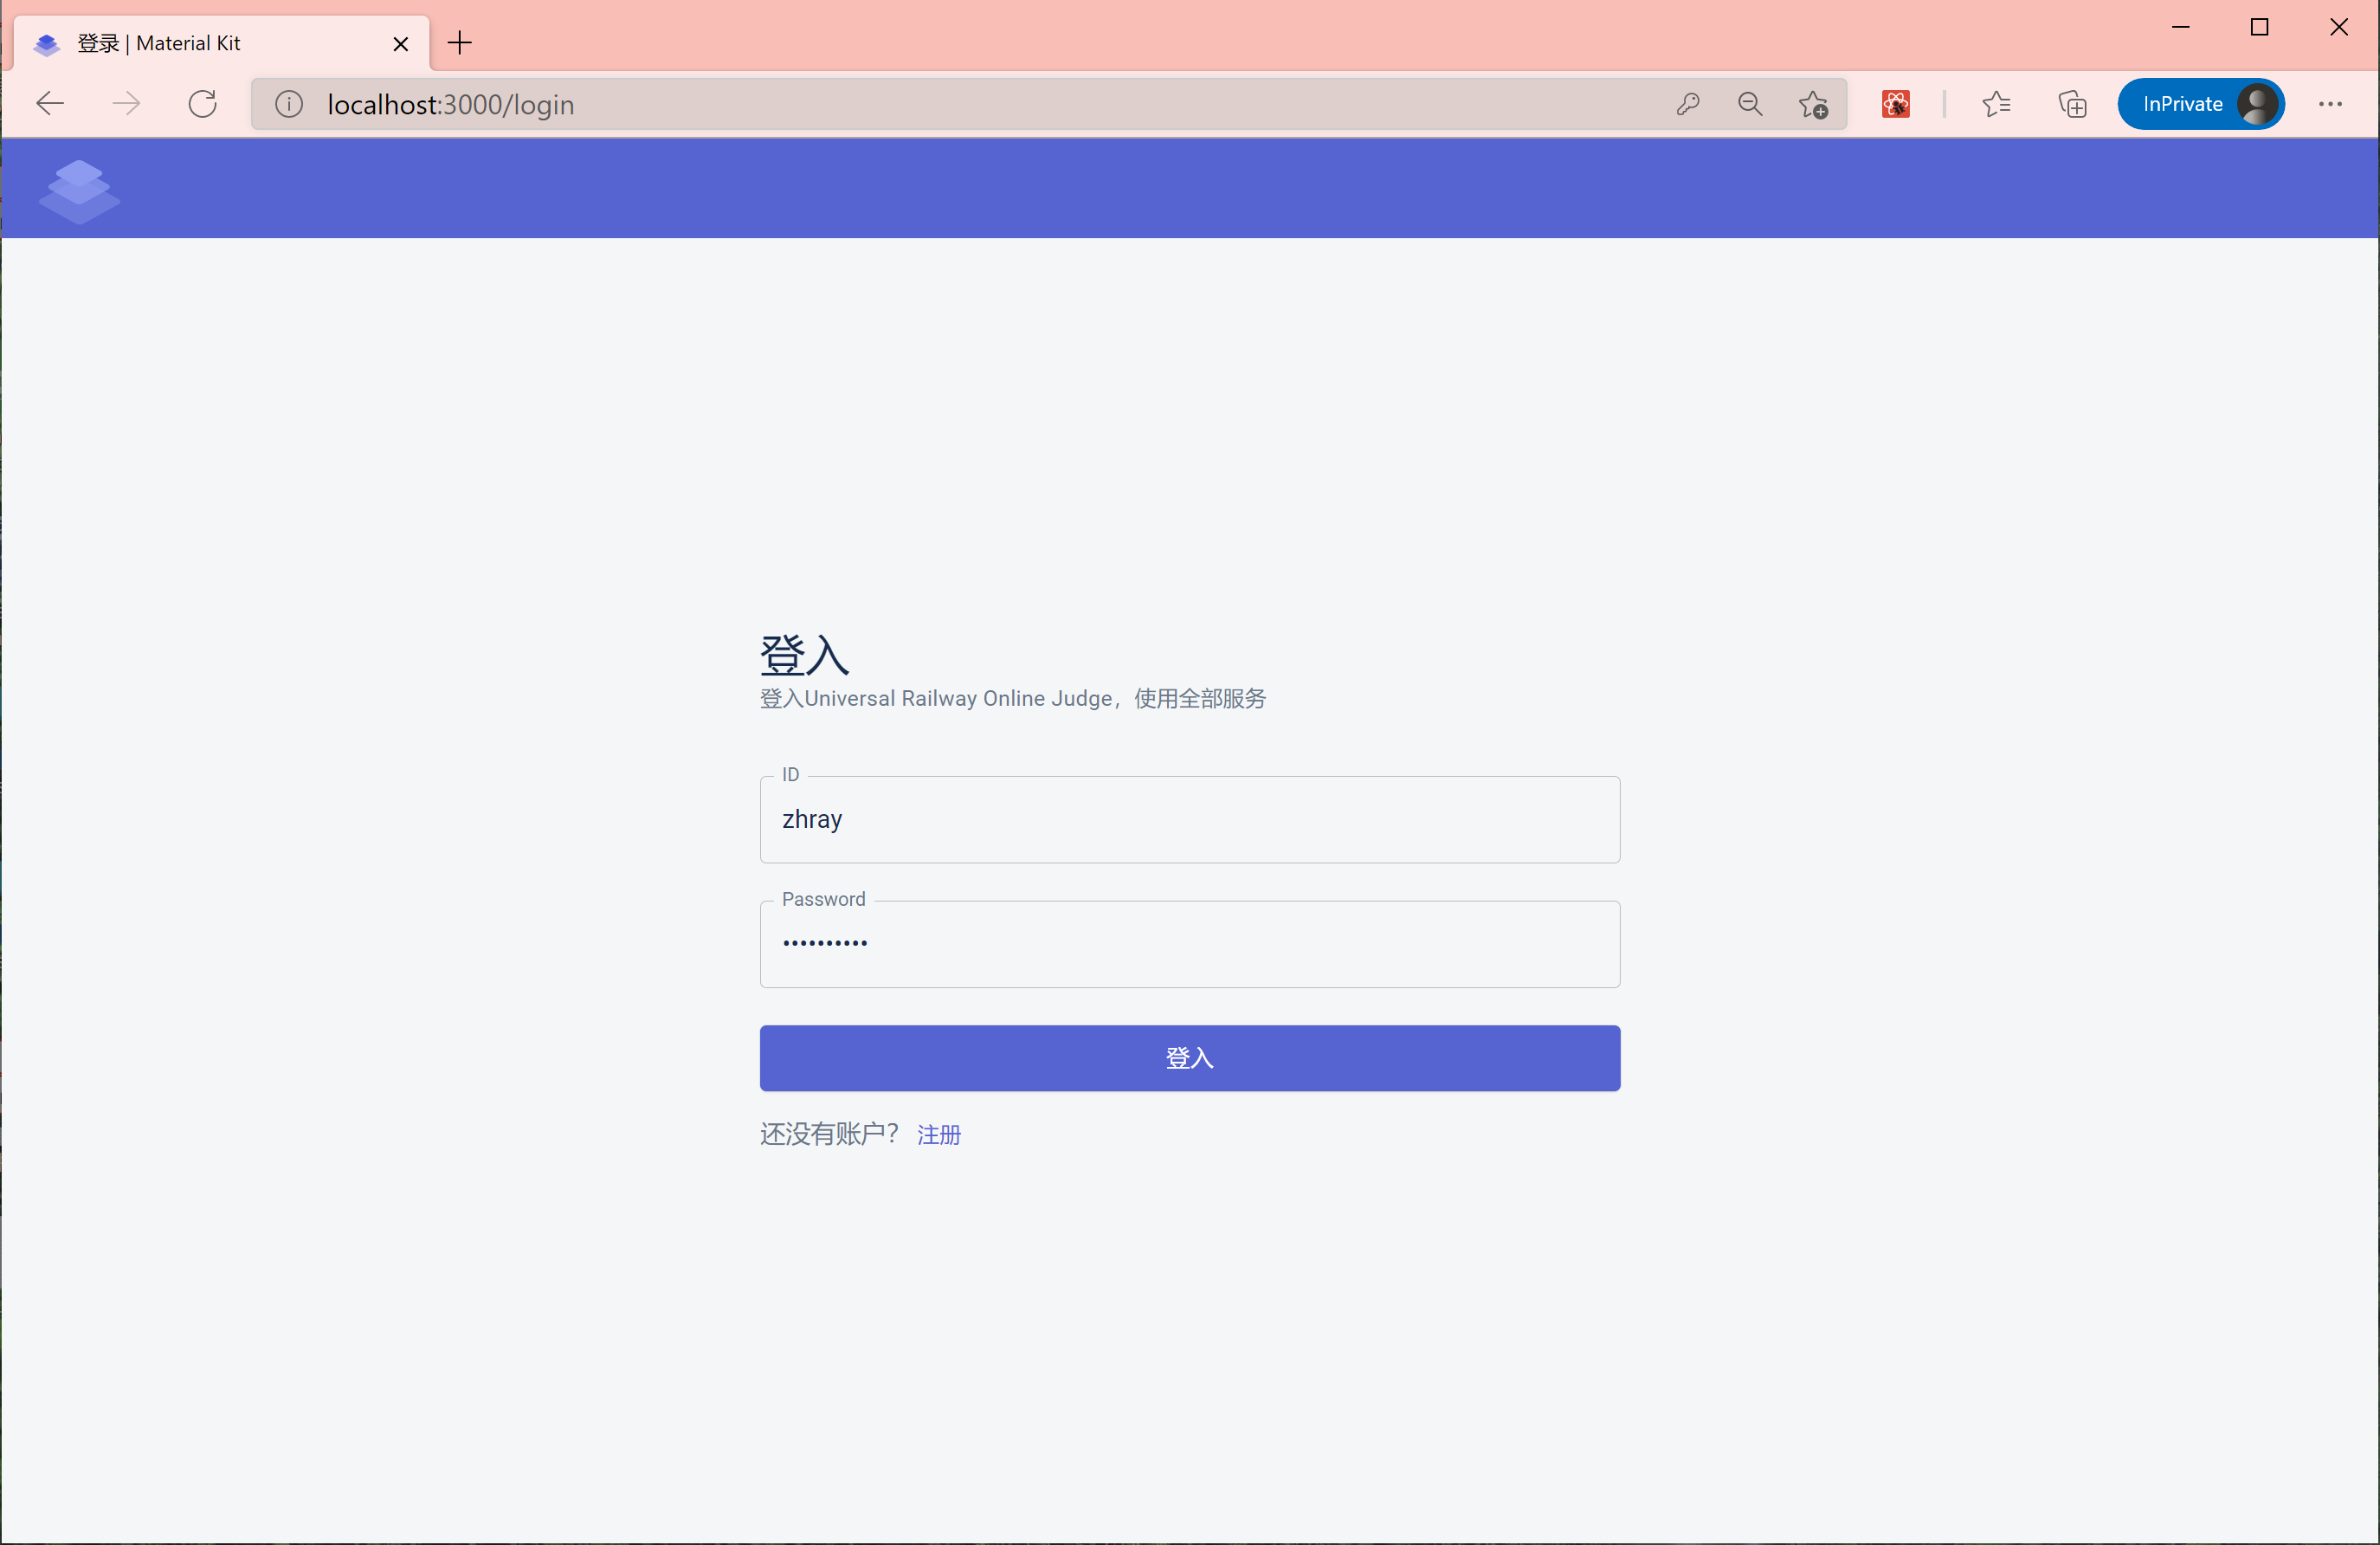
\includegraphics[width=\textwidth]{figures/png/login.png}
    \caption{\label{login}登录界面}
\end{figure}

\begin{figure}[htbp!]
    \centering
    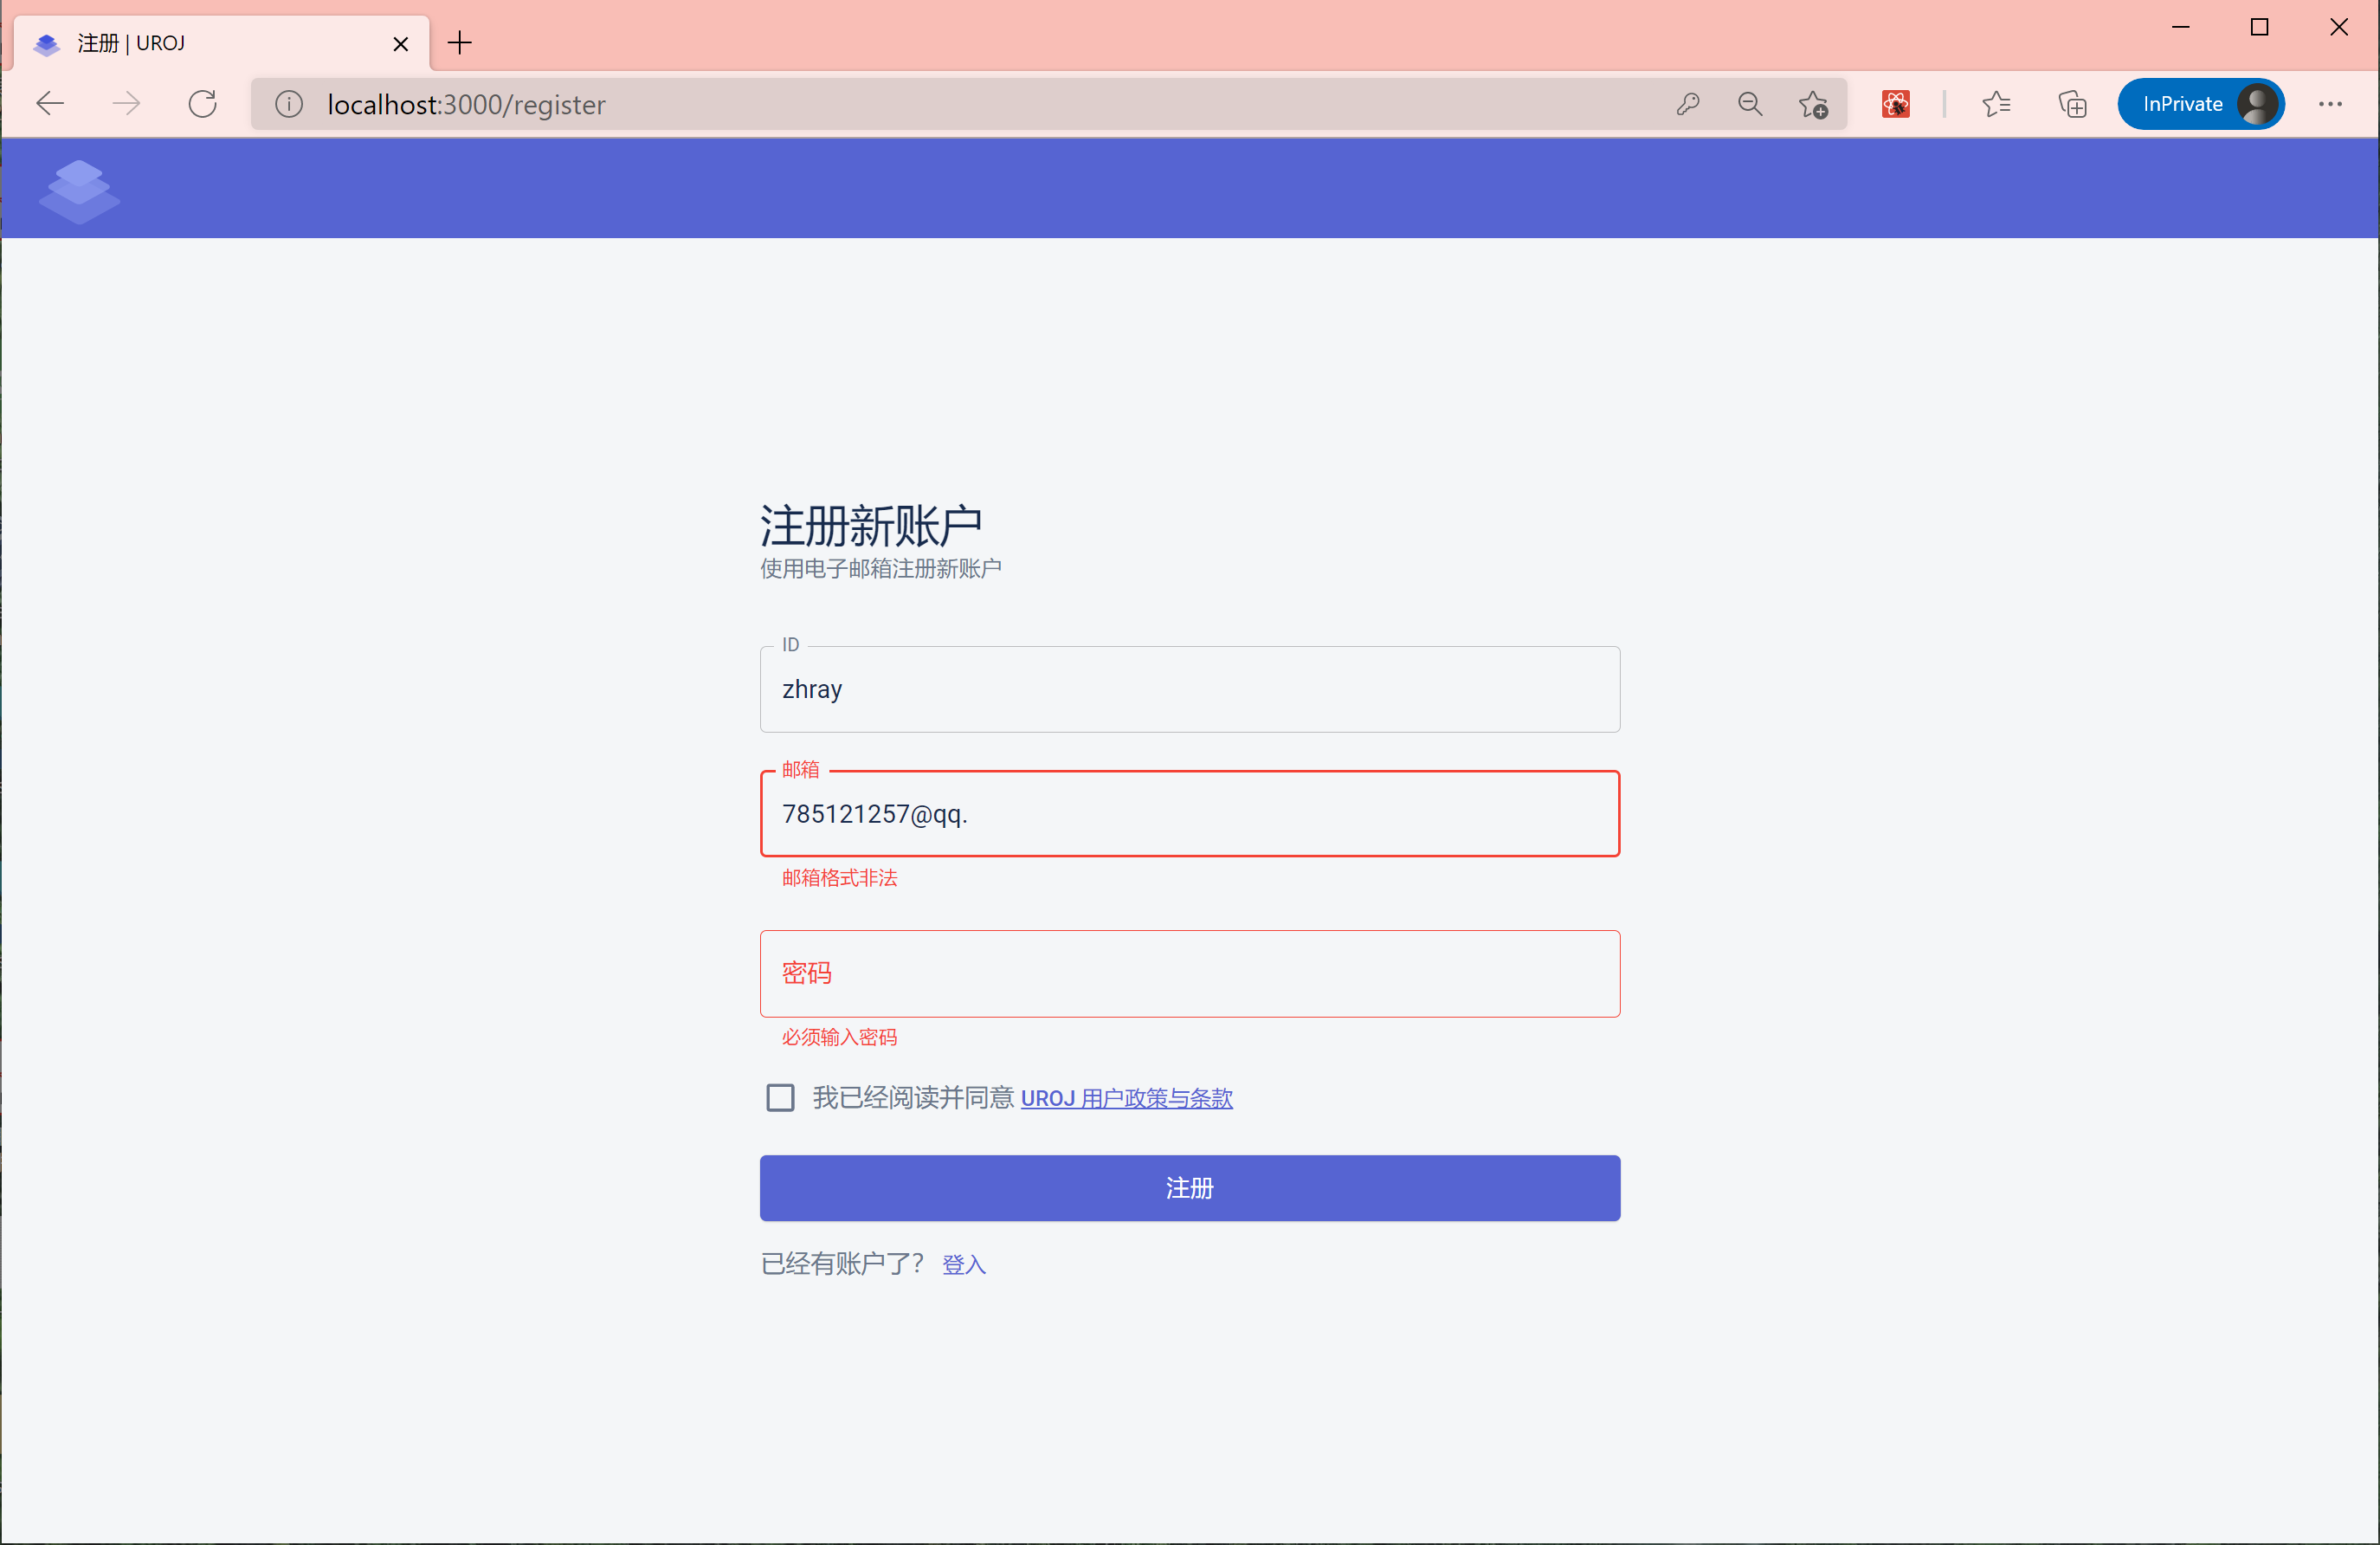
\includegraphics[width=\textwidth]{figures/png/input_err.png}
    \caption{\label{input_err}注册}
\end{figure}

\begin{figure}[htbp!]
    \centering
    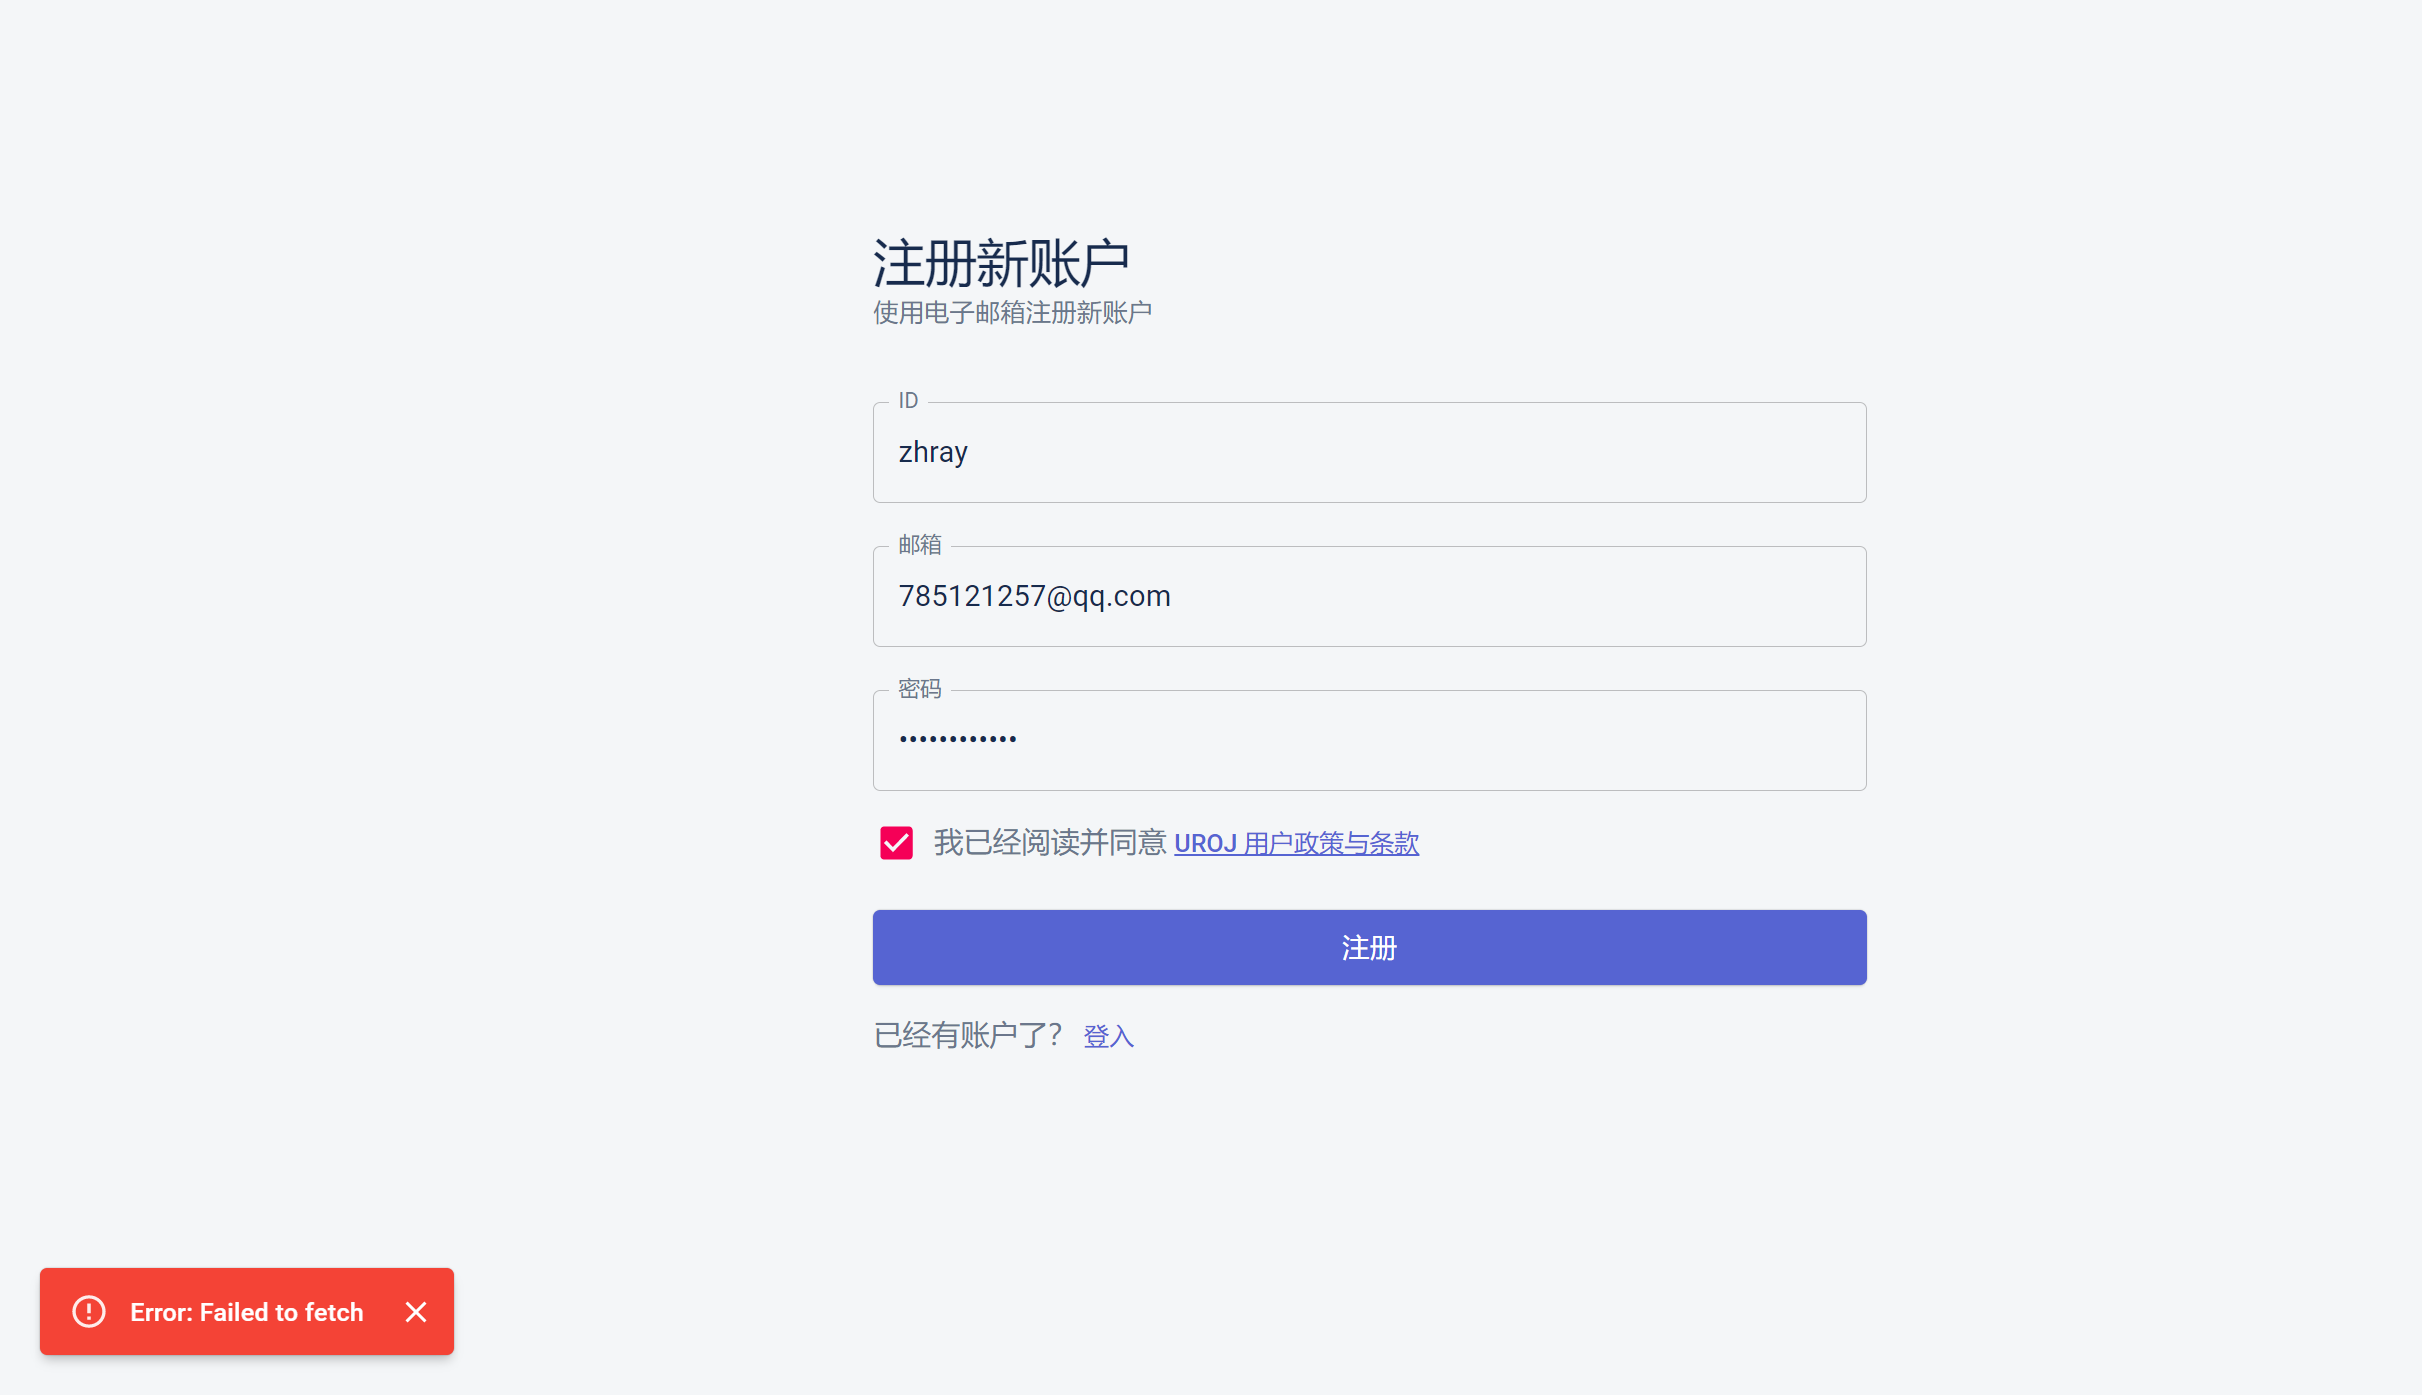
\includegraphics[width=\textwidth]{figures/png/alert_err.png}
    \caption{\label{alert_err}注册失败}
\end{figure}

\begin{figure}[htbp!]
    \centering
    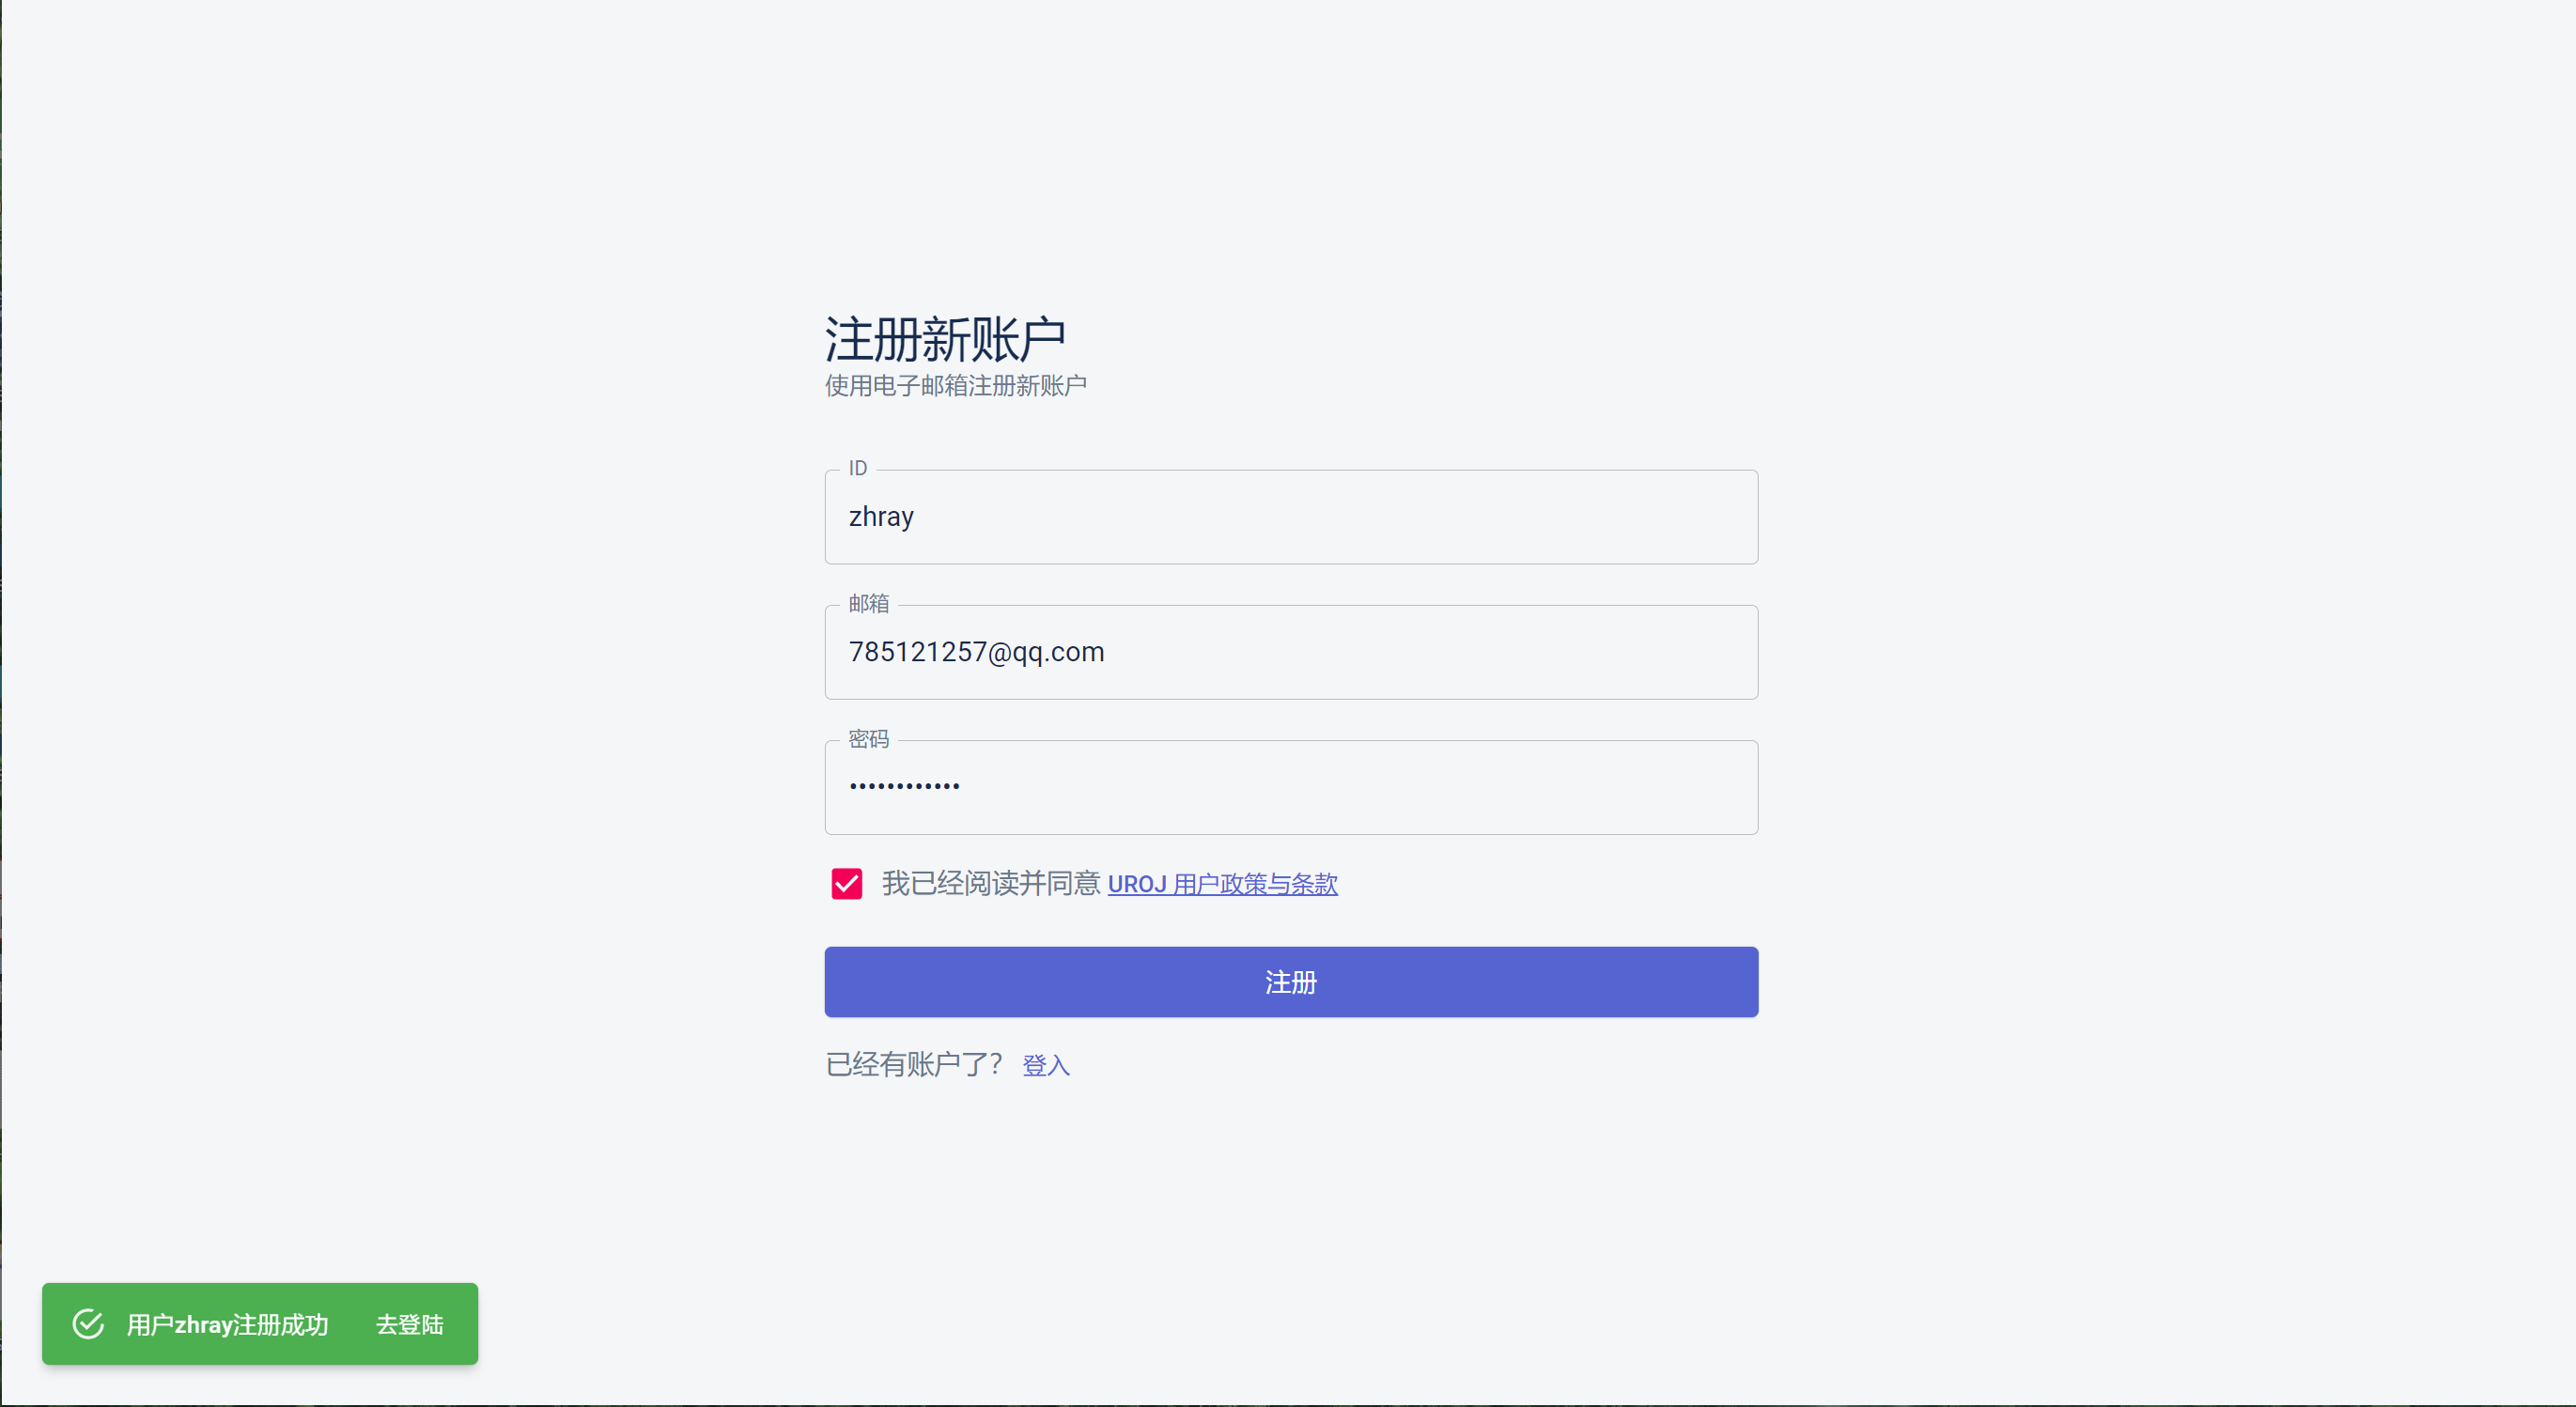
\includegraphics[width=\textwidth]{figures/png/reg_succ.png}
    \caption{\label{reg_succ}注册成功}
\end{figure}

\begin{figure}[htbp!]
    \centering
    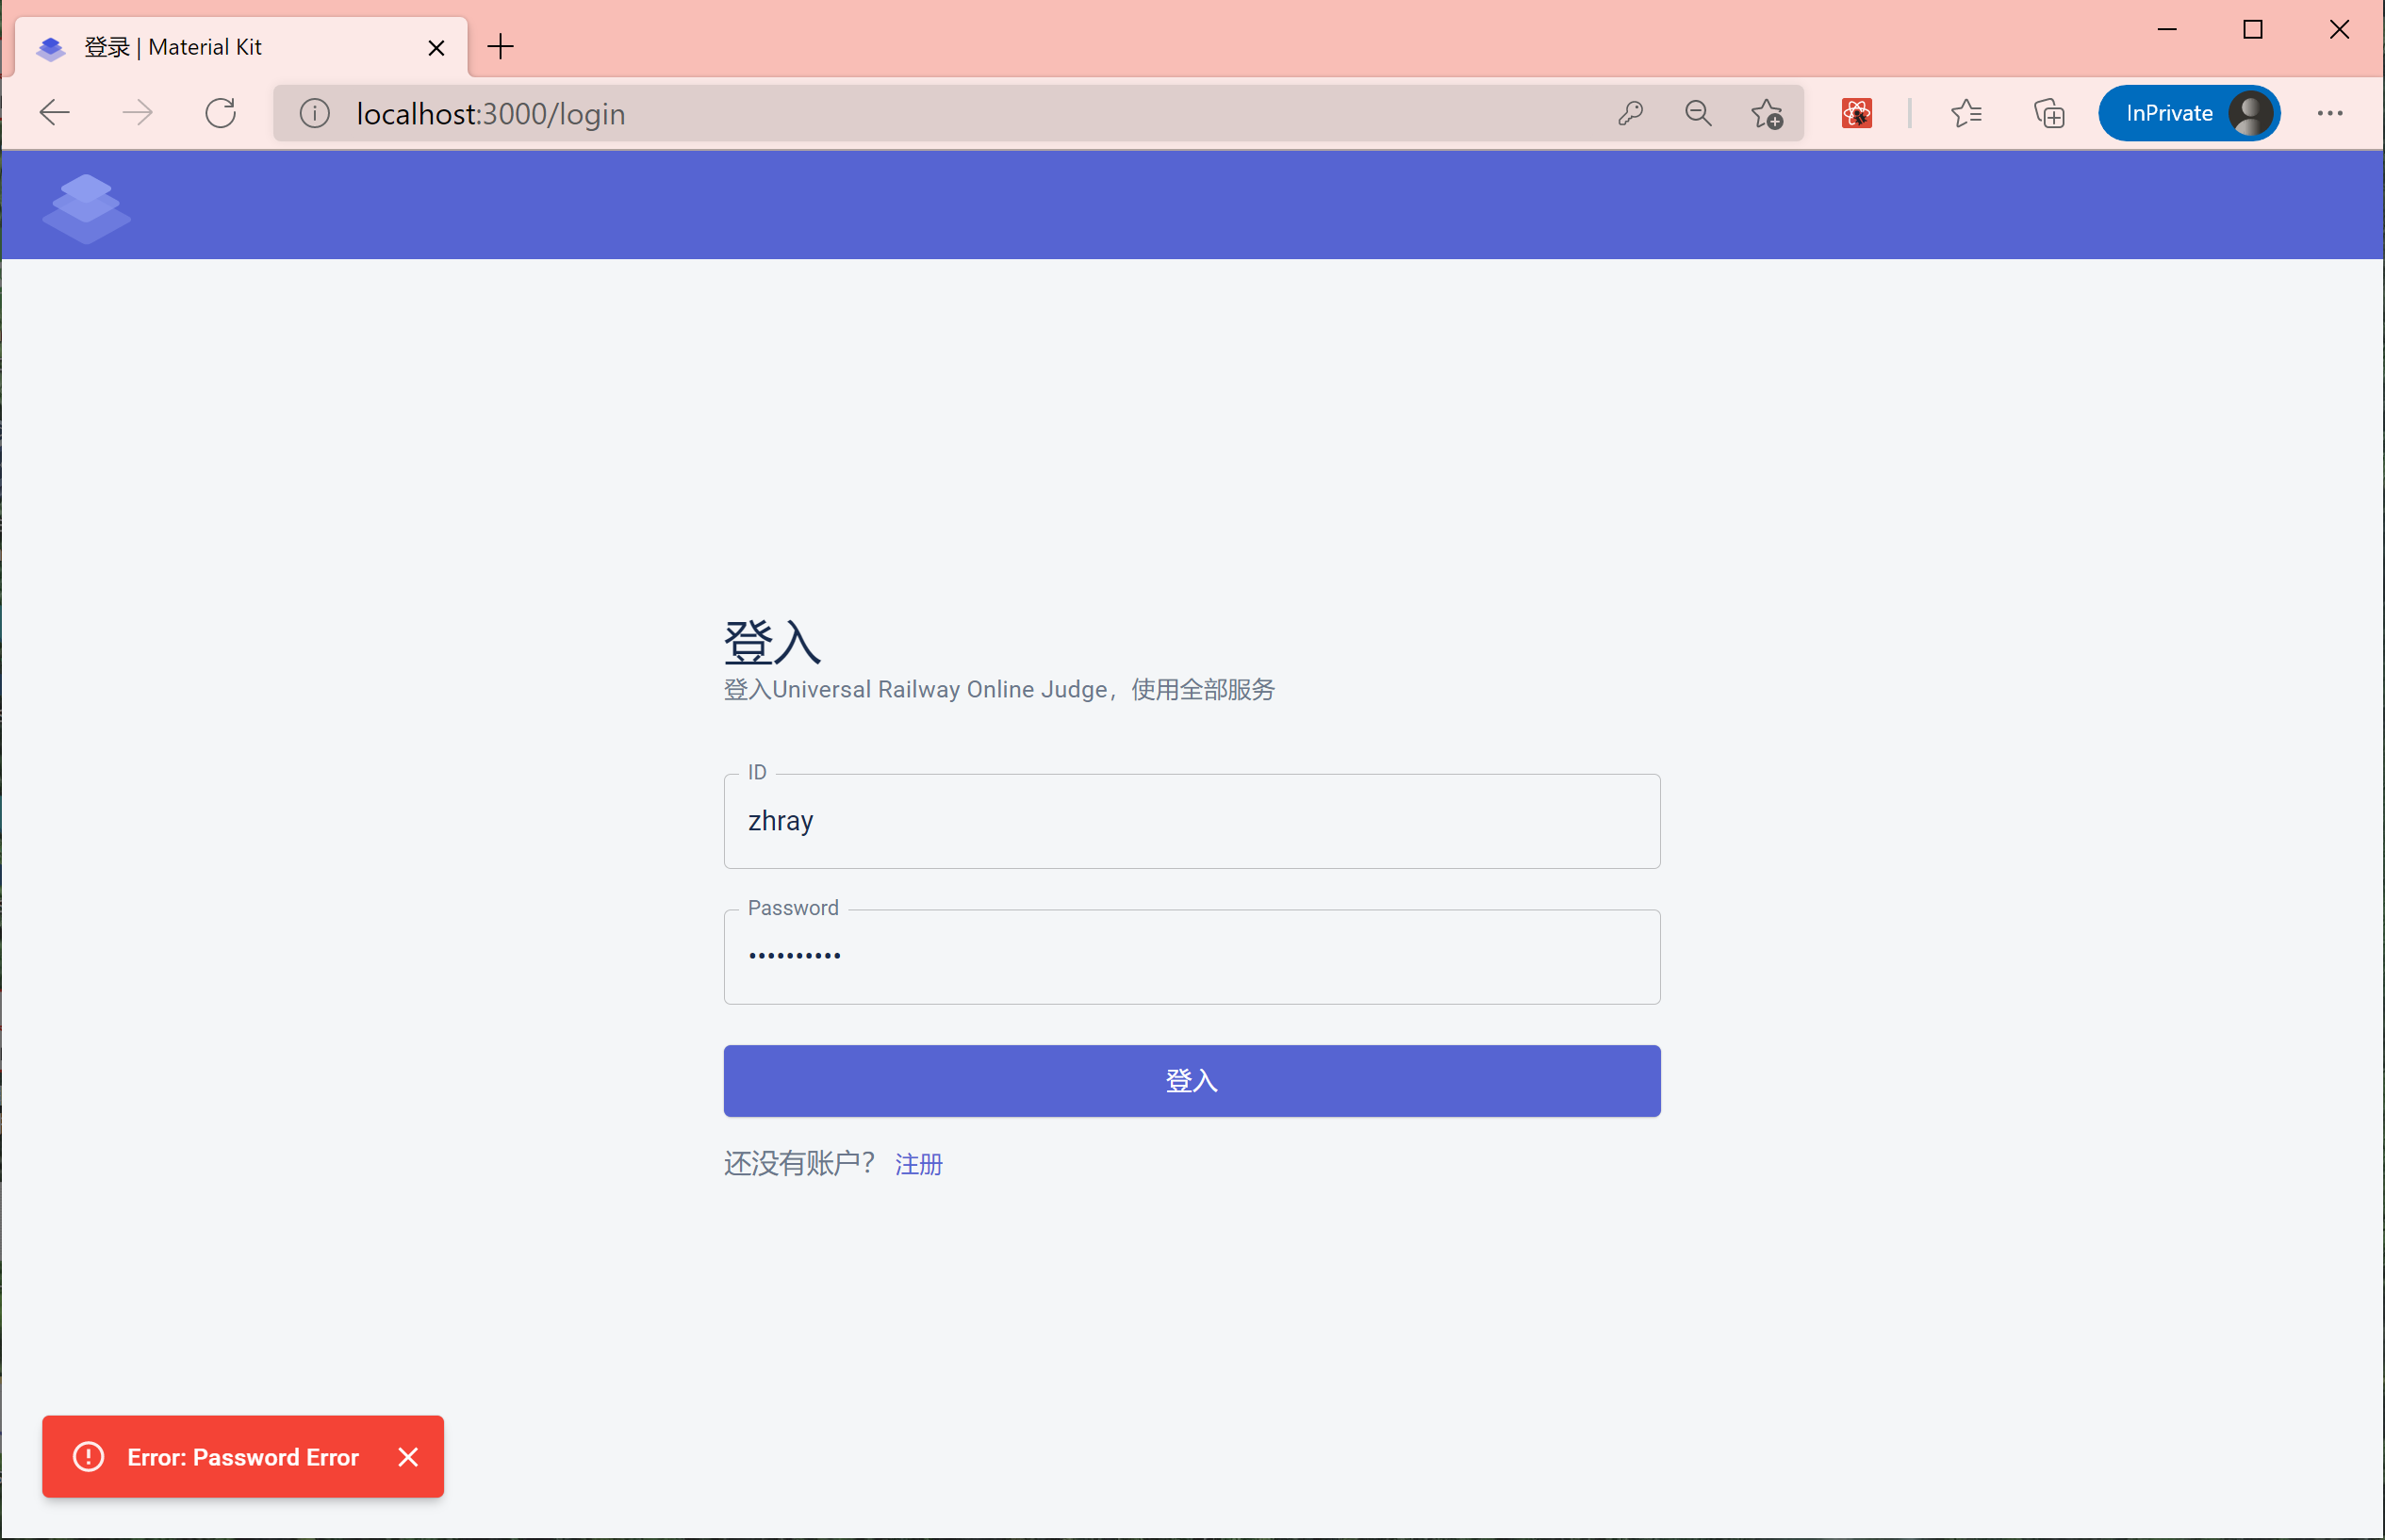
\includegraphics[width=\textwidth]{figures/png/pwd_err.png}
    \caption{\label{pwd_err}密码错误}
\end{figure}

\begin{figure}[htbp!]
    \centering
    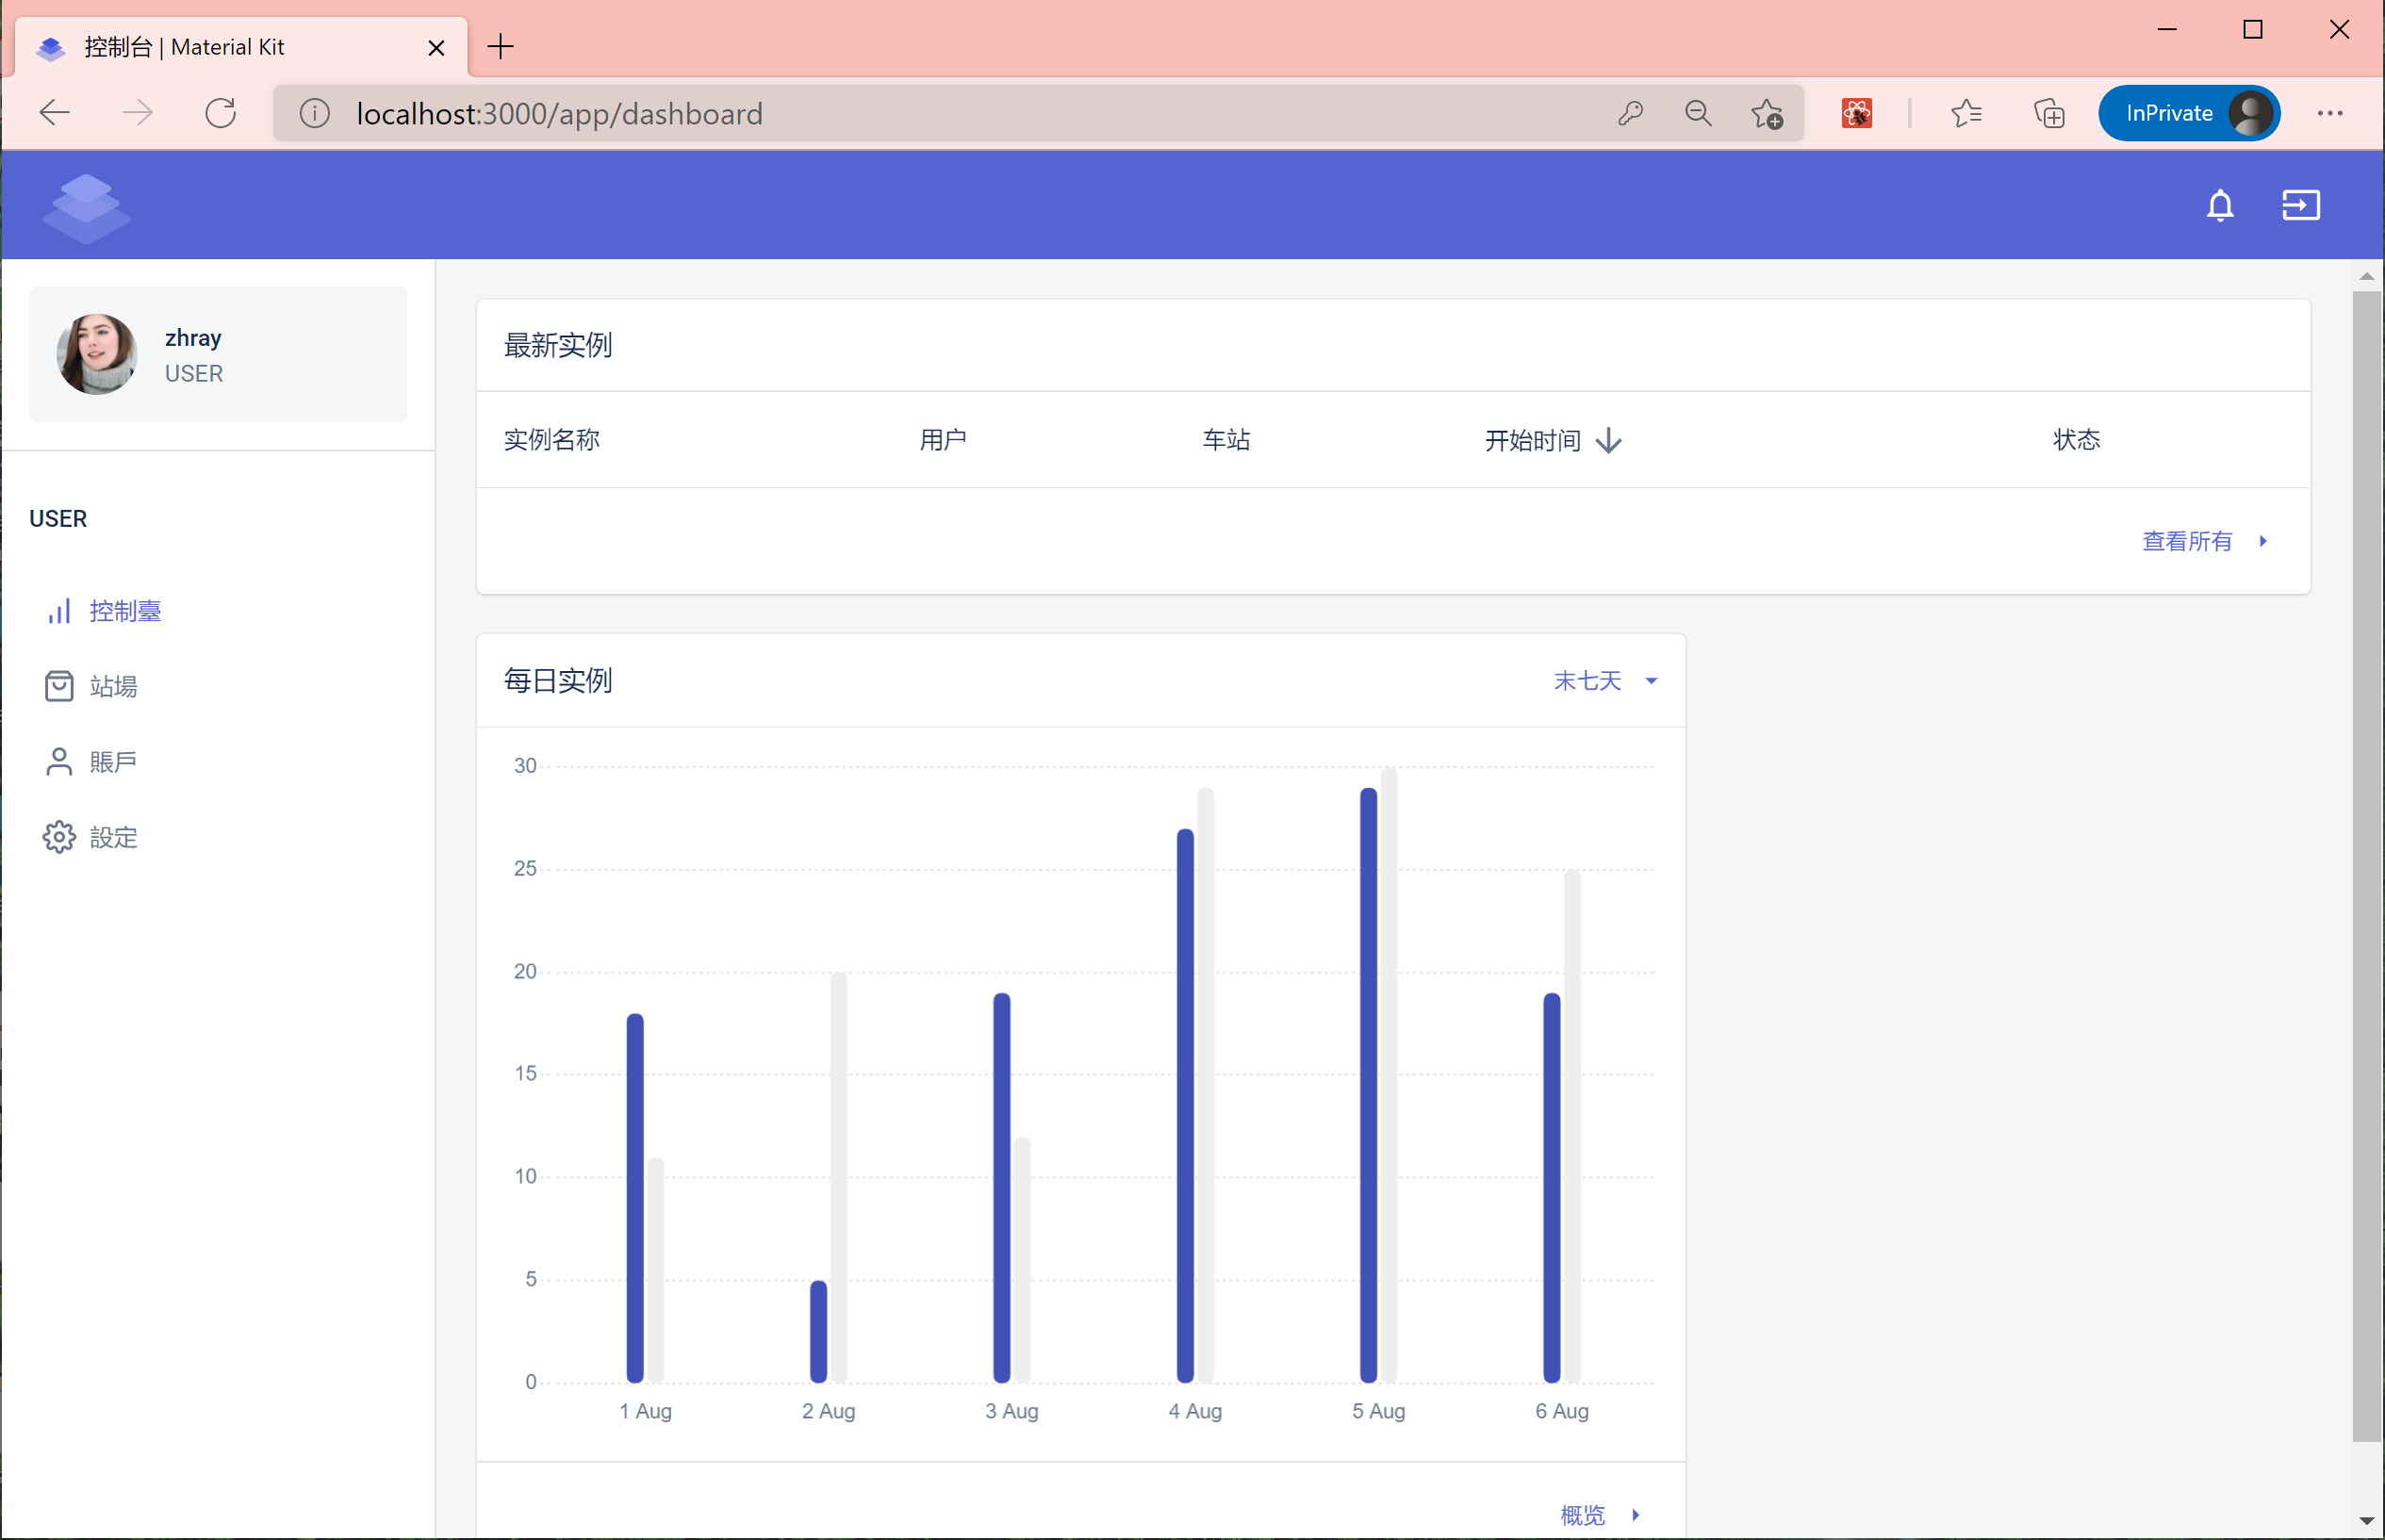
\includegraphics[width=\textwidth]{figures/png/user_ui.png}
    \caption{\label{user_ui}用户角色的控制台首页}
\end{figure}

\begin{figure}[htbp!]
    \centering
    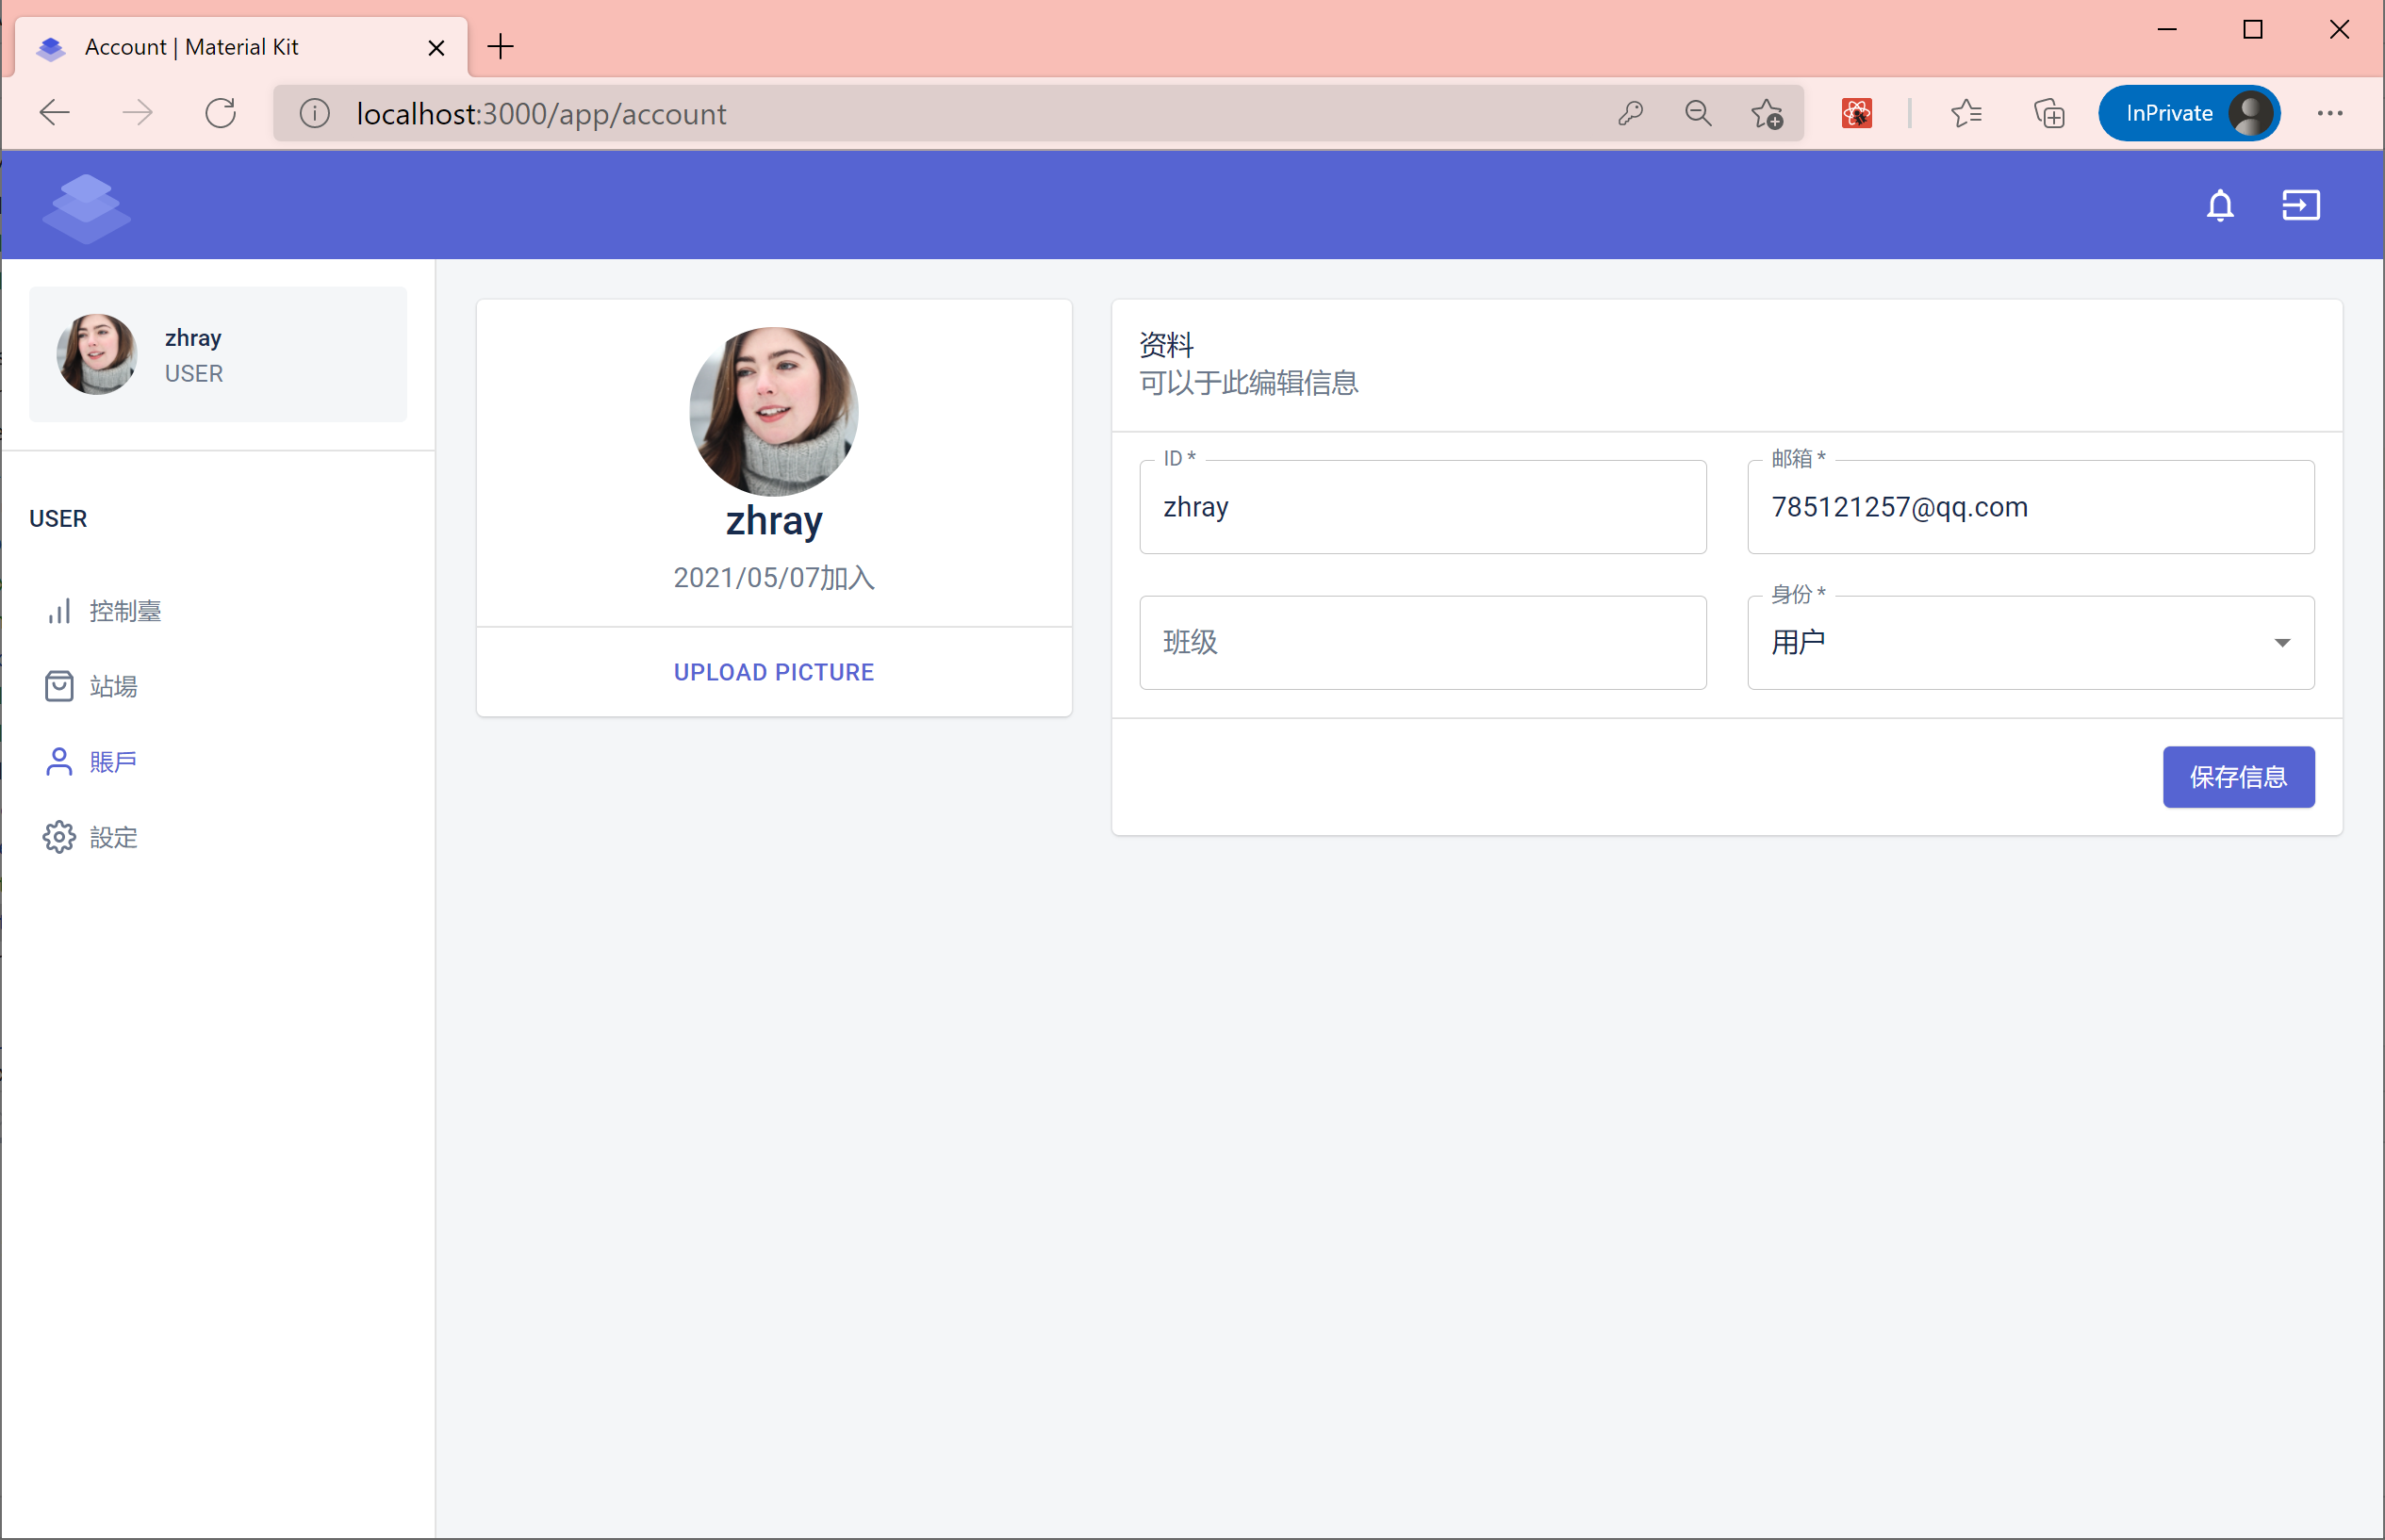
\includegraphics[width=\textwidth]{figures/png/user_data.png}
    \caption{\label{user_data}用户信息页}
\end{figure}

\begin{figure}[htbp!]
    \centering
    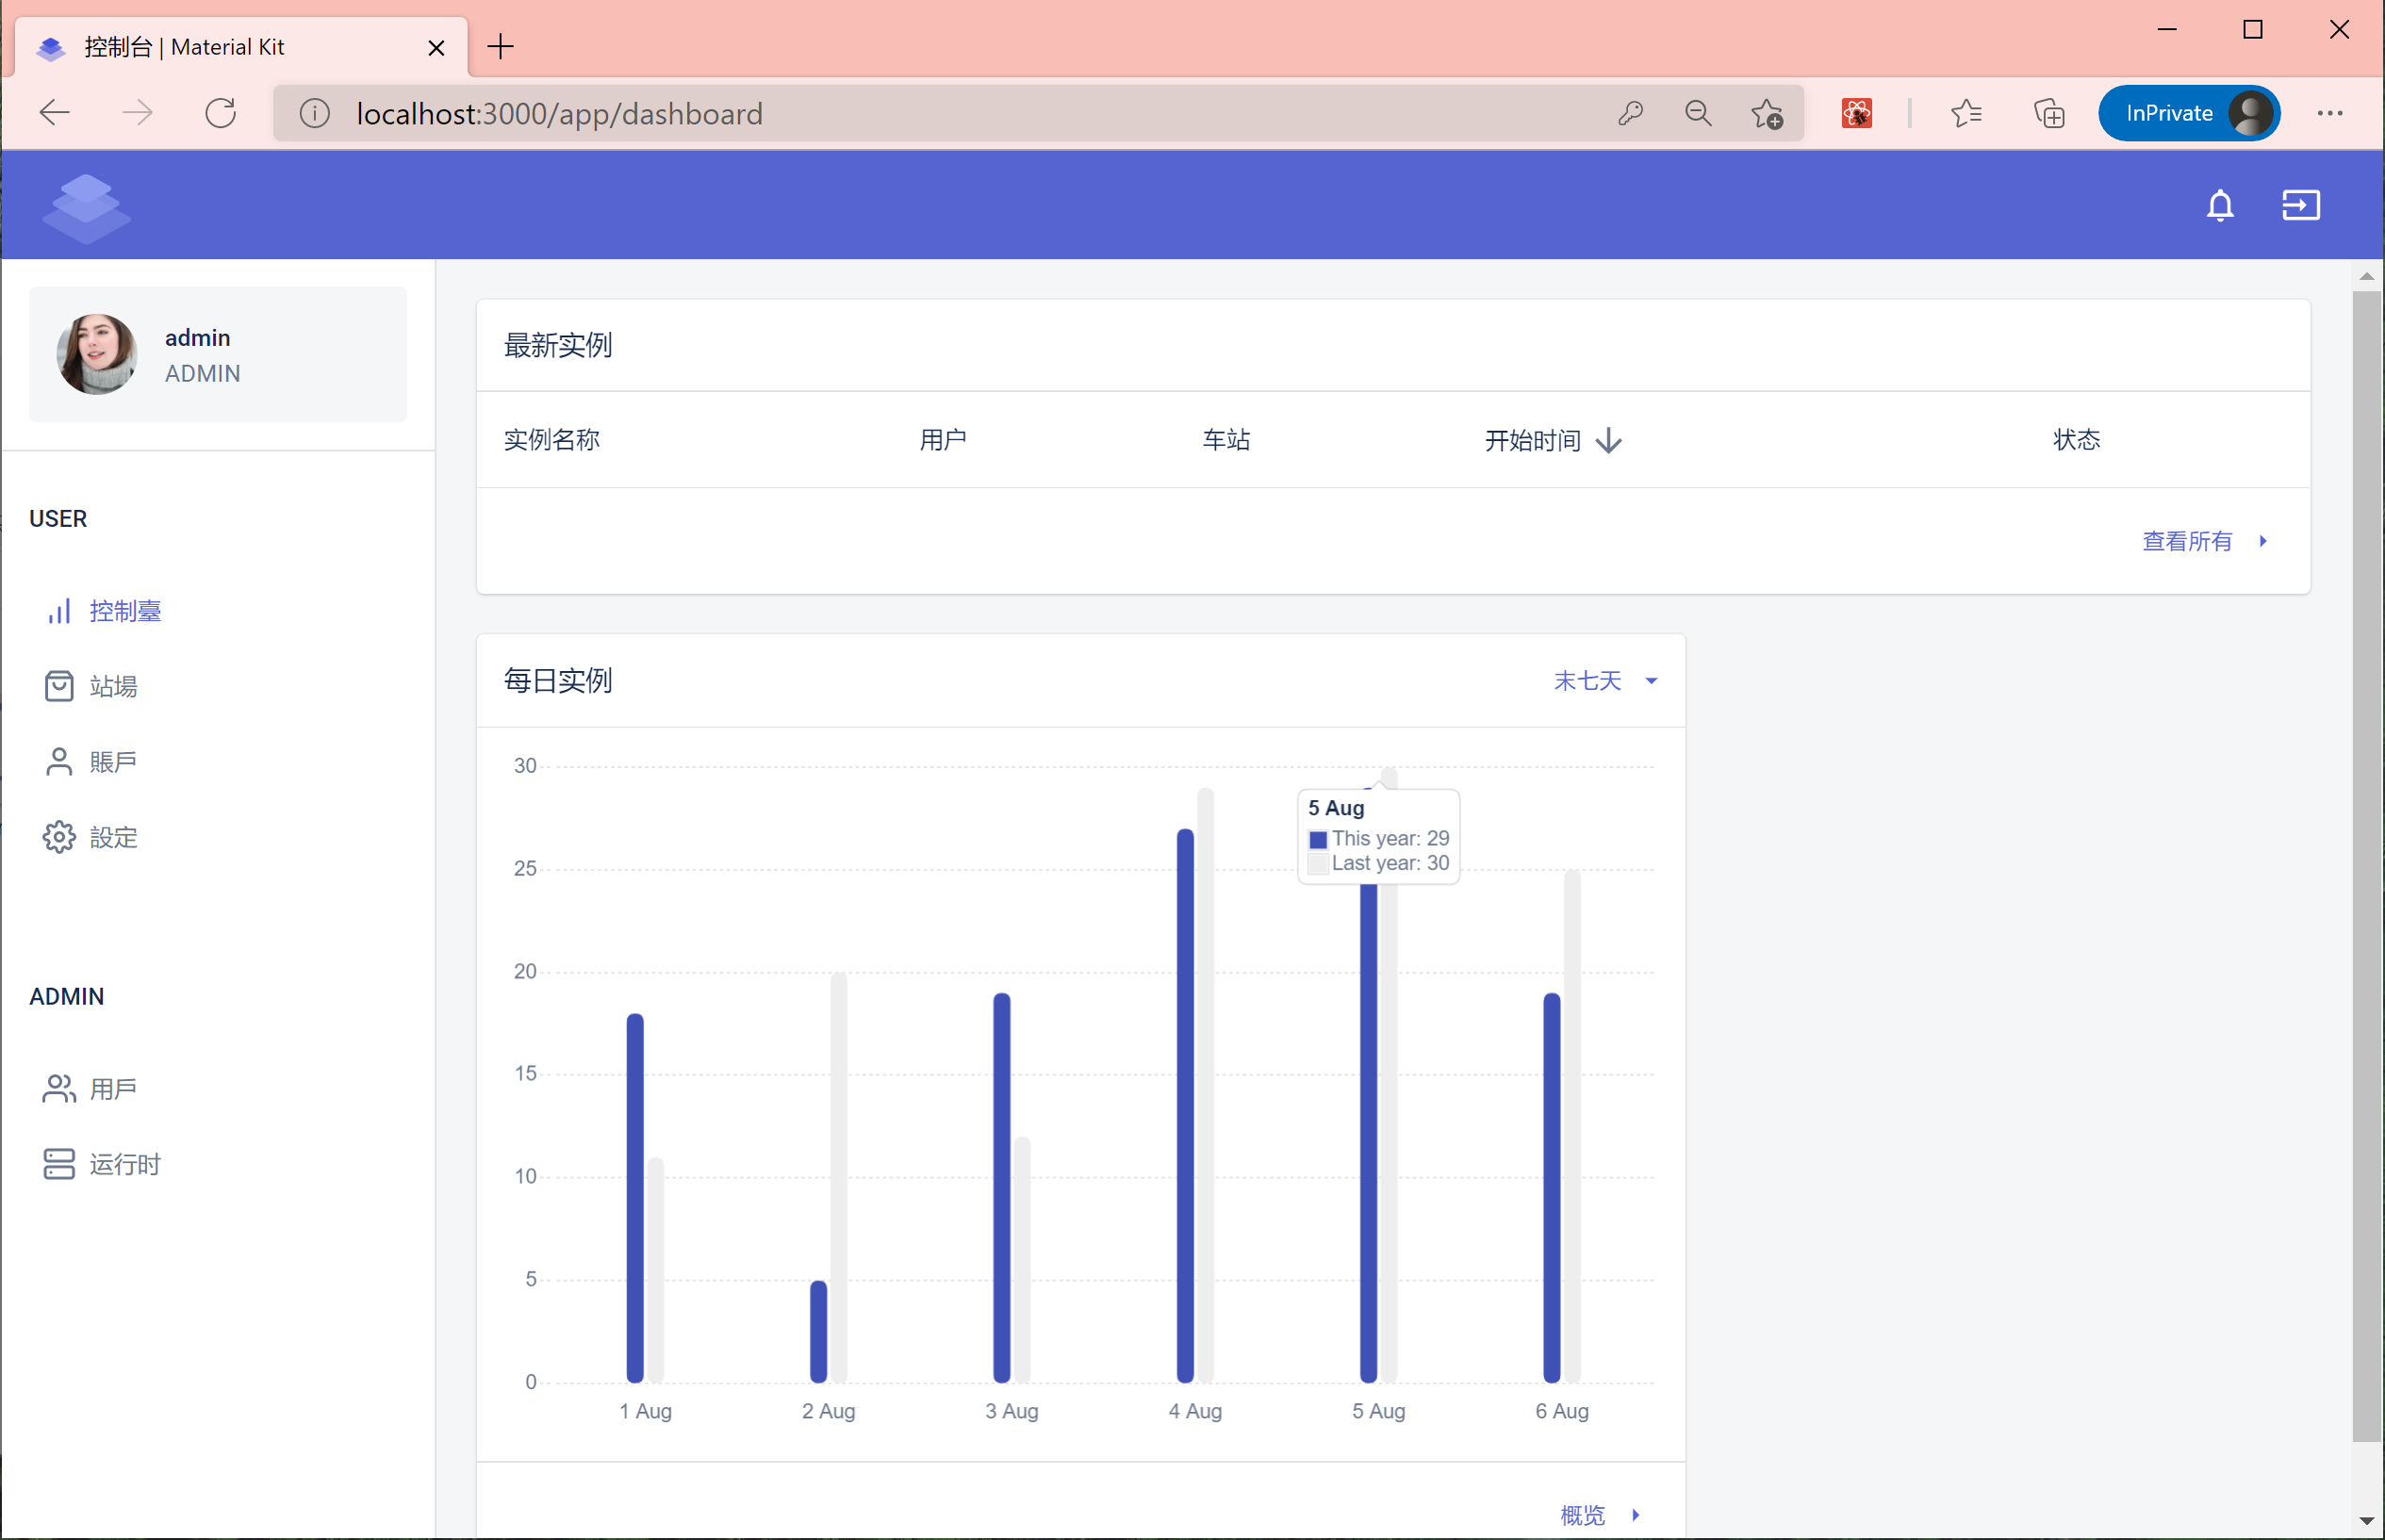
\includegraphics[width=\textwidth]{figures/png/admin_ui.png}
    \caption{\label{admin_ui}管理员角色的控制台首页}
\end{figure}

\begin{figure}[htbp!]
    \centering
    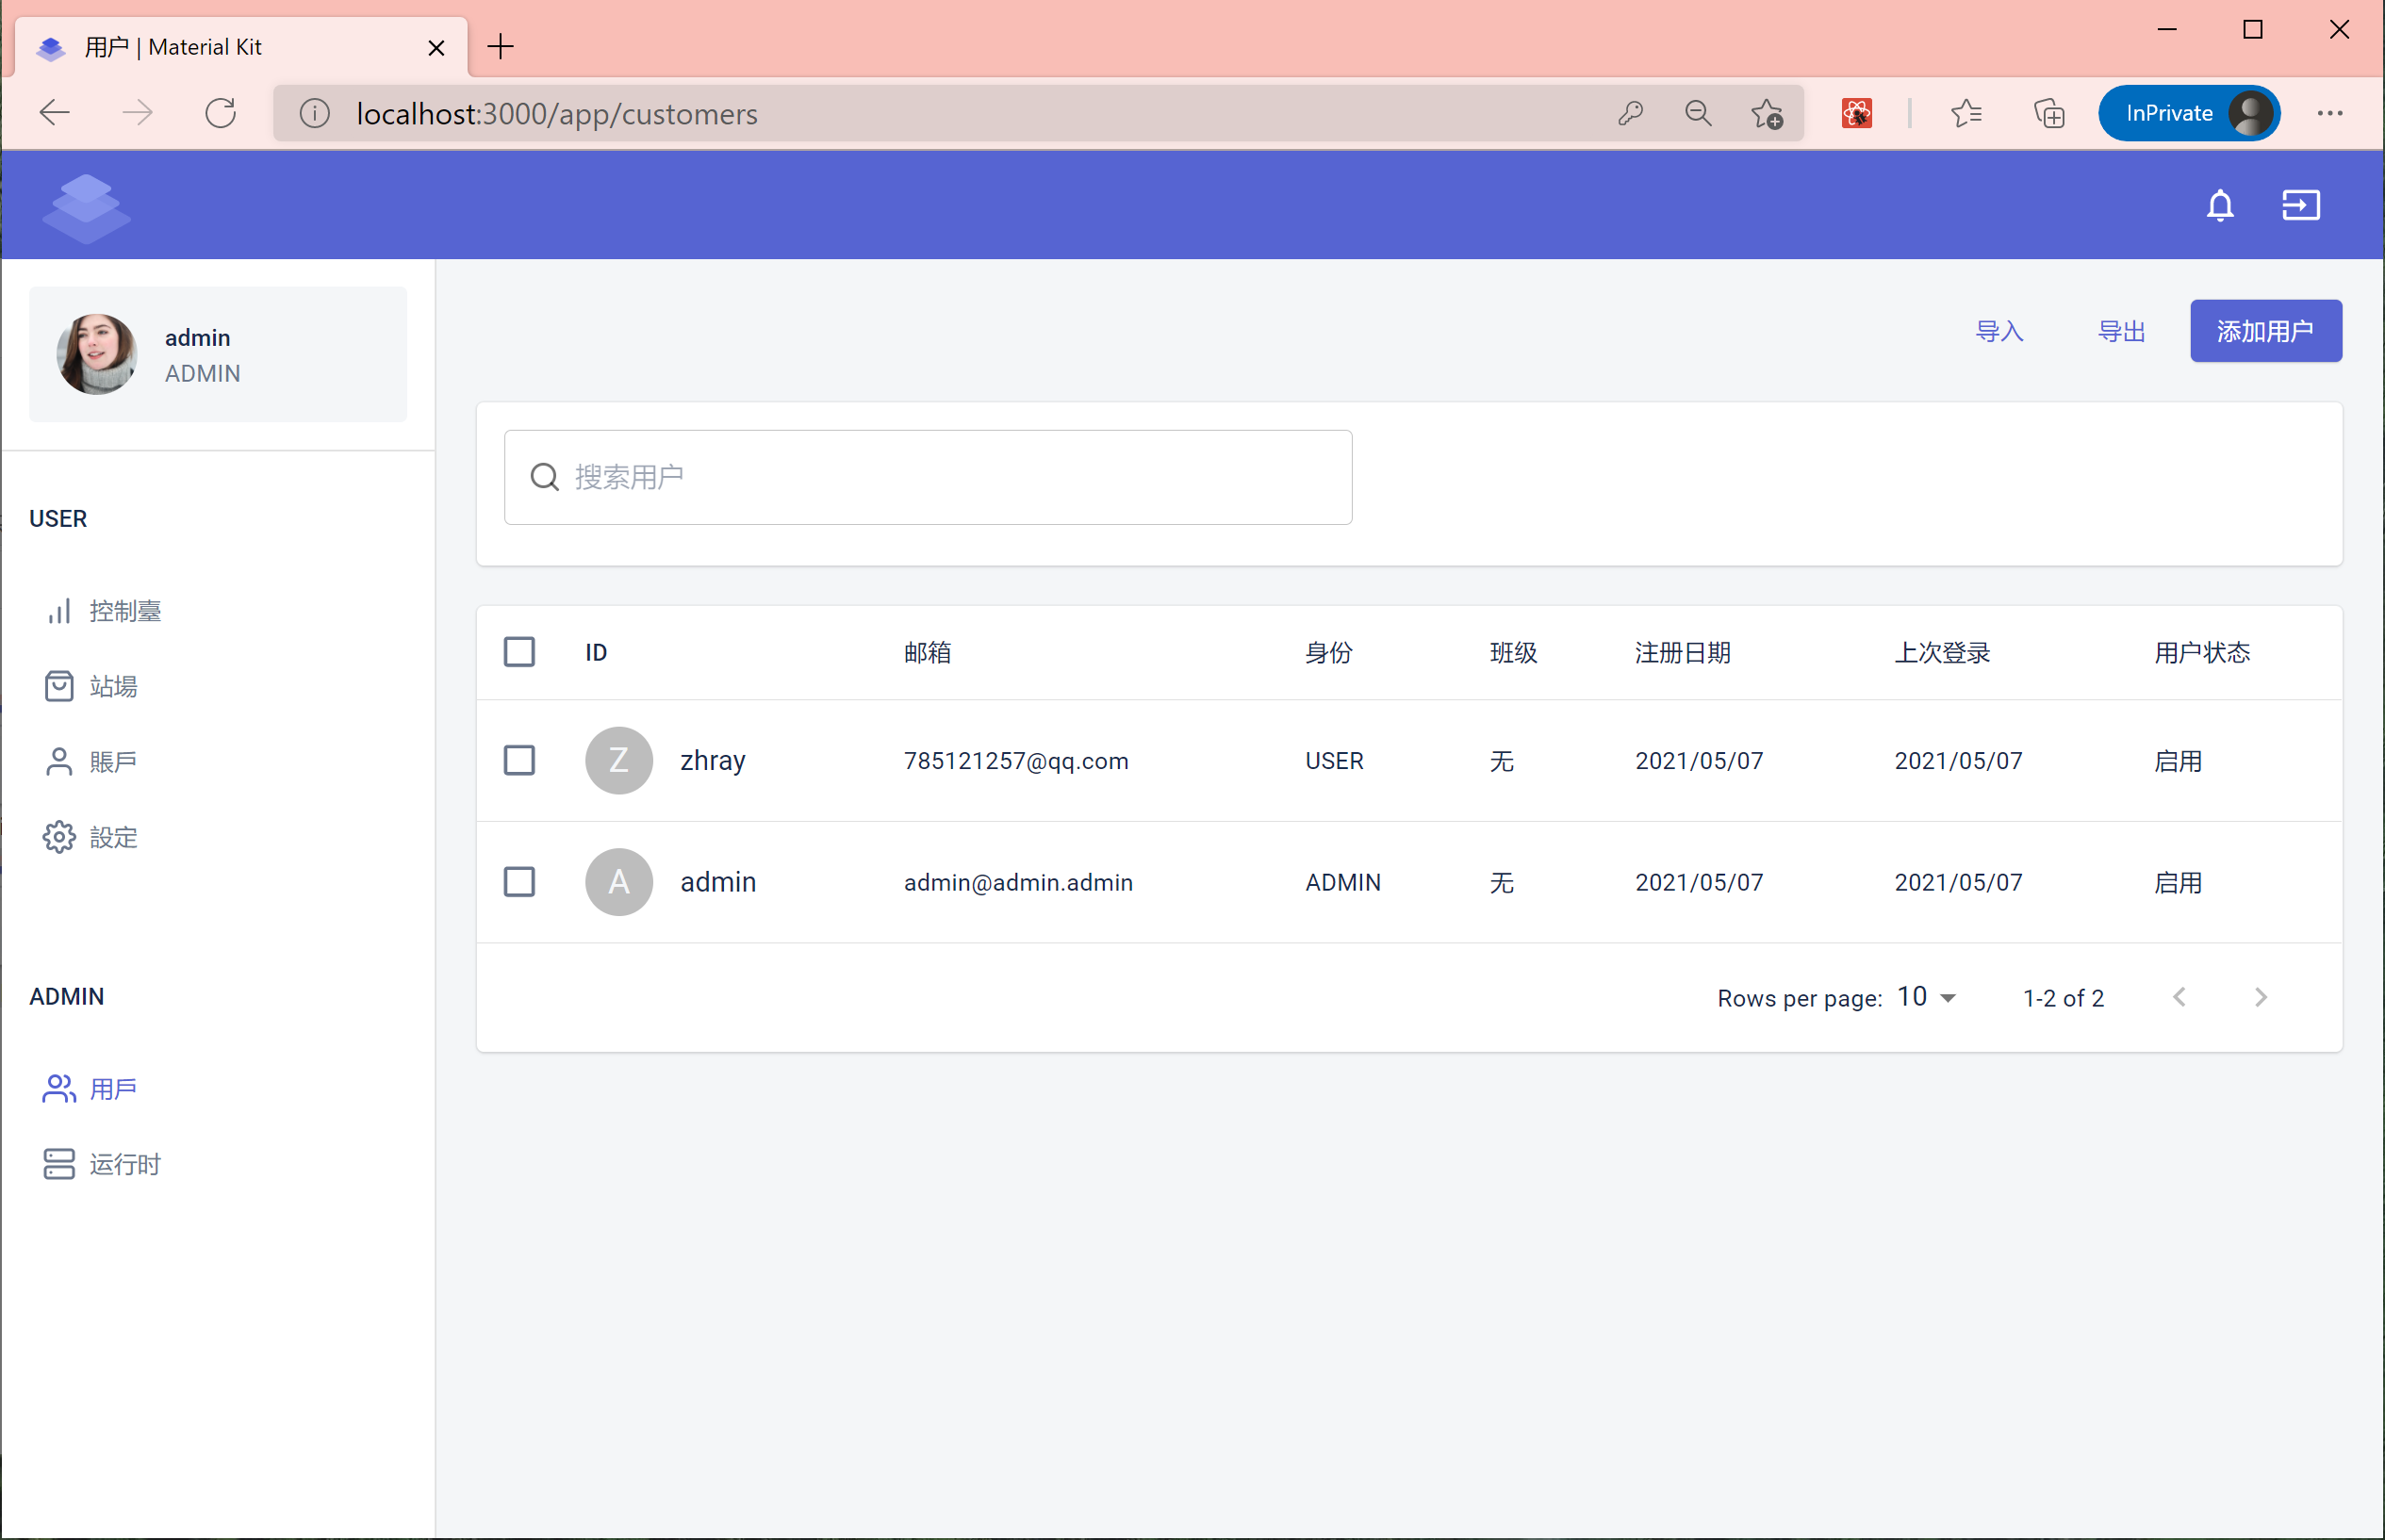
\includegraphics[width=\textwidth]{figures/png/admin_users.png}
    \caption{\label{admin_users}用户管理}
\end{figure}
\ref{admin_users} 可以看到刚刚注册成功的zhray账户。

\begin{figure}[htbp!]
    \centering
    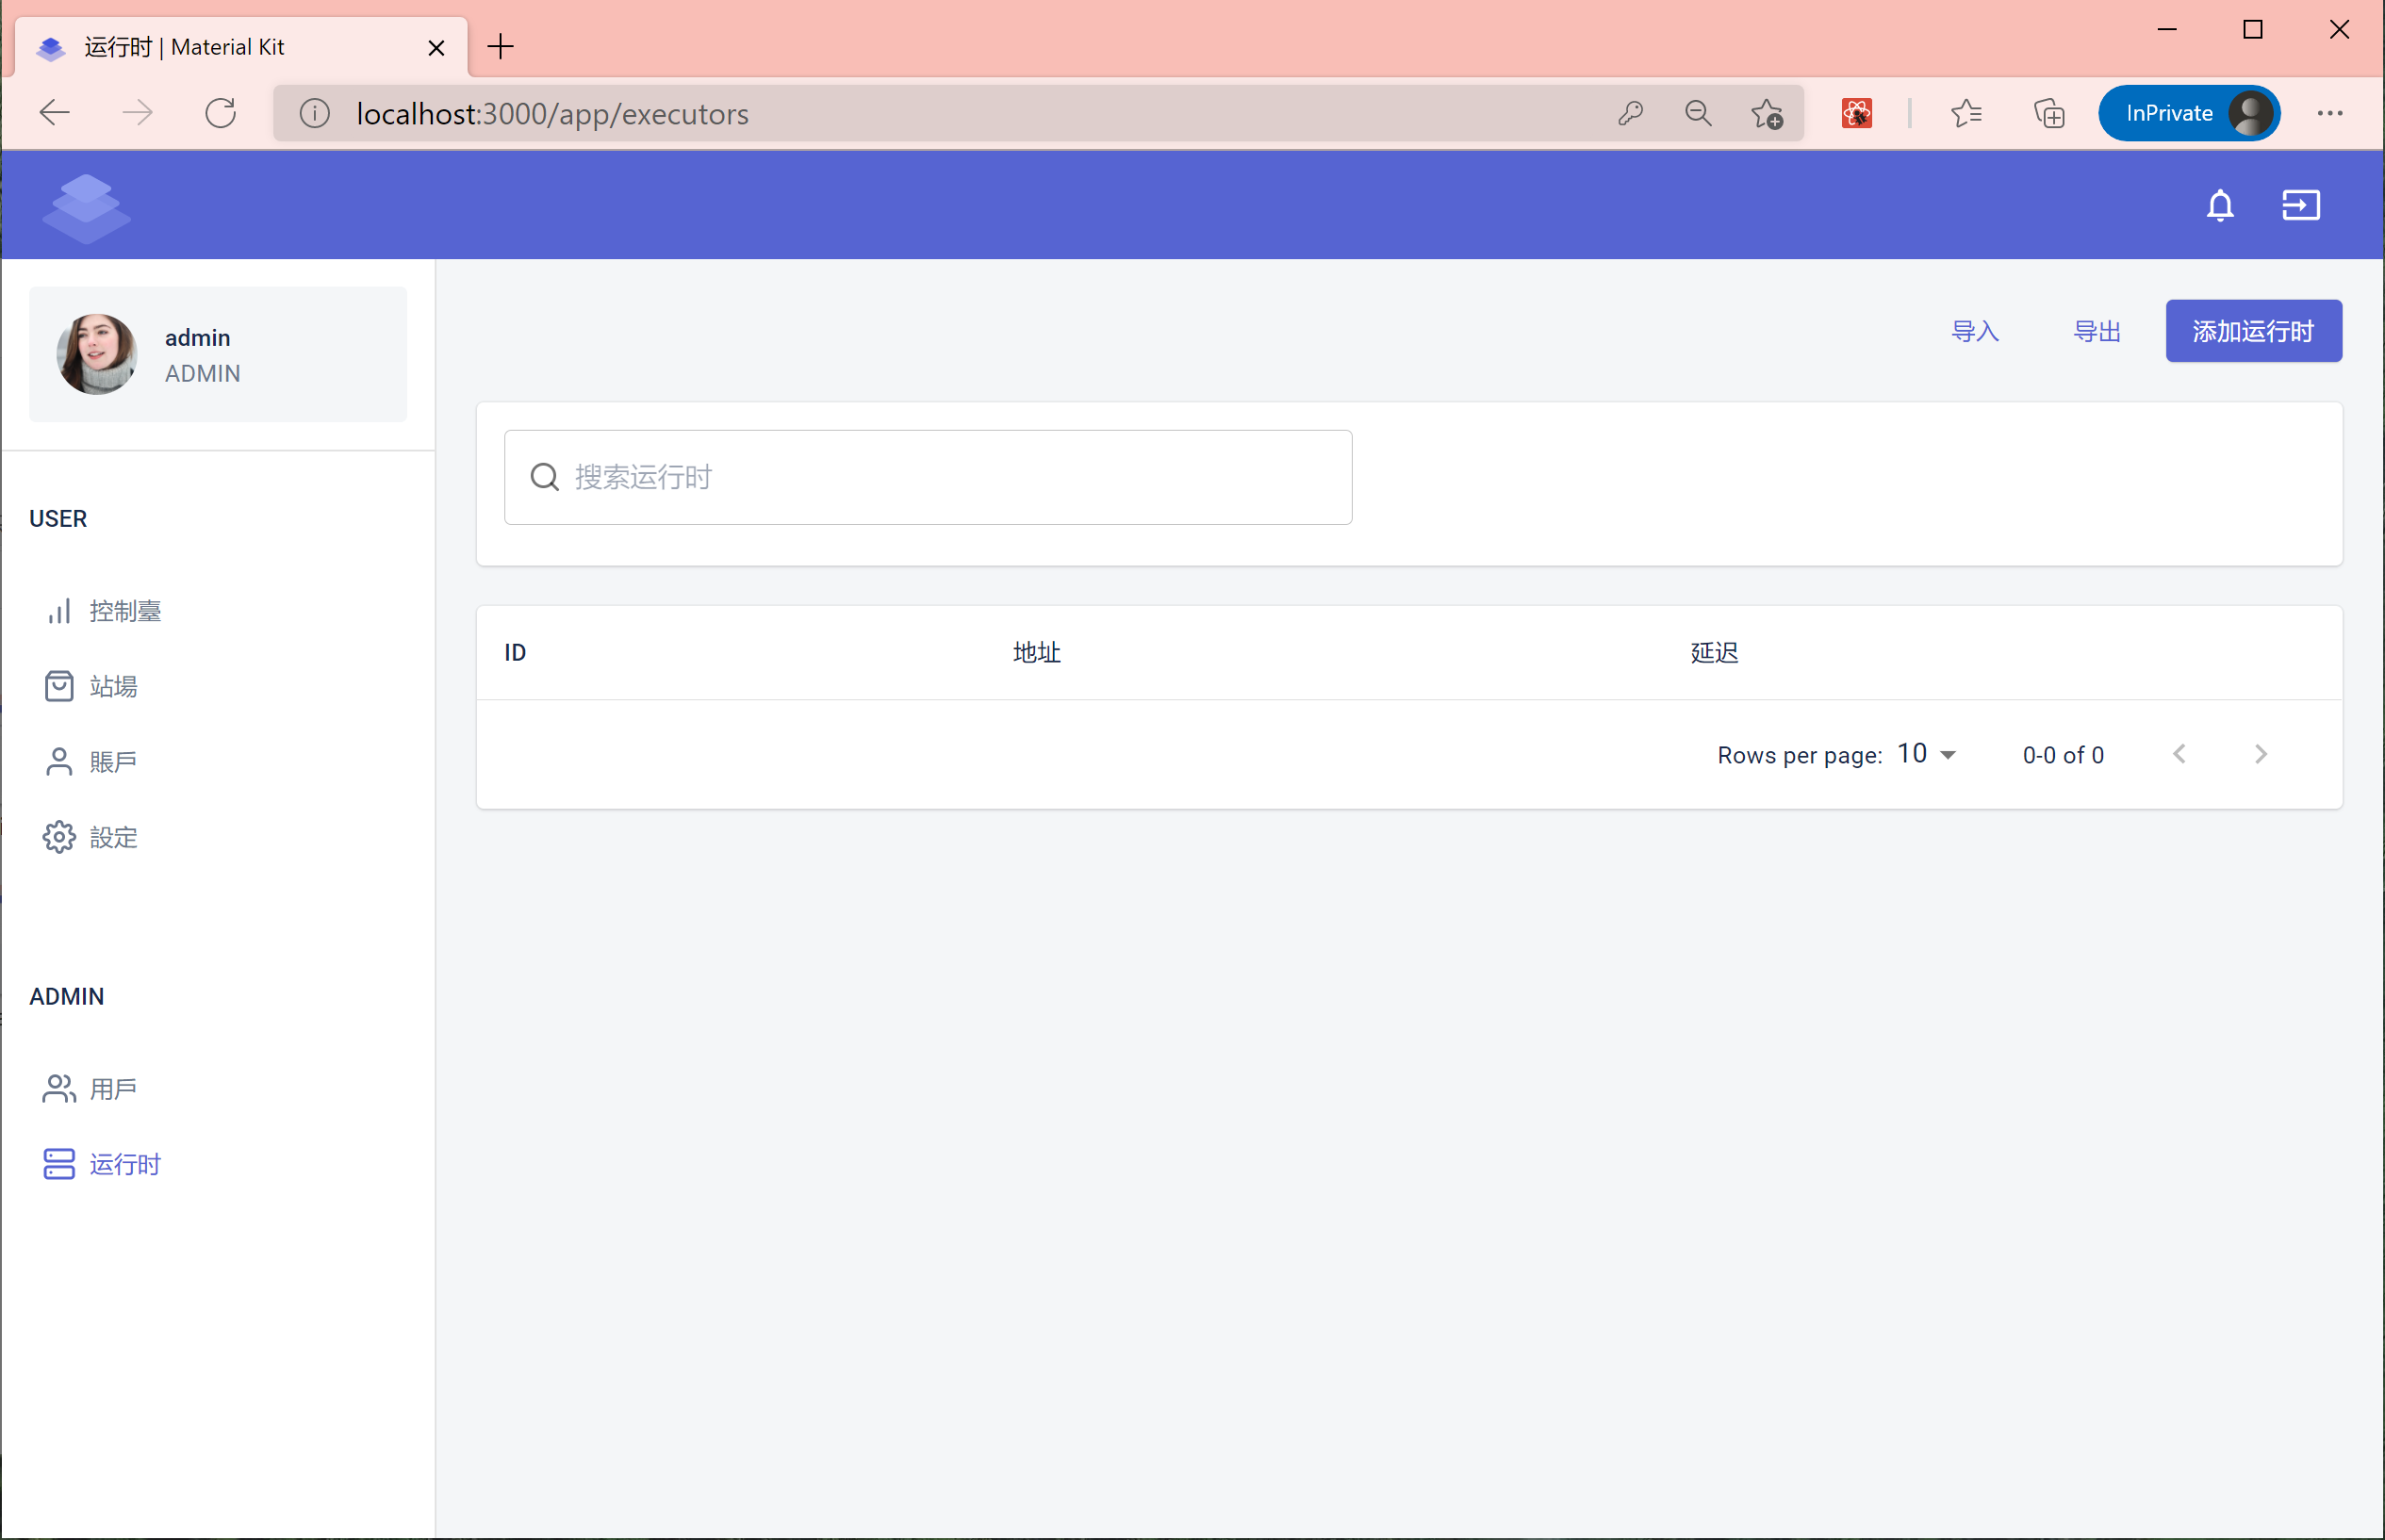
\includegraphics[width=\textwidth]{figures/png/exes.png}
    \caption{\label{exes}运行时管理}
\end{figure}

\begin{figure}[htbp!]
    \centering
    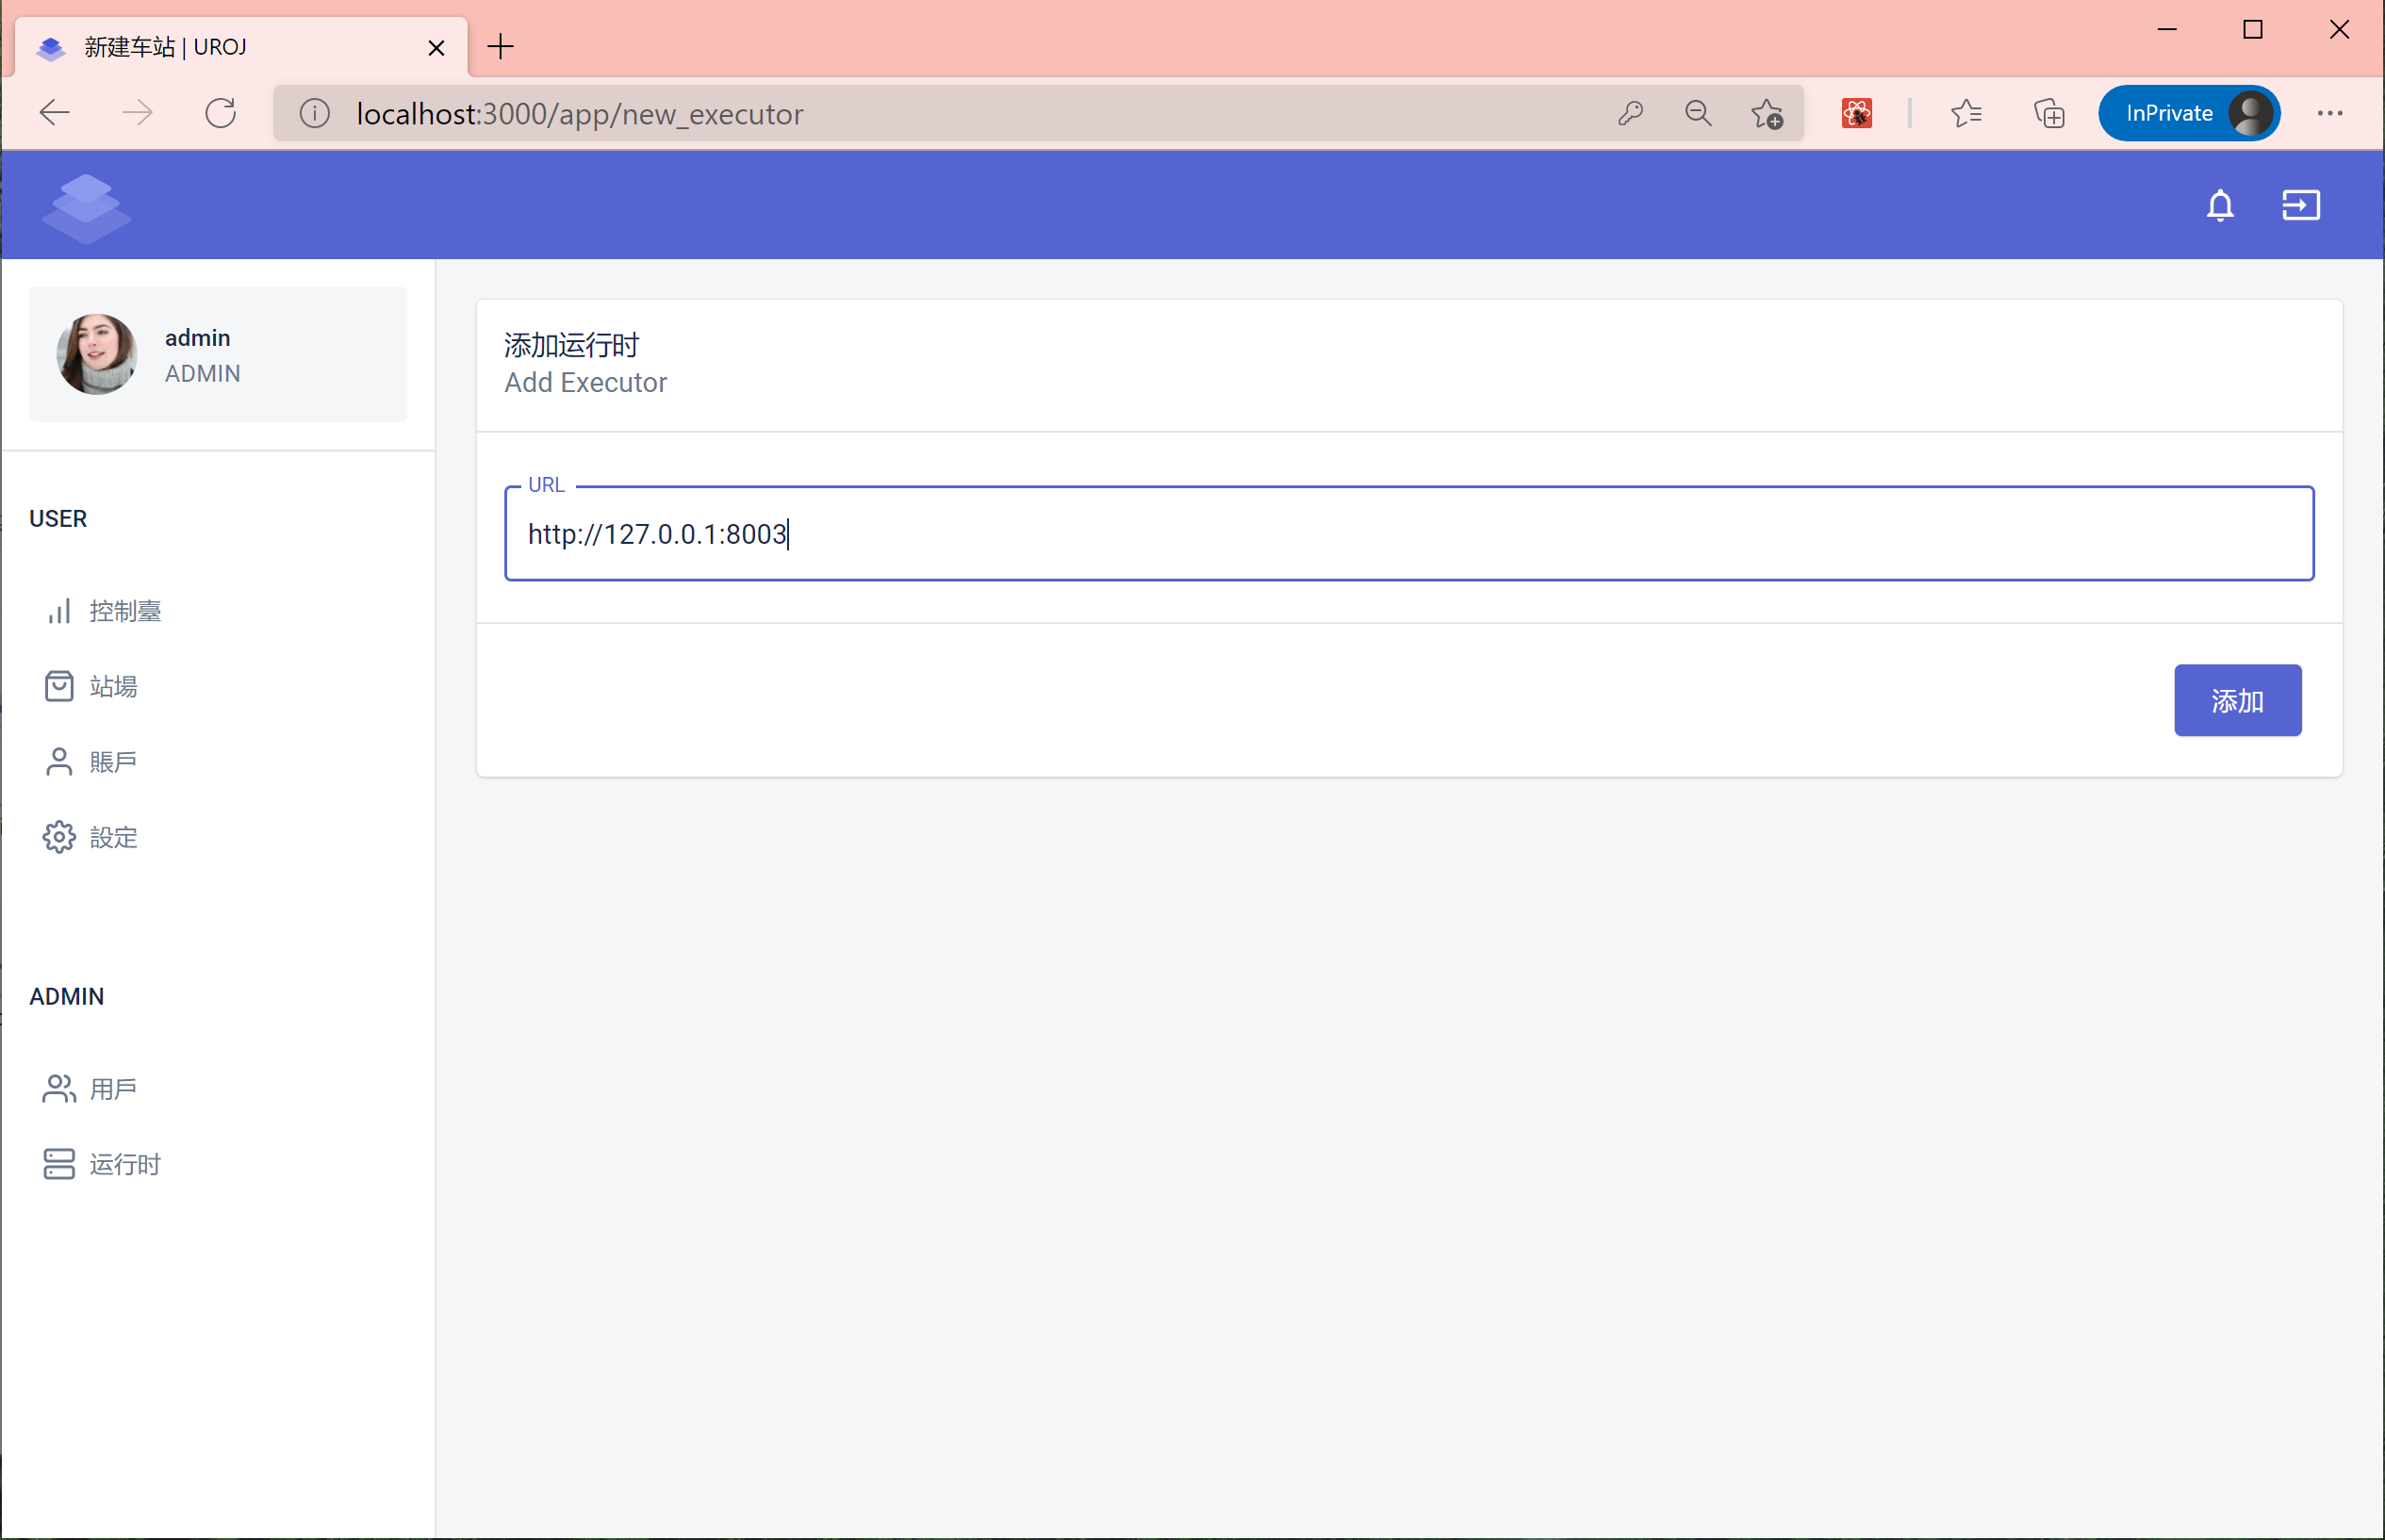
\includegraphics[width=\textwidth]{figures/png/add_exes.png}
    \caption{\label{add_exes}添加运行时}
\end{figure}

\begin{figure}[htbp!]
    \centering
    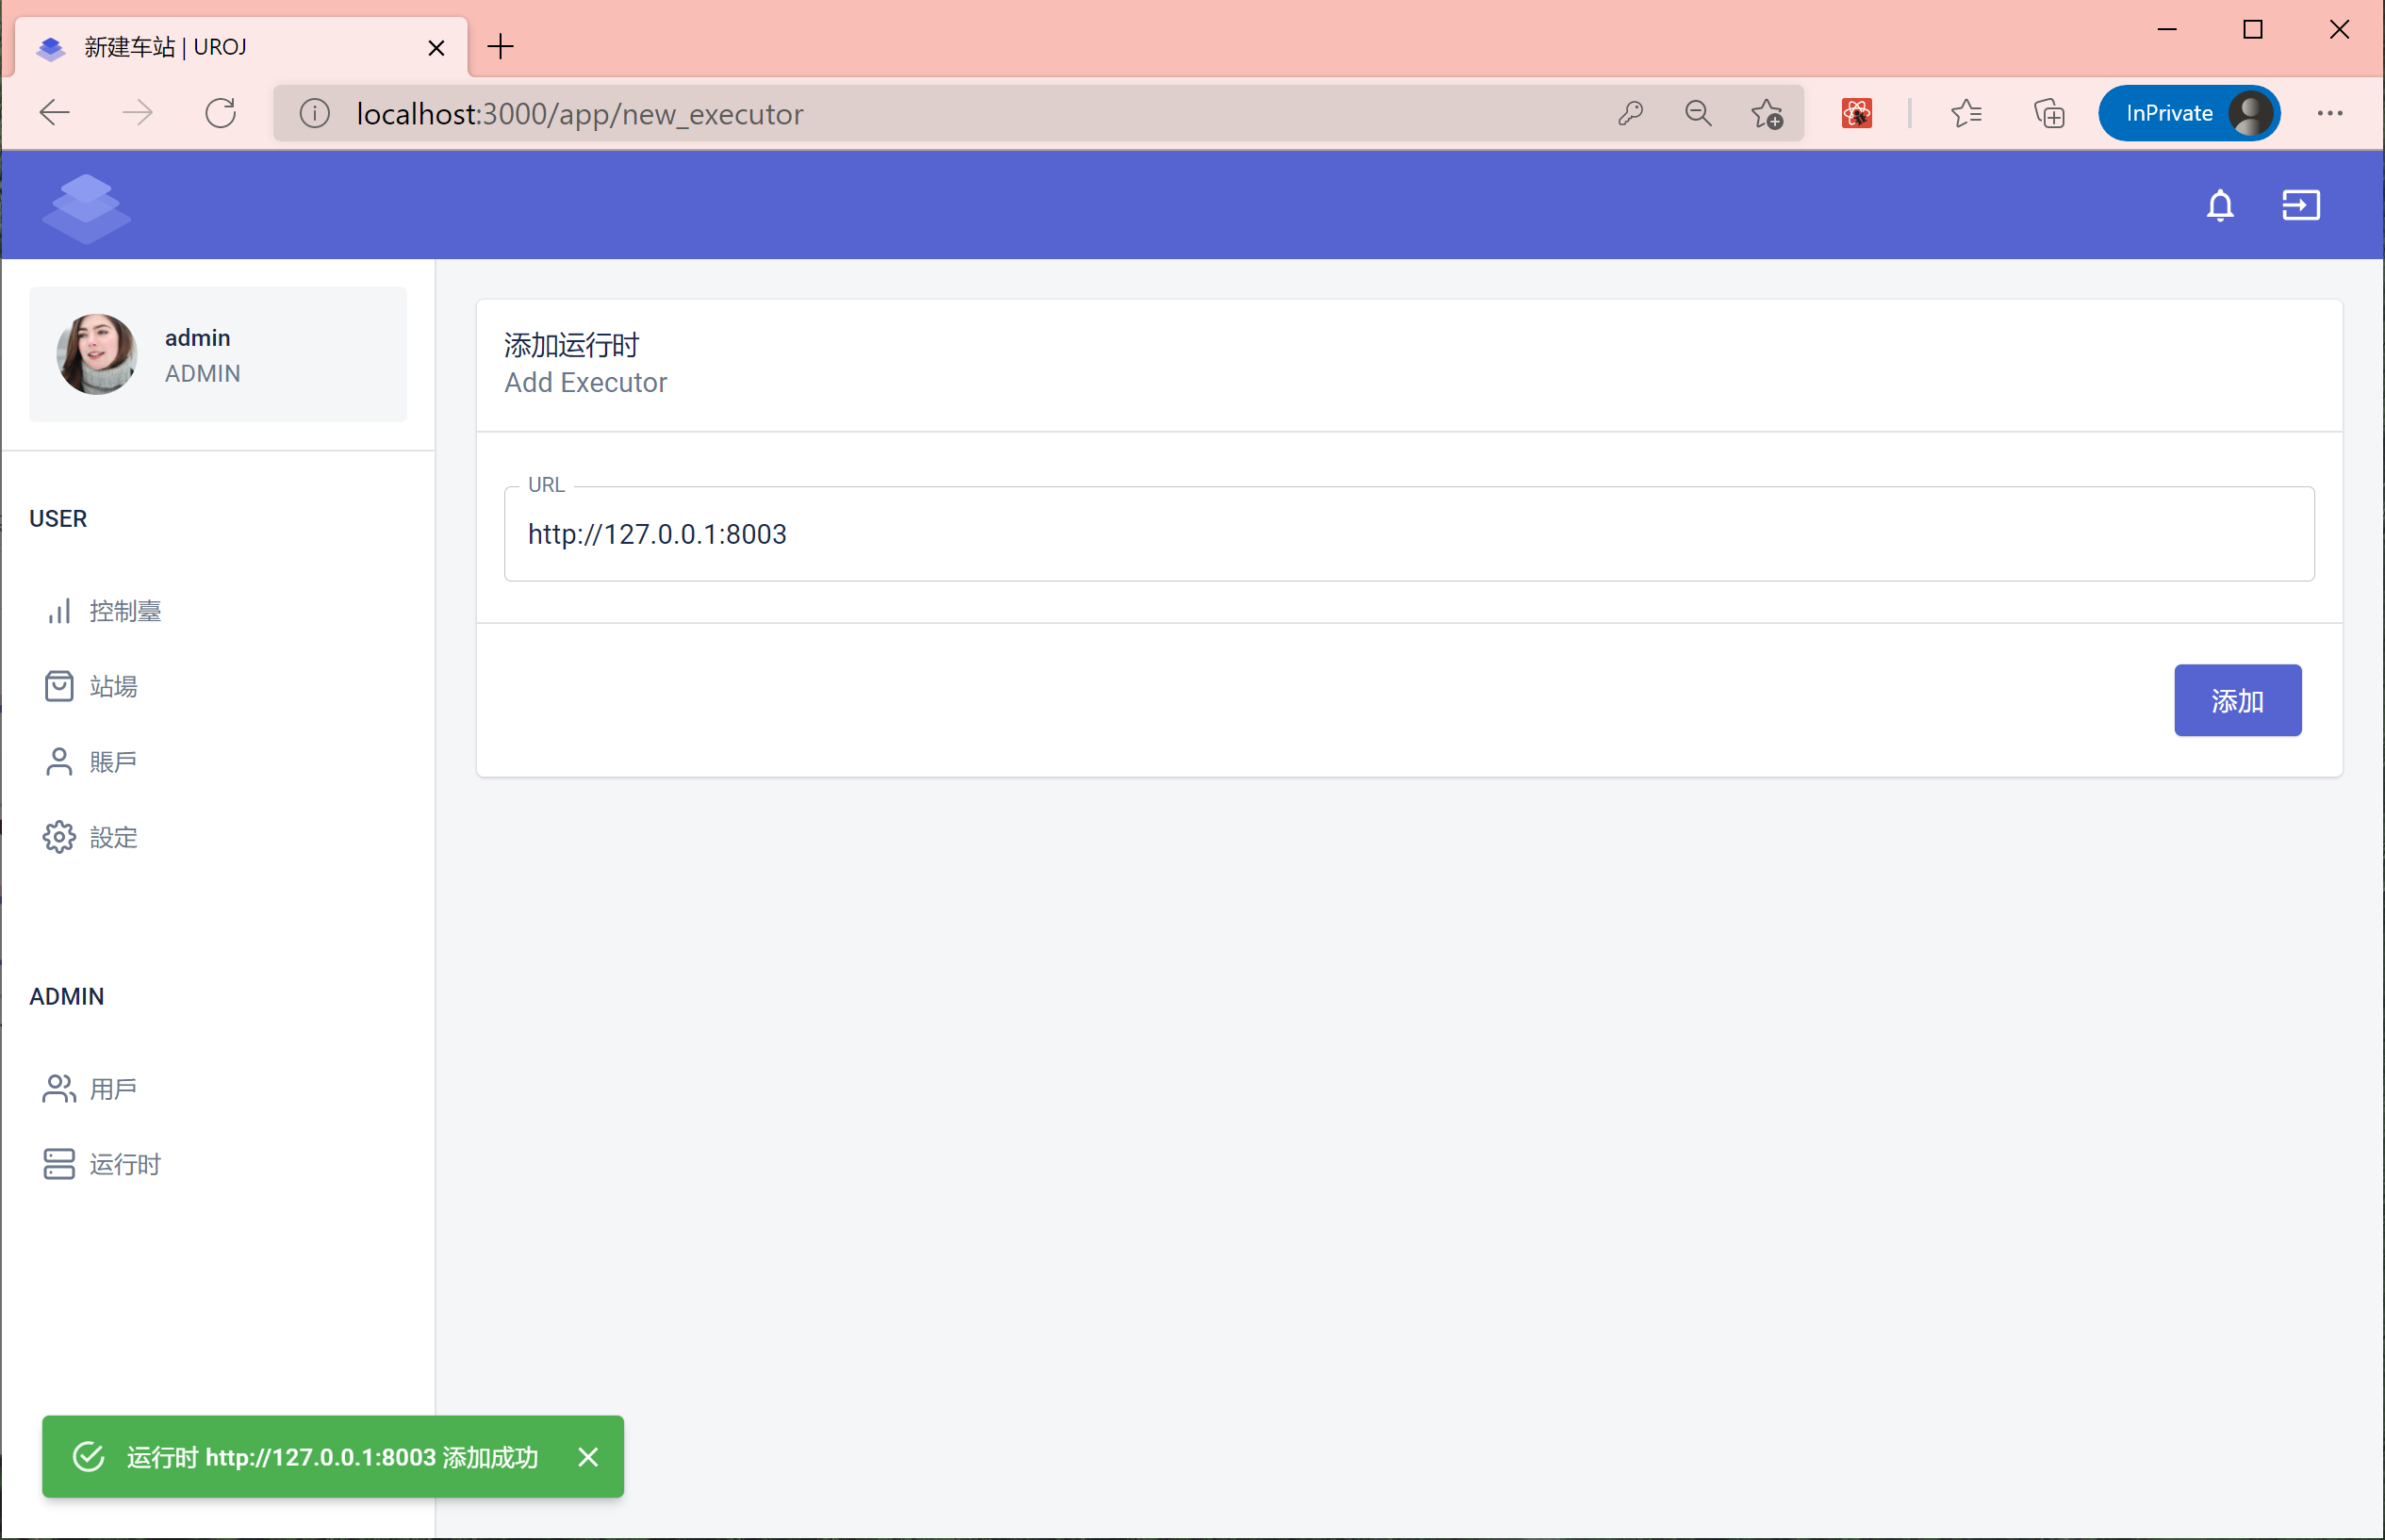
\includegraphics[width=\textwidth]{figures/png/add_exe_succ.png}
    \caption{\label{add_exe_succ}添加运行时成功}
\end{figure}

\begin{figure}[htbp!]
    \centering
    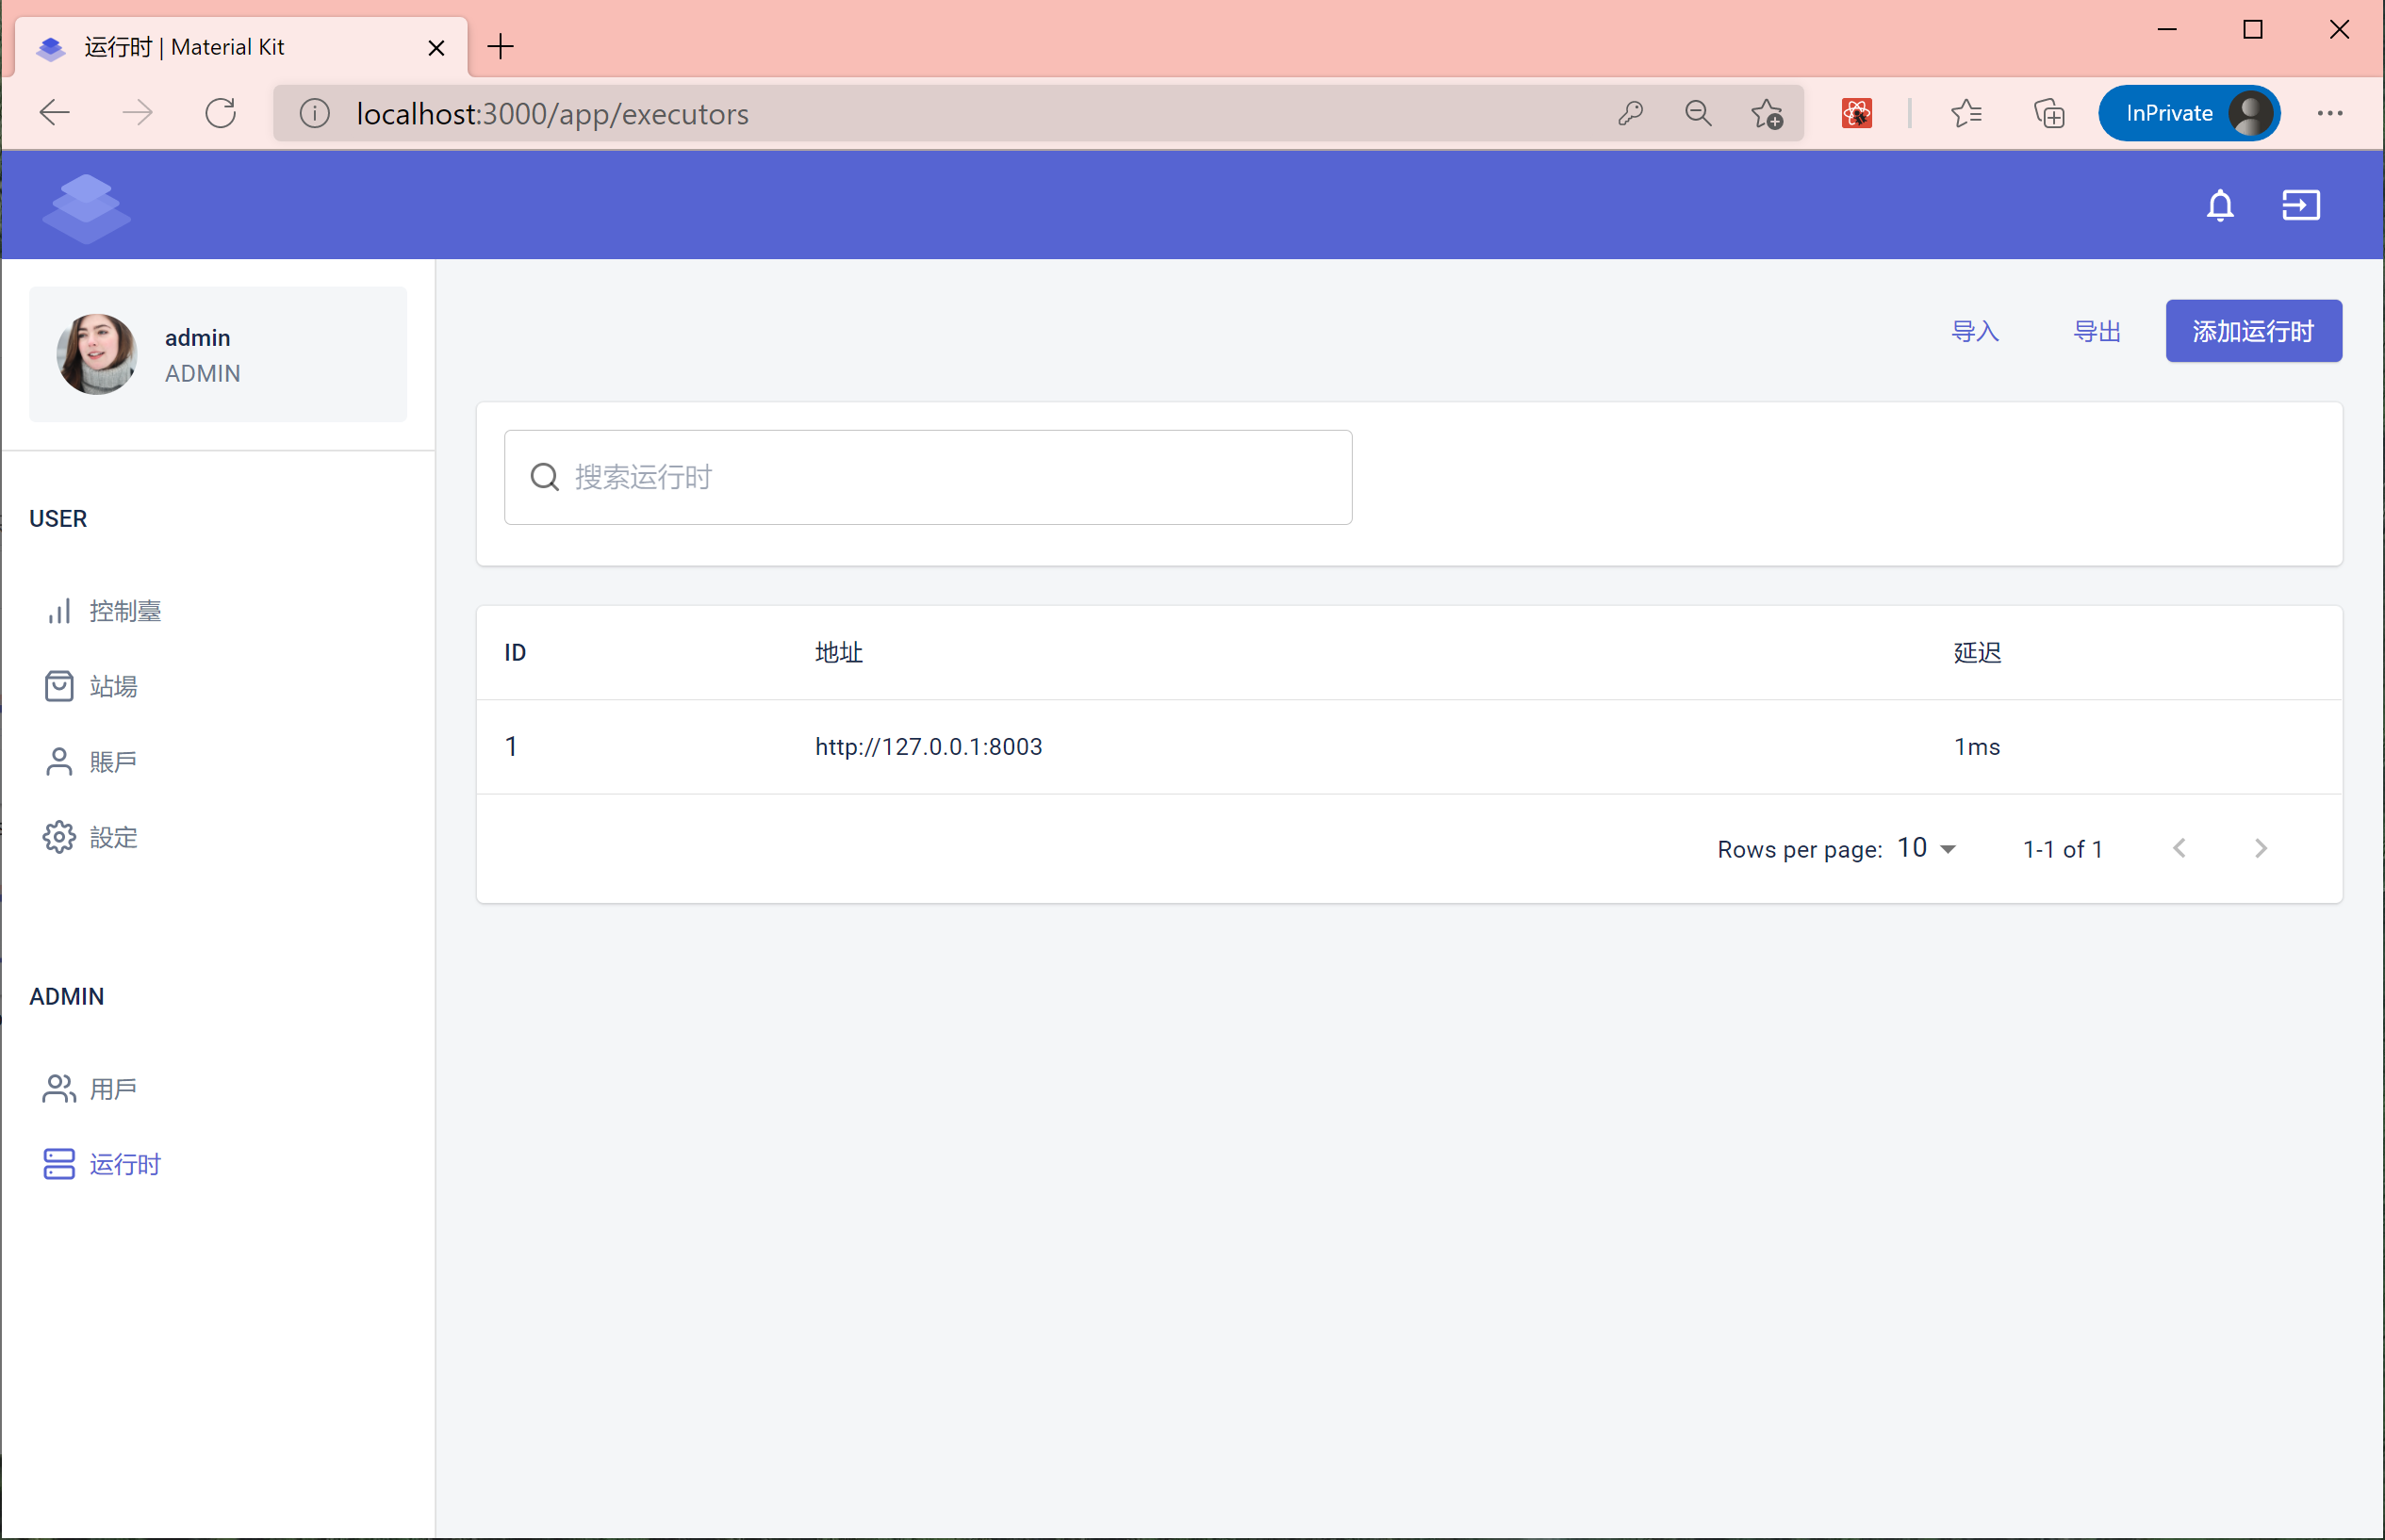
\includegraphics[width=\textwidth]{figures/png/new_exes.png}
    \caption{\label{new_exes}刚刚新添加的运行时}
\end{figure}

\begin{figure}[htbp!]
    \centering
    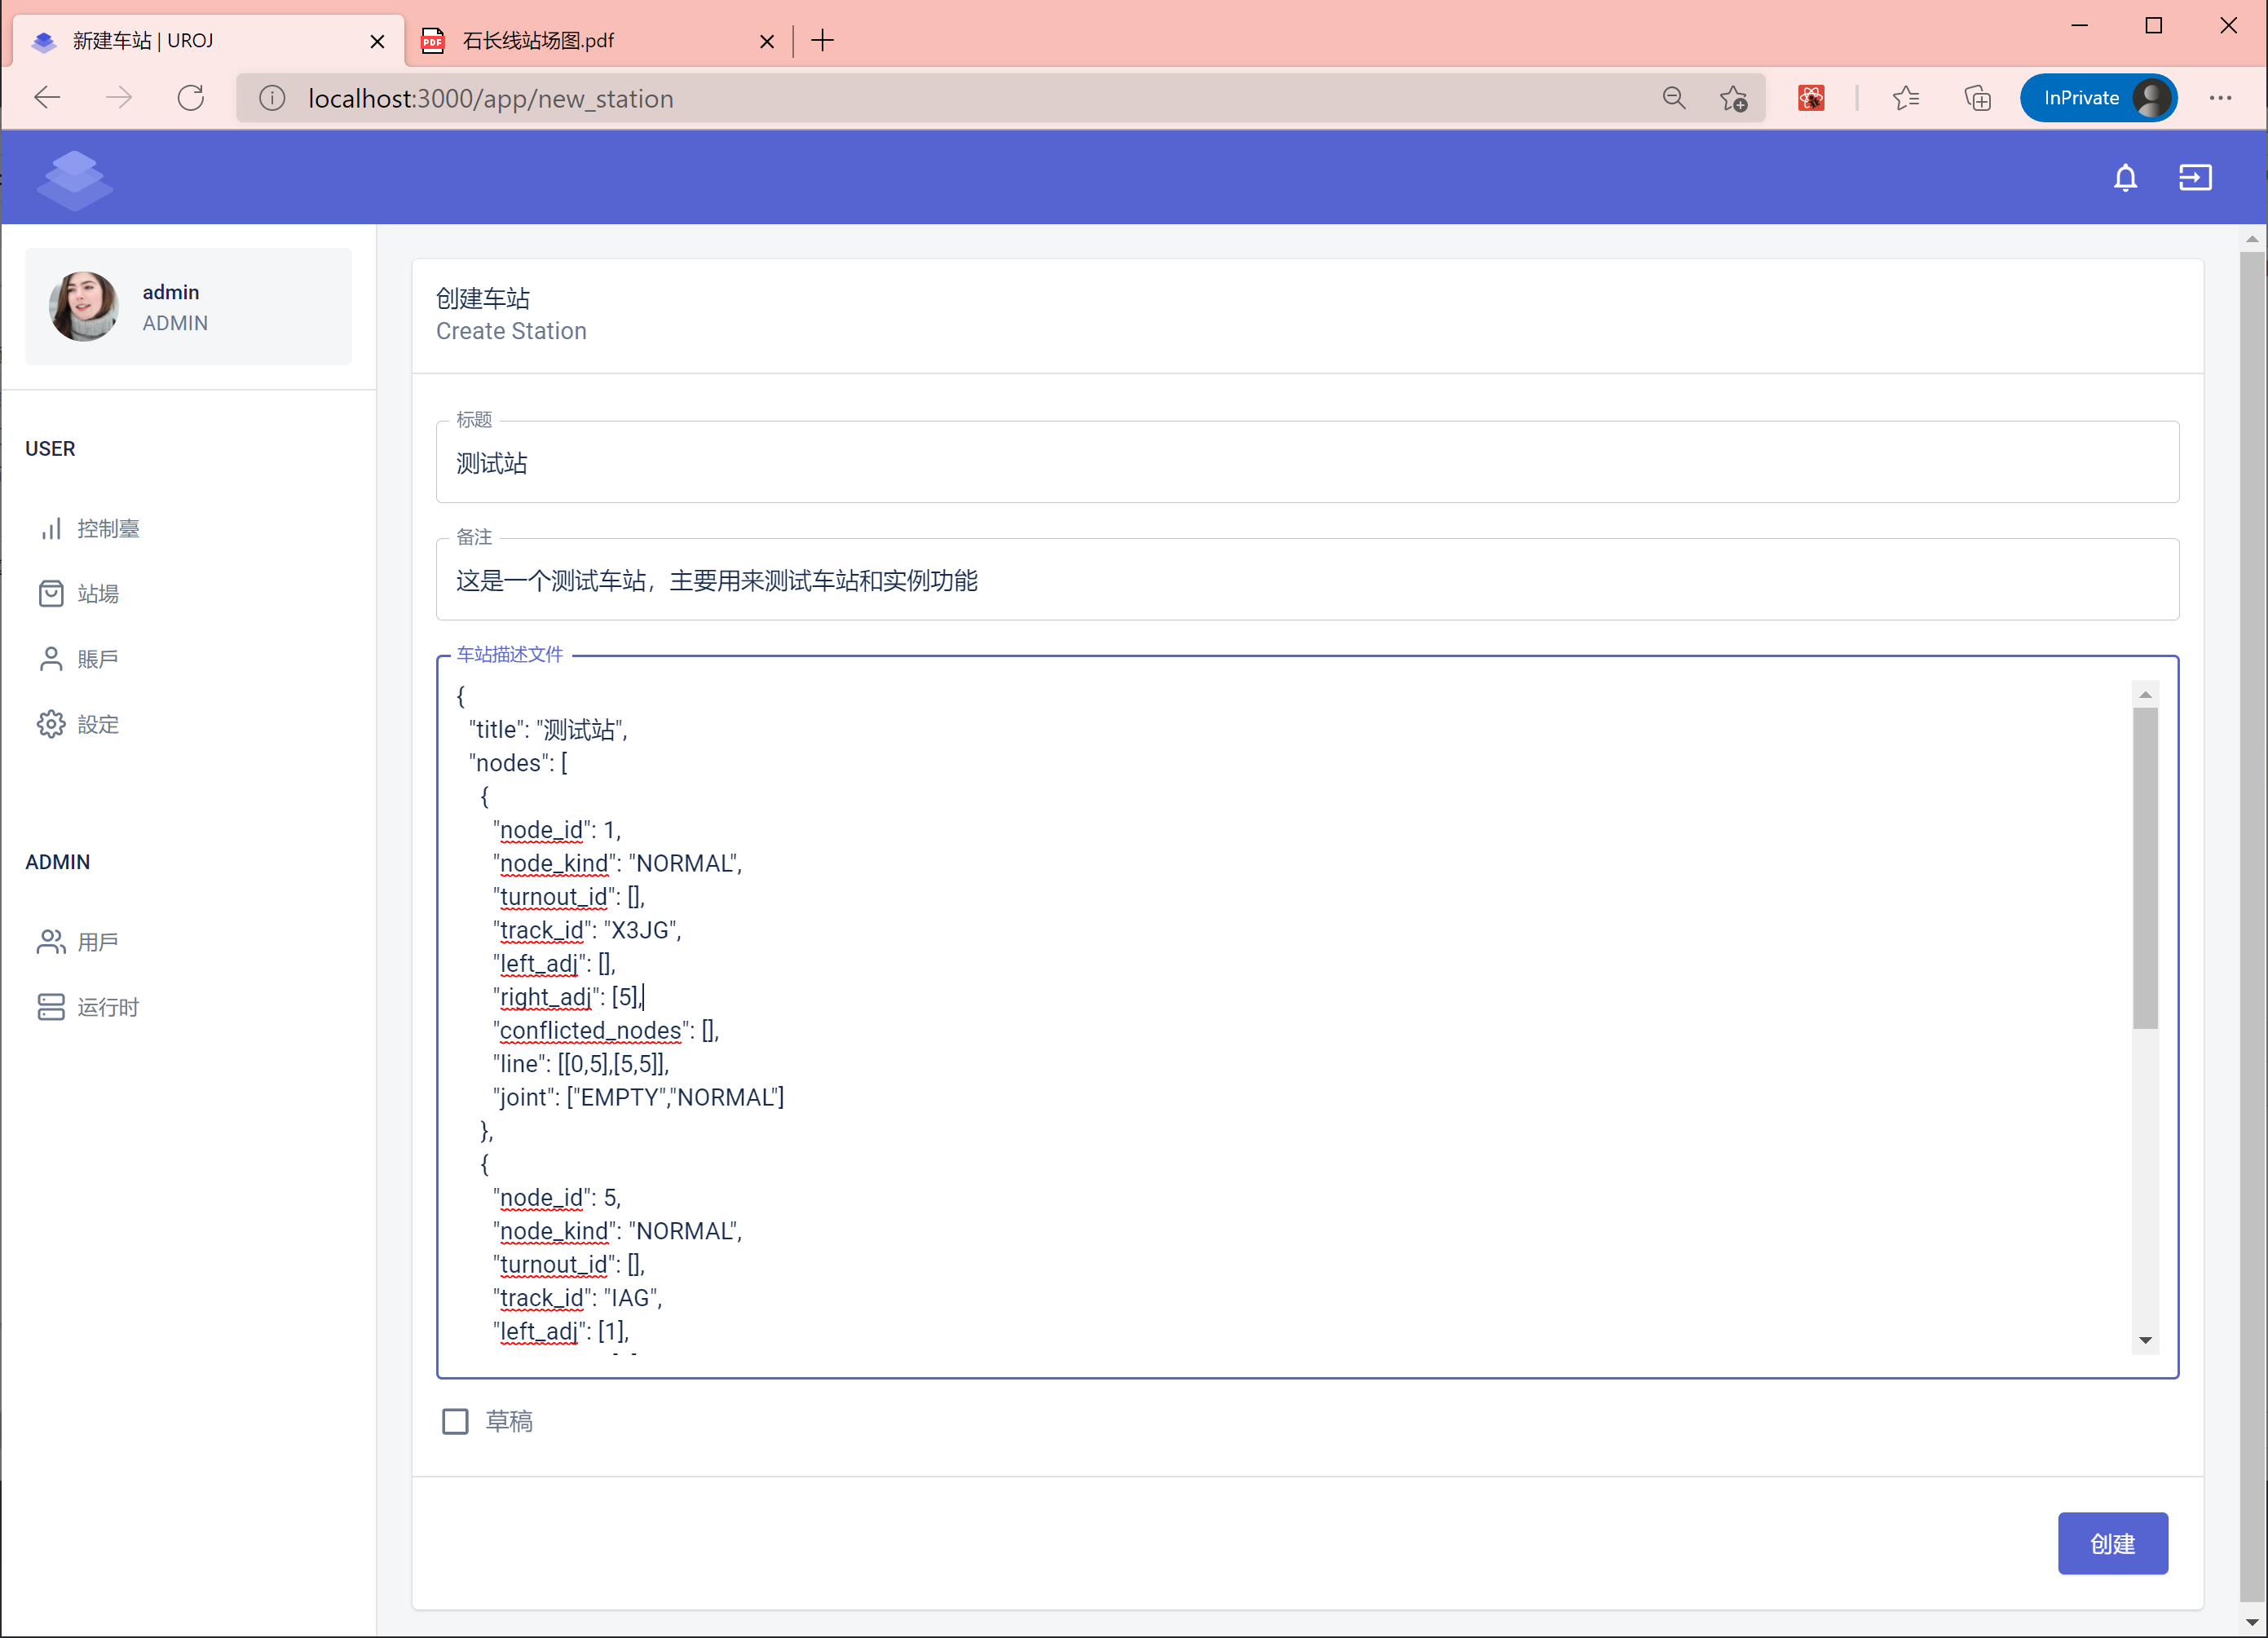
\includegraphics[width=\textwidth]{figures/png/create_sta.png}
    \caption{\label{create_sta}创建车站}
\end{figure}

\begin{figure}[htbp!]
    \centering
    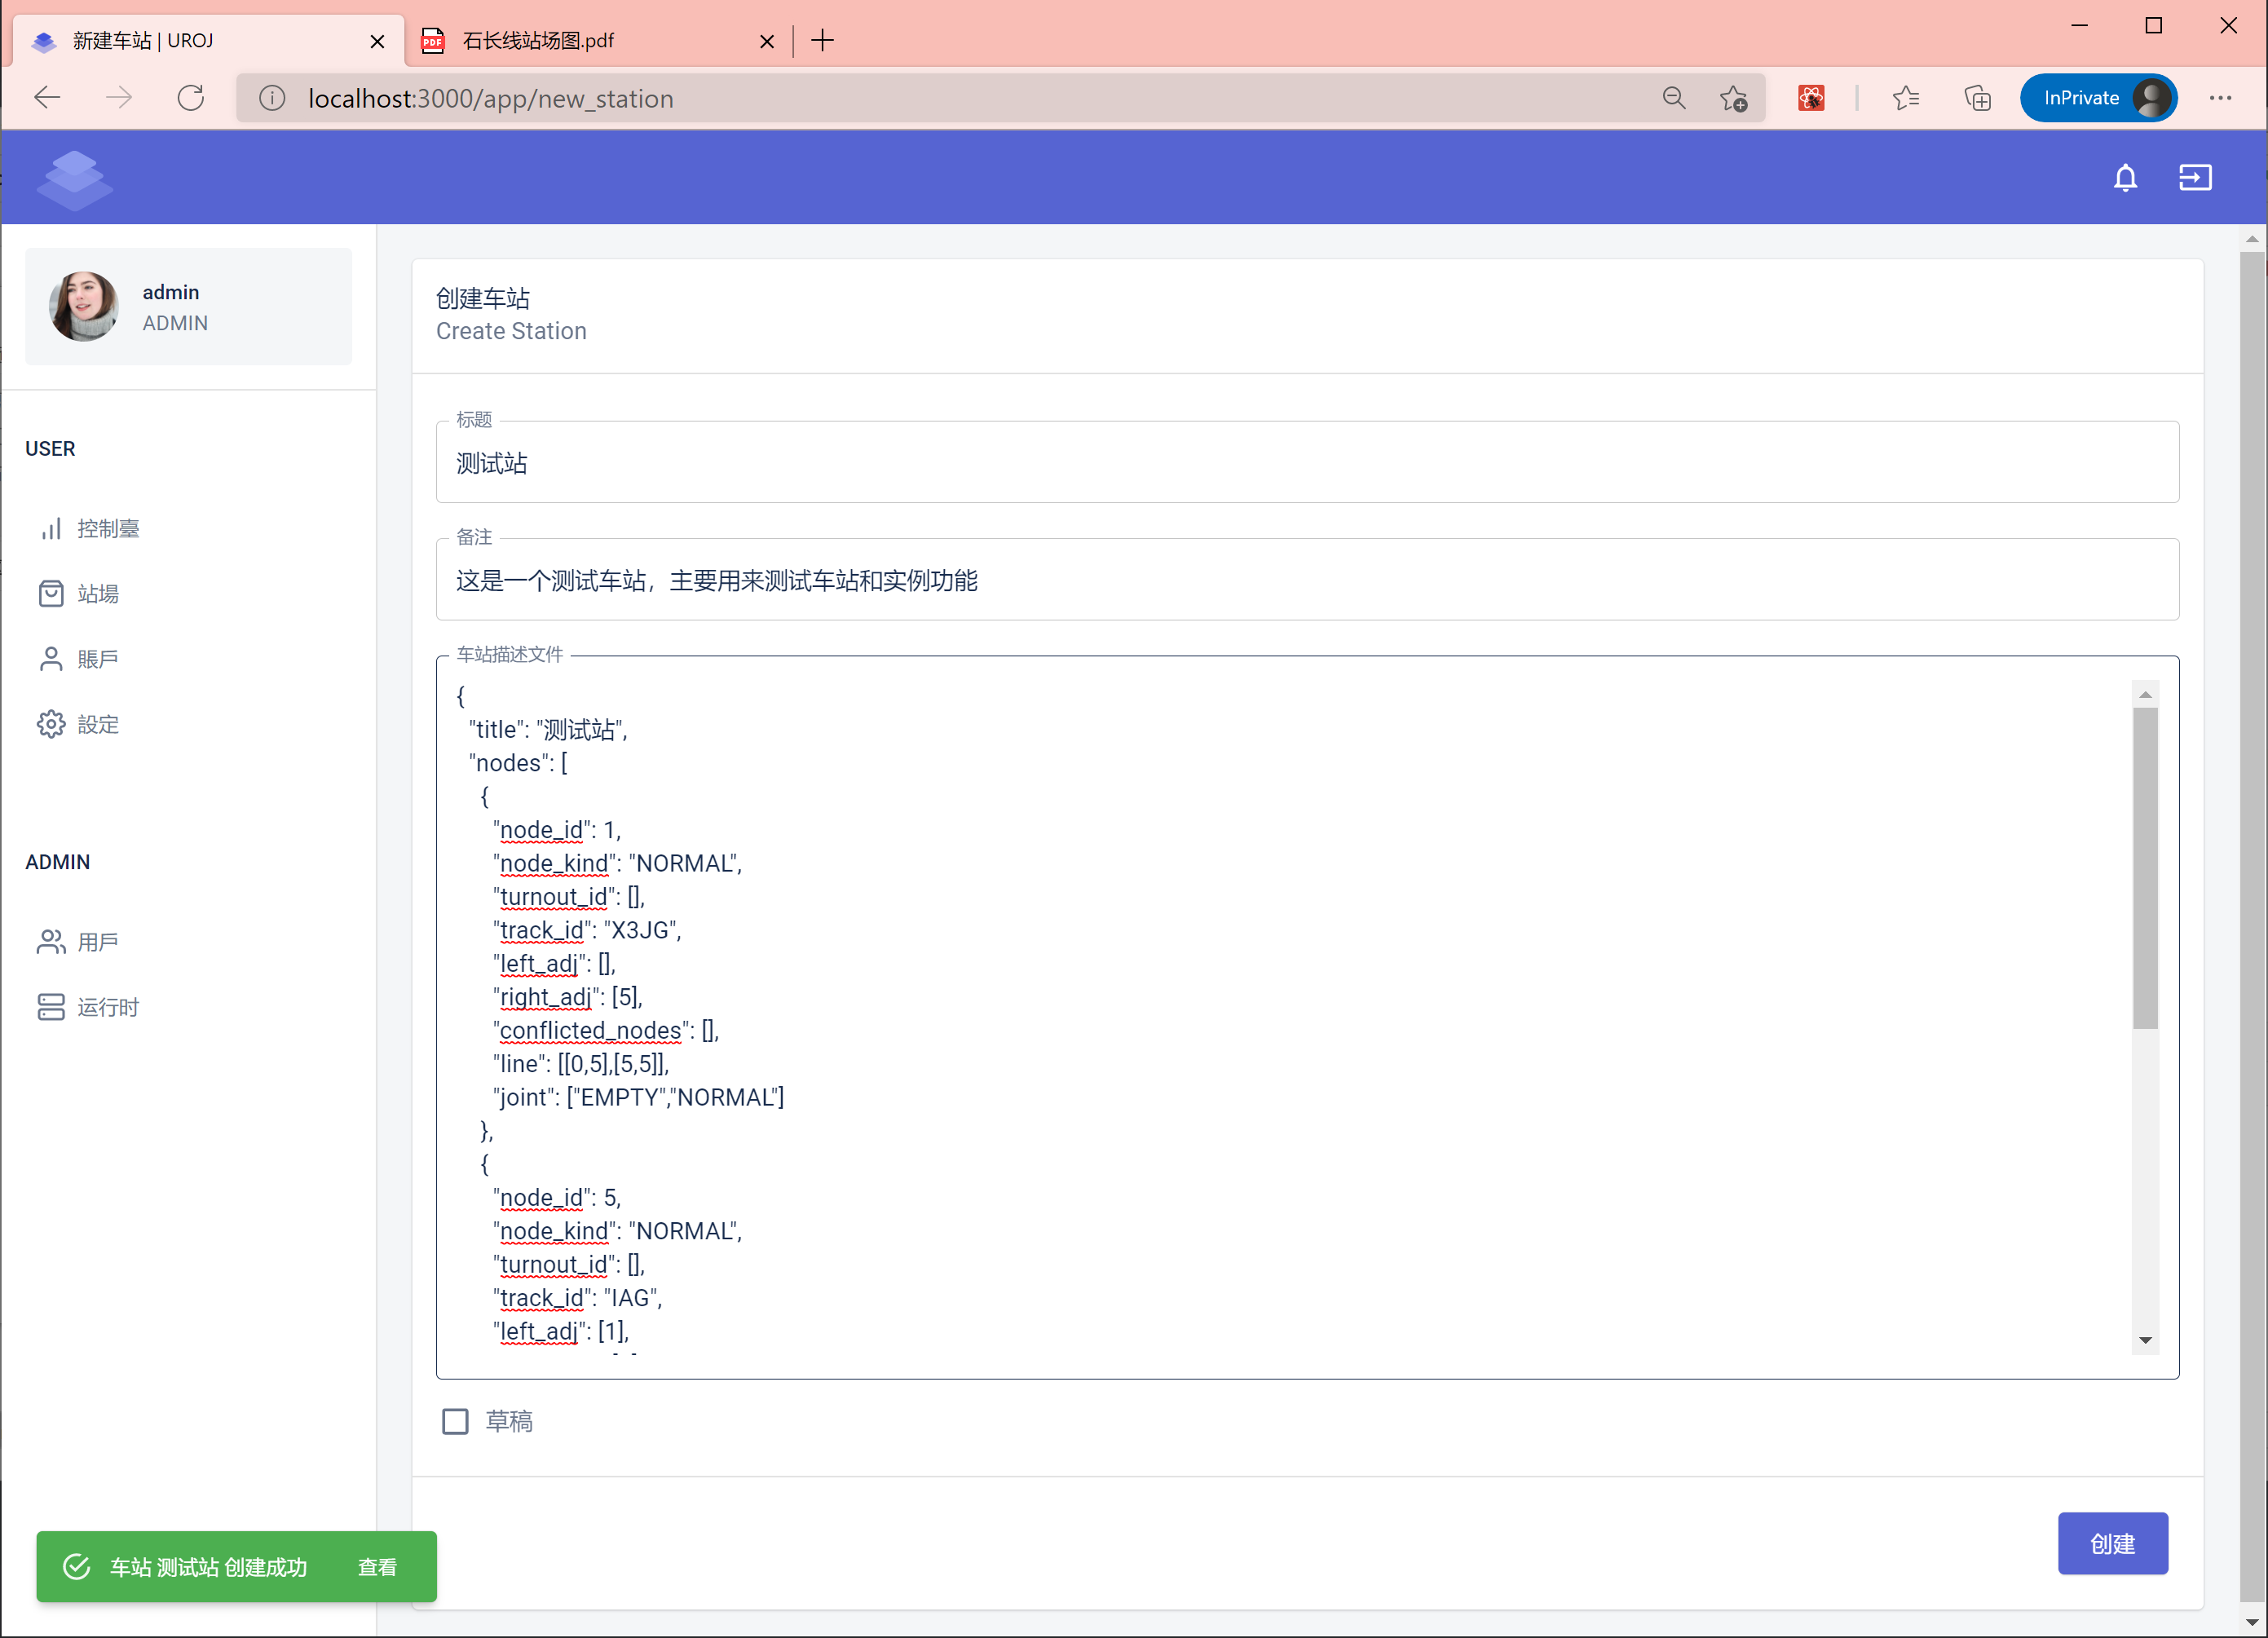
\includegraphics[width=\textwidth]{figures/png/create_sta_succ.png}
    \caption{\label{create_sta_succ}创建车站成功}
\end{figure}

\begin{figure}[htbp!]
    \centering
    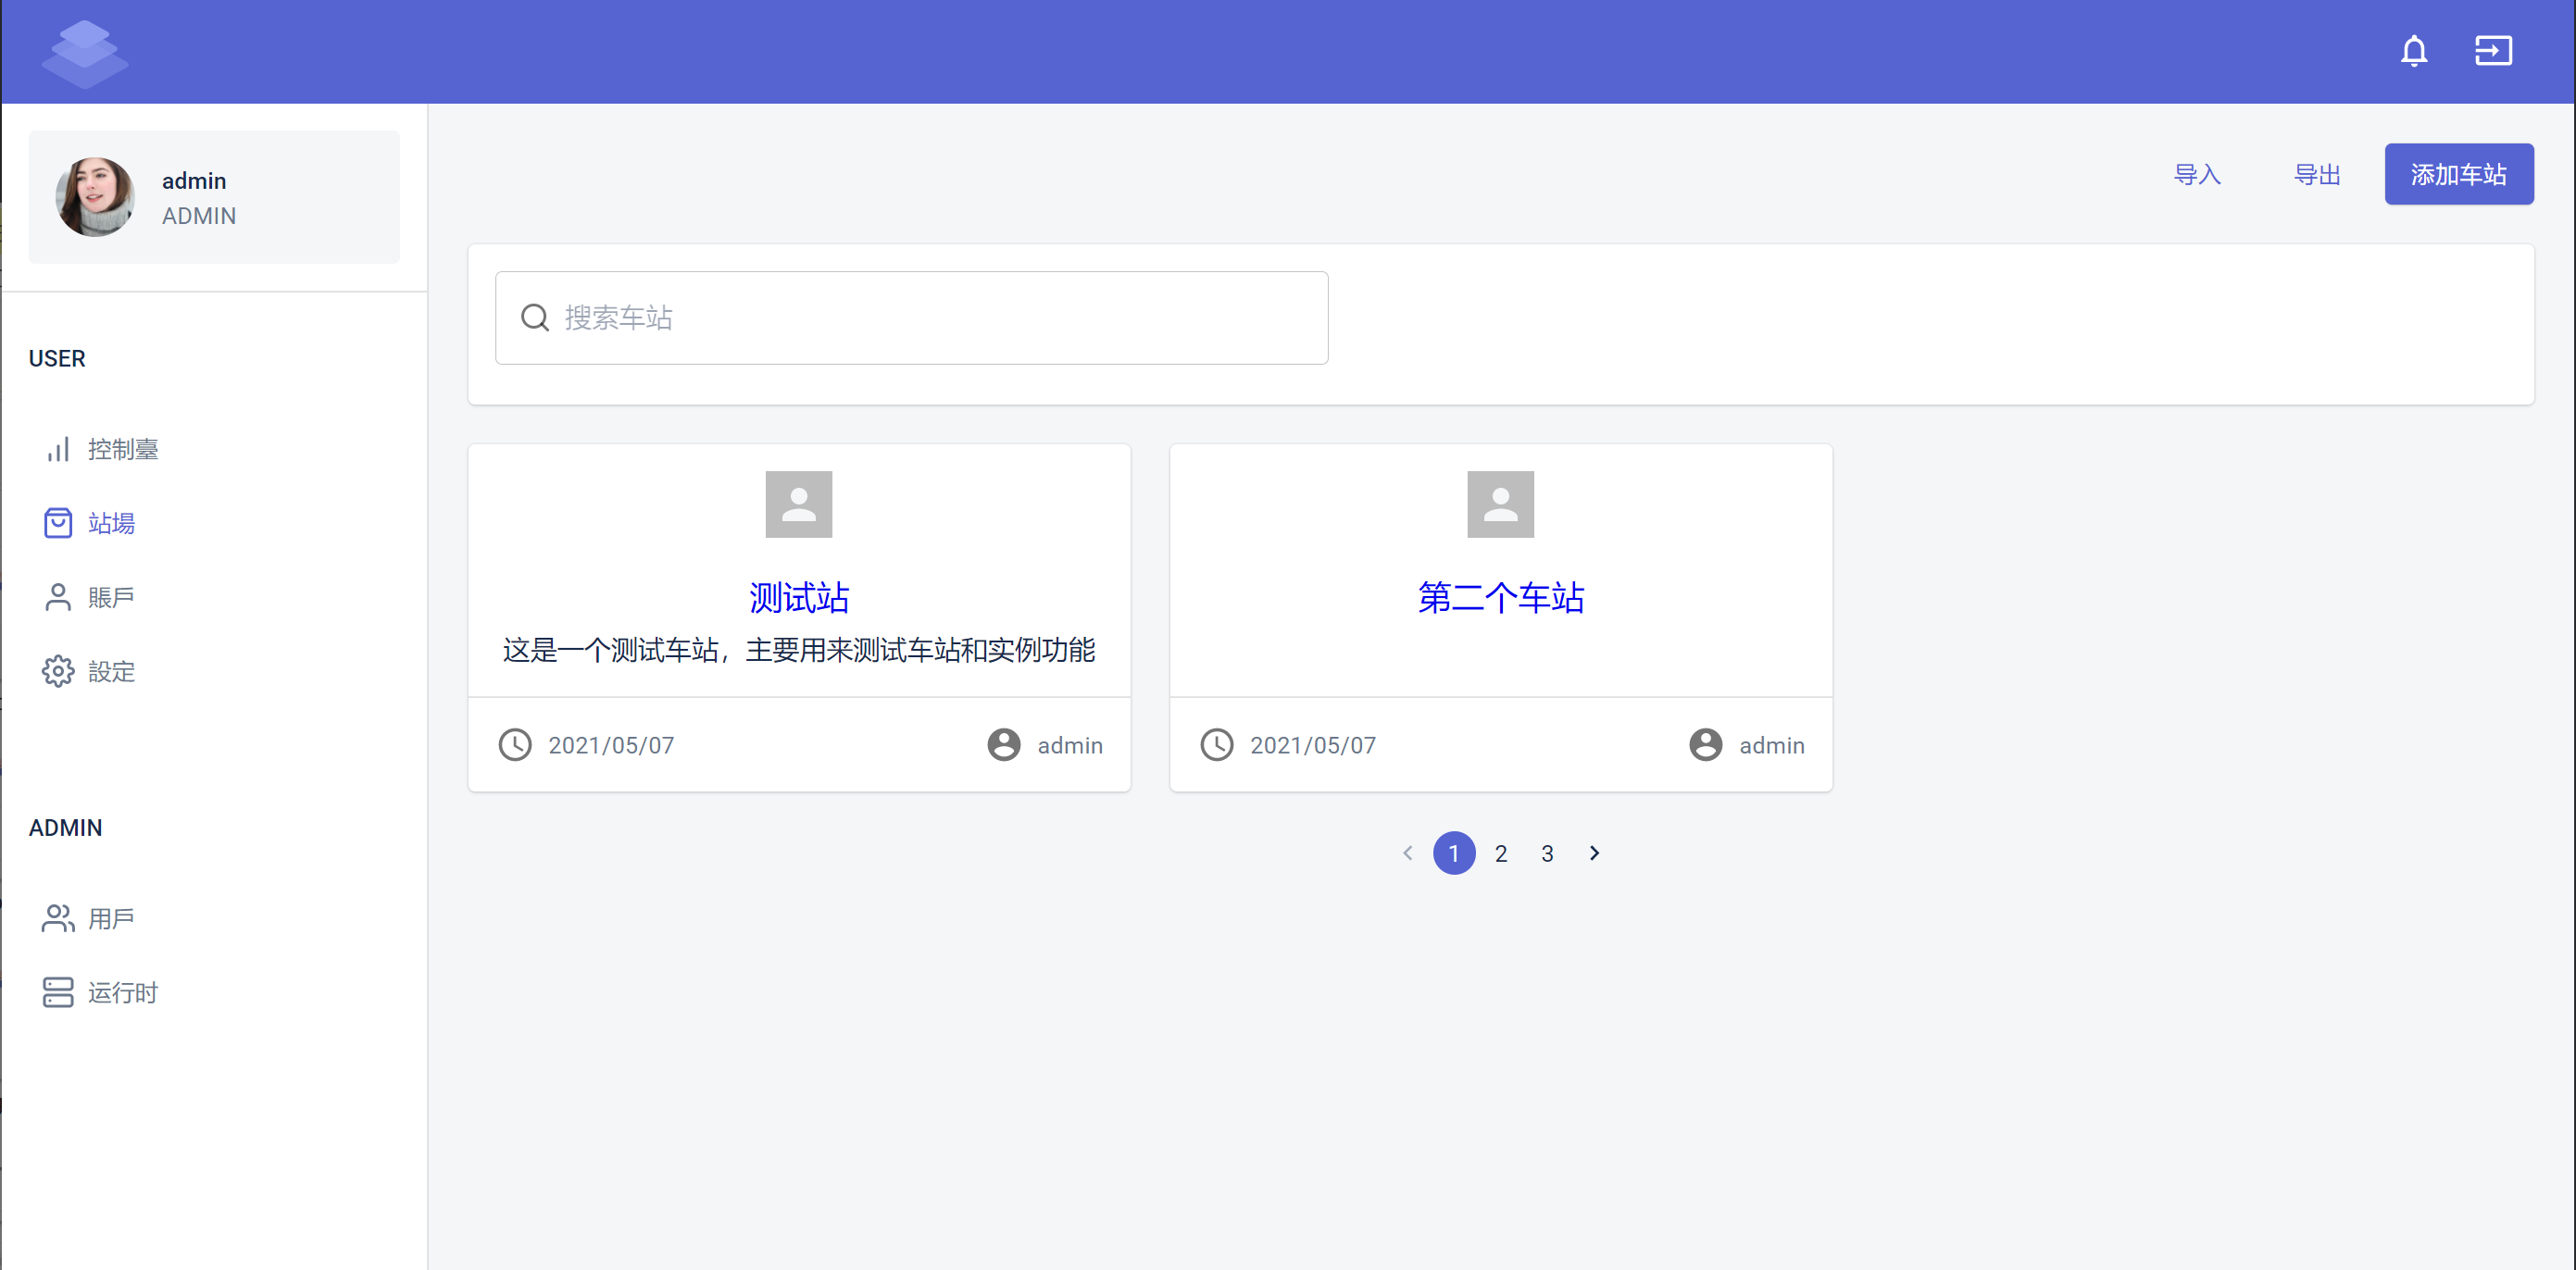
\includegraphics[width=\textwidth]{figures/png/station_list.png}
    \caption{\label{station_list}车站页面}
\end{figure}

\begin{figure}[htbp!]
    \centering
    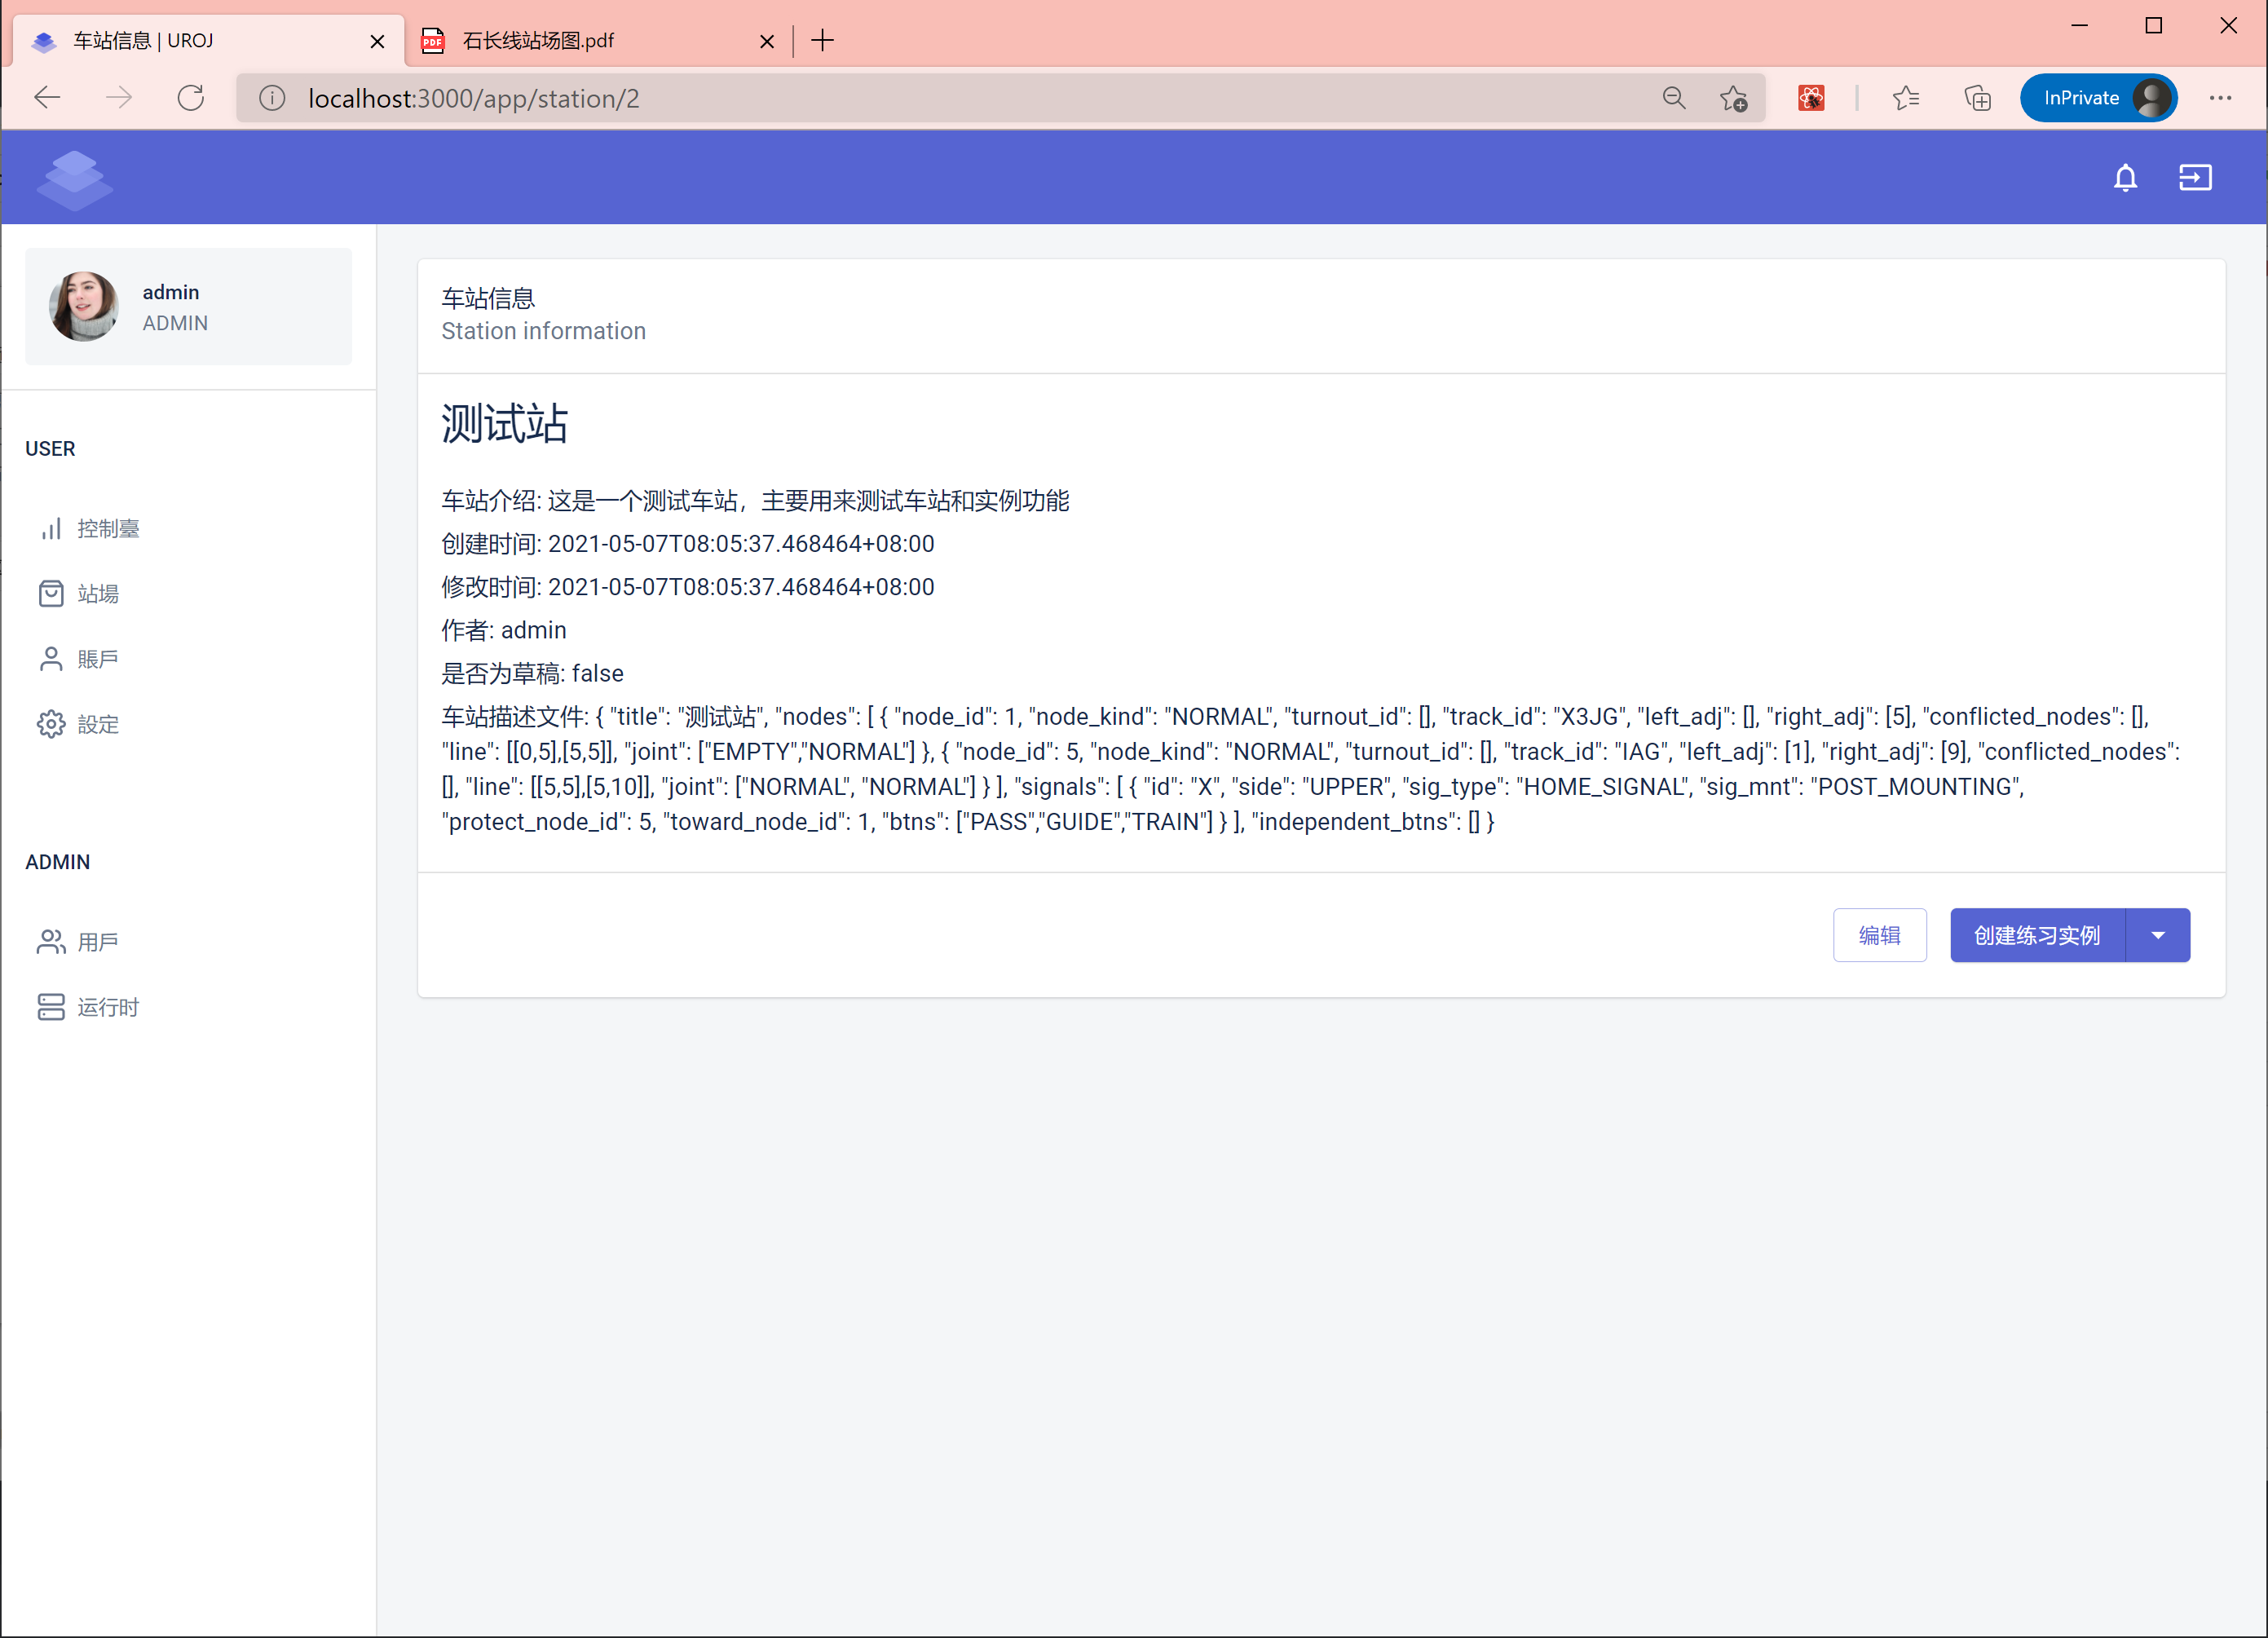
\includegraphics[width=\textwidth]{figures/png/station_info.png}
    \caption{\label{station_info}车站信息查看}
\end{figure}

\begin{figure}[htbp!]
    \centering
    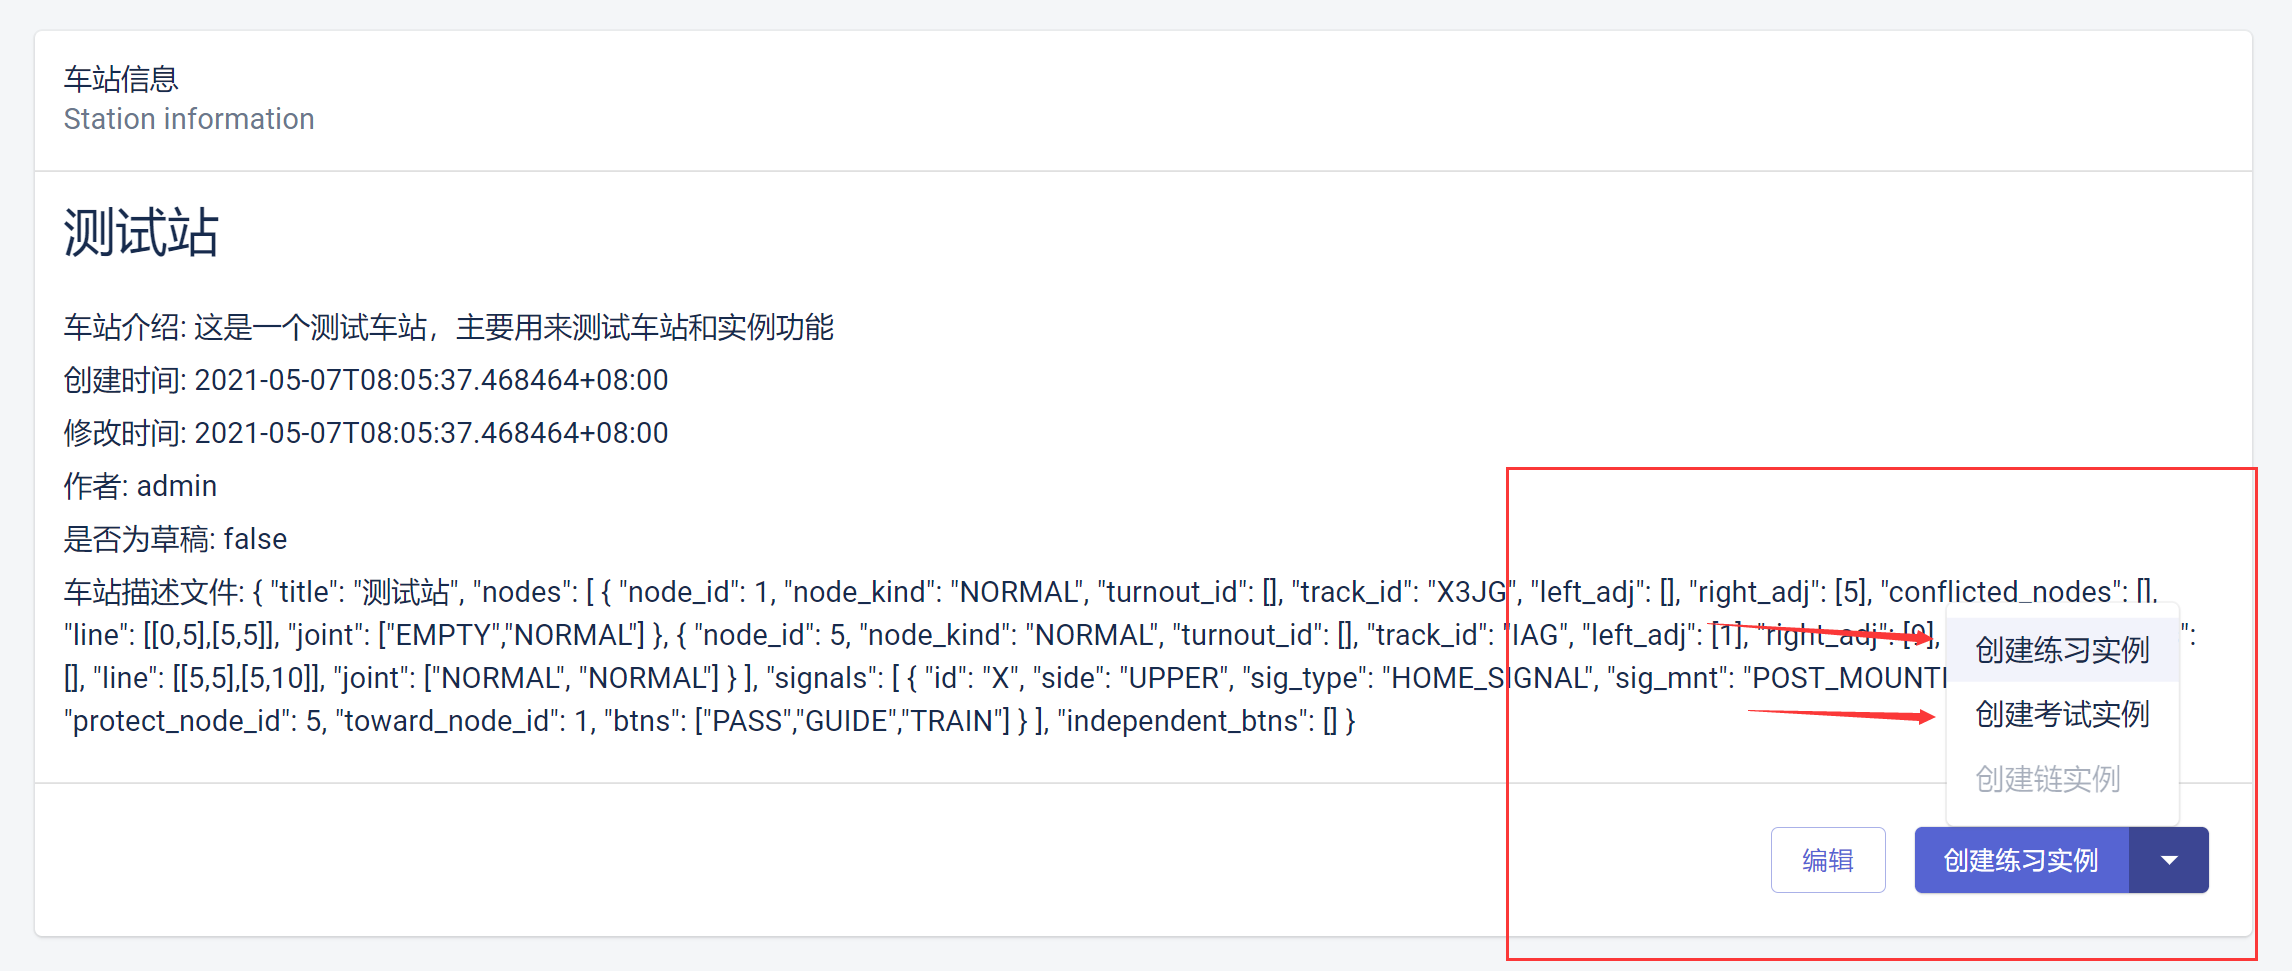
\includegraphics[width=\textwidth]{figures/png/create_btn.png}
    \caption{\label{create_btn}选择实例类型}
\end{figure}

\begin{figure}[htbp!]
    \centering
    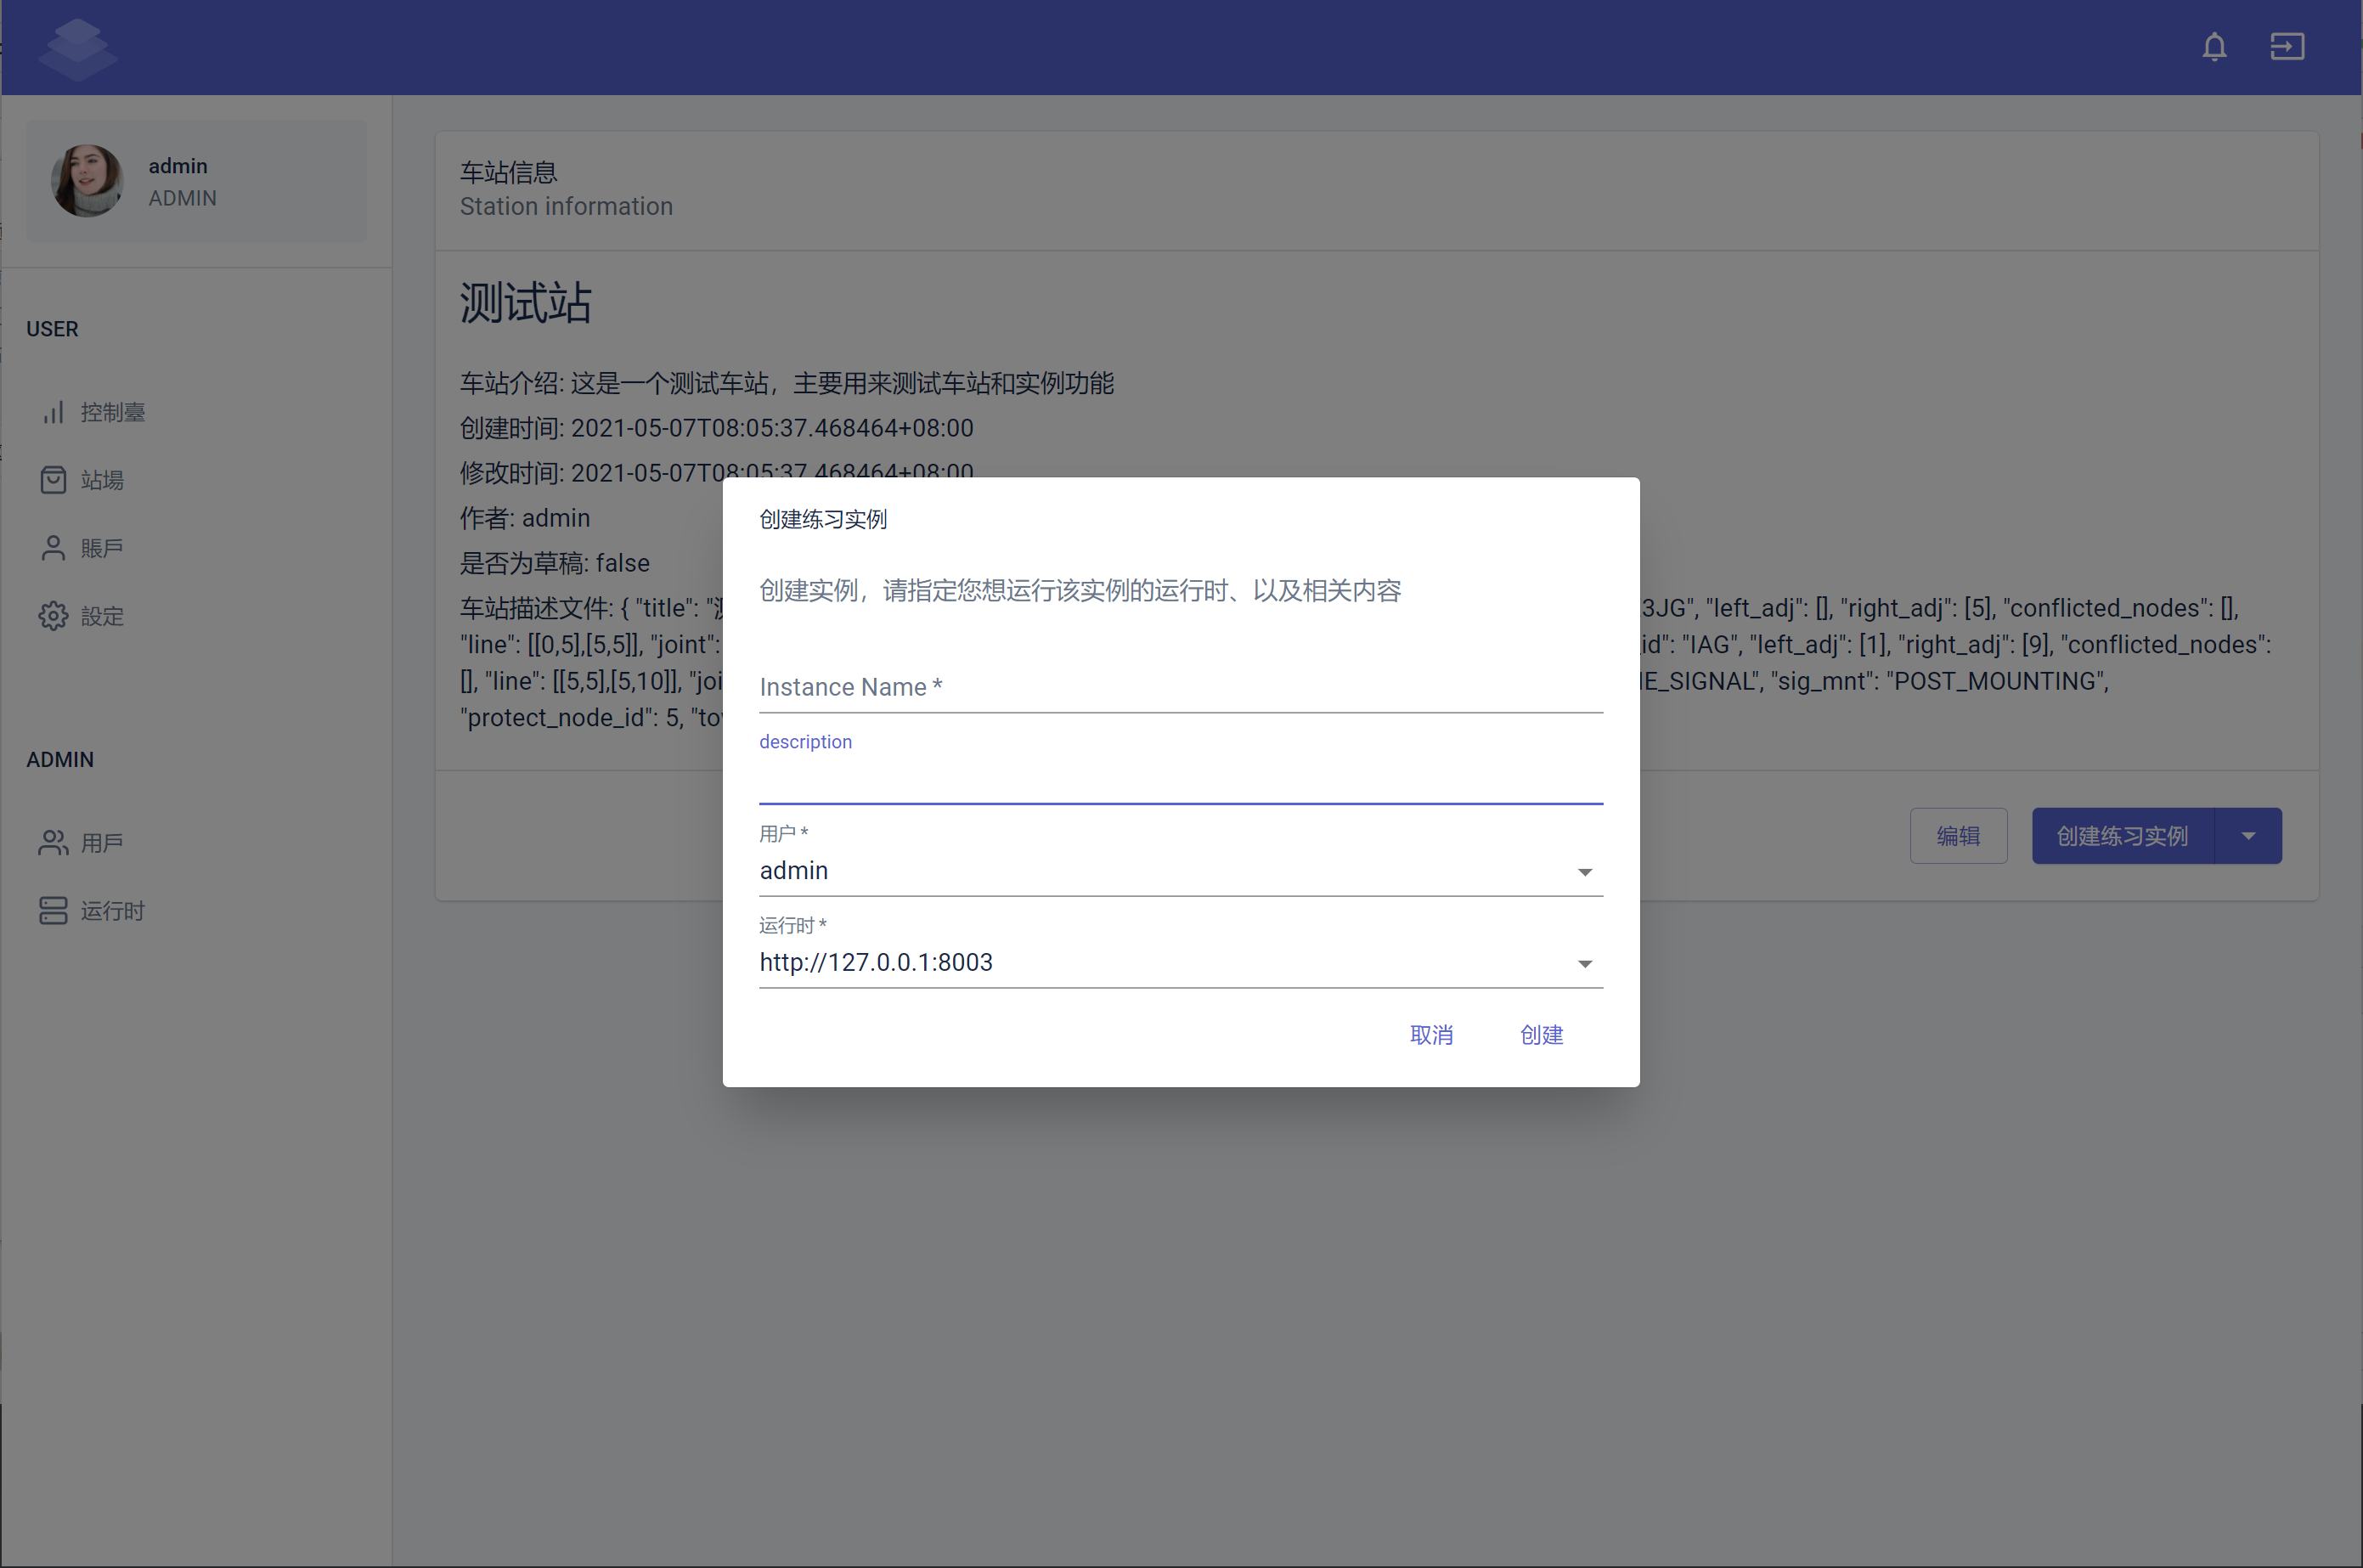
\includegraphics[width=\textwidth]{figures/png/dialog.png}
    \caption{\label{dialog}新建实例对话框}
\end{figure}

\begin{figure}[htbp!]
    \centering
    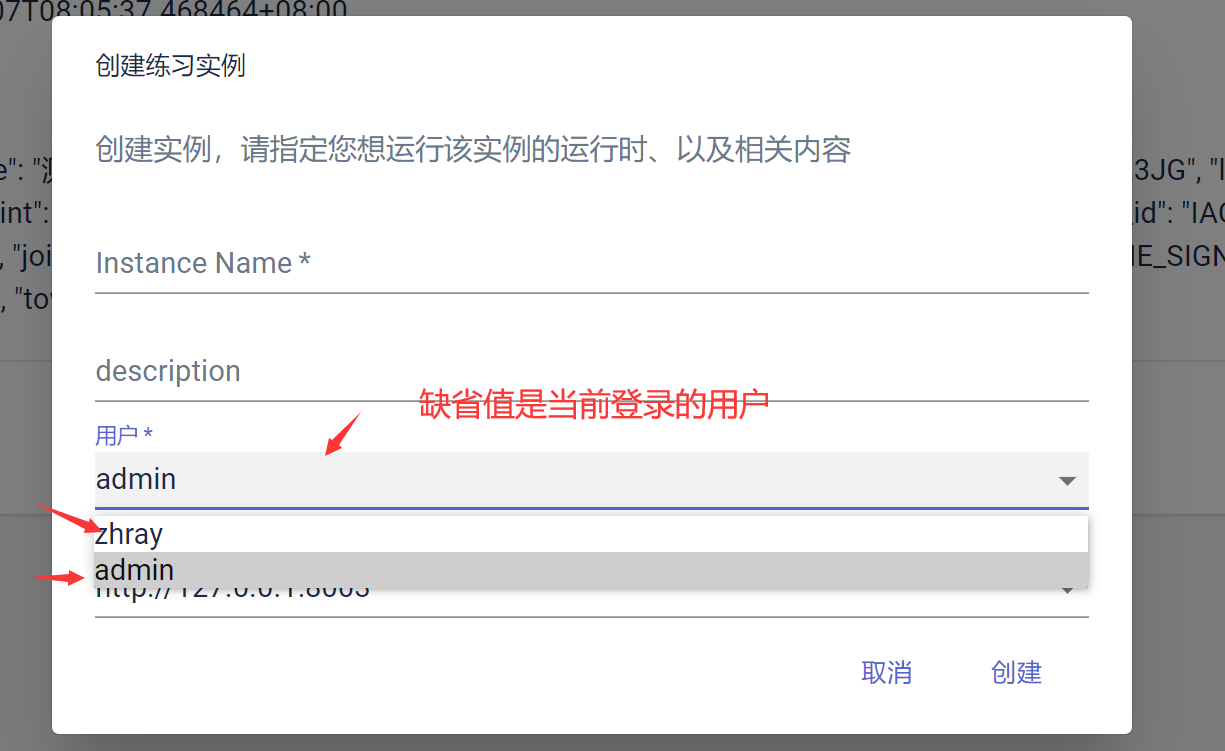
\includegraphics[width=\textwidth]{figures/png/dialog_detail.png}
    \caption{\label{dialog_detail}用户选单缺省}
\end{figure}

\begin{figure}[htbp!]
    \centering
    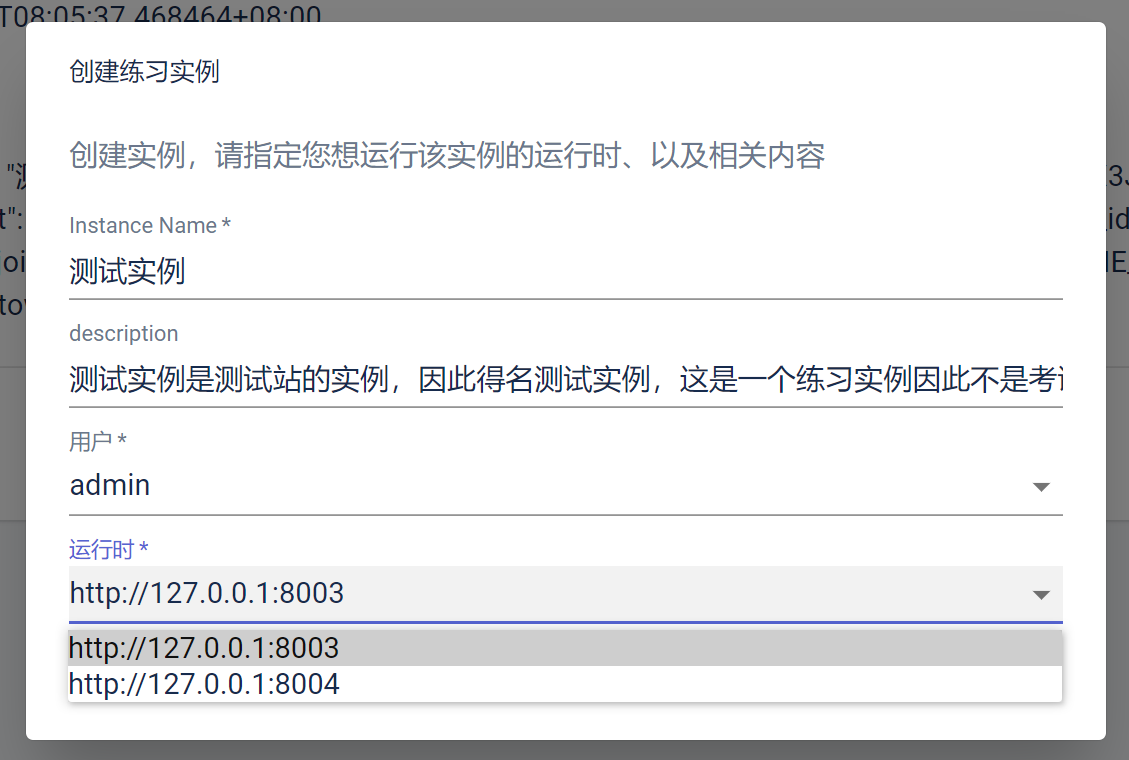
\includegraphics[width=\textwidth]{figures/png/runtime_list.png}
    \caption{\label{runtime_list}运行时选单}
\end{figure}

\begin{figure}[htbp!]
    \centering
    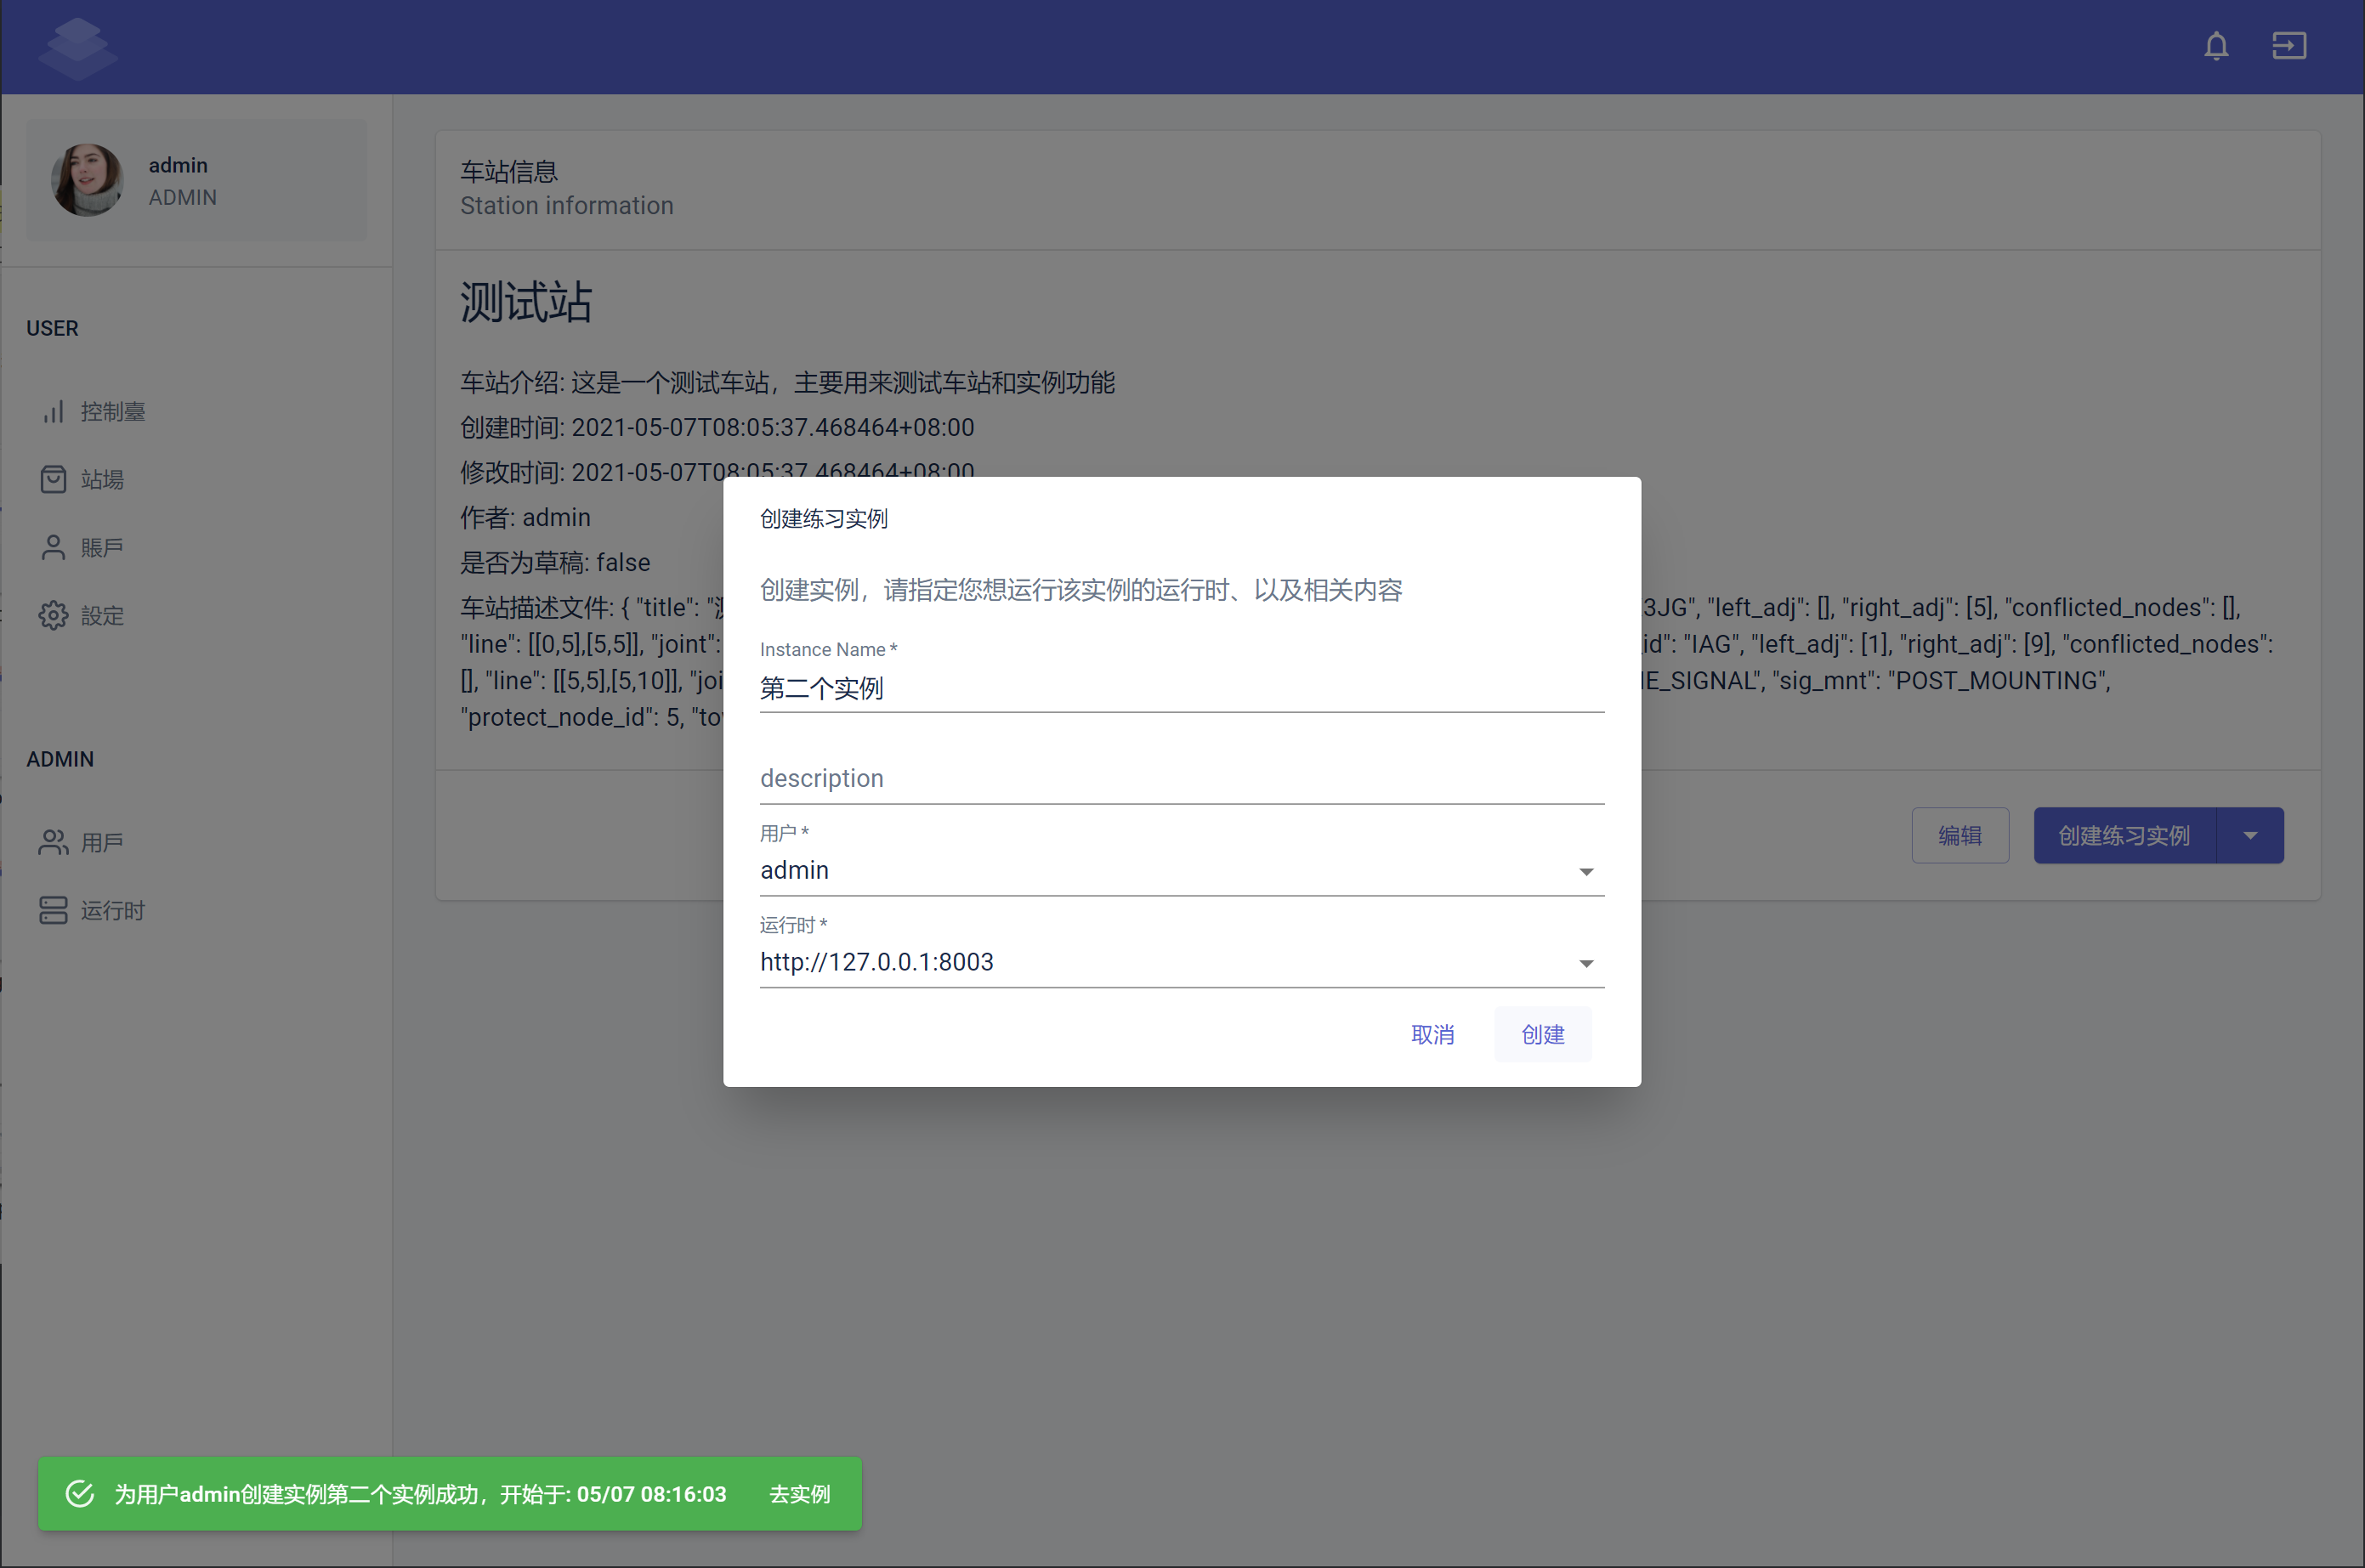
\includegraphics[width=\textwidth]{figures/png/dialog_succ.png}
    \caption{\label{dialog_succ}创建实例成功}
\end{figure}

\begin{figure}[htbp!]
    \centering
    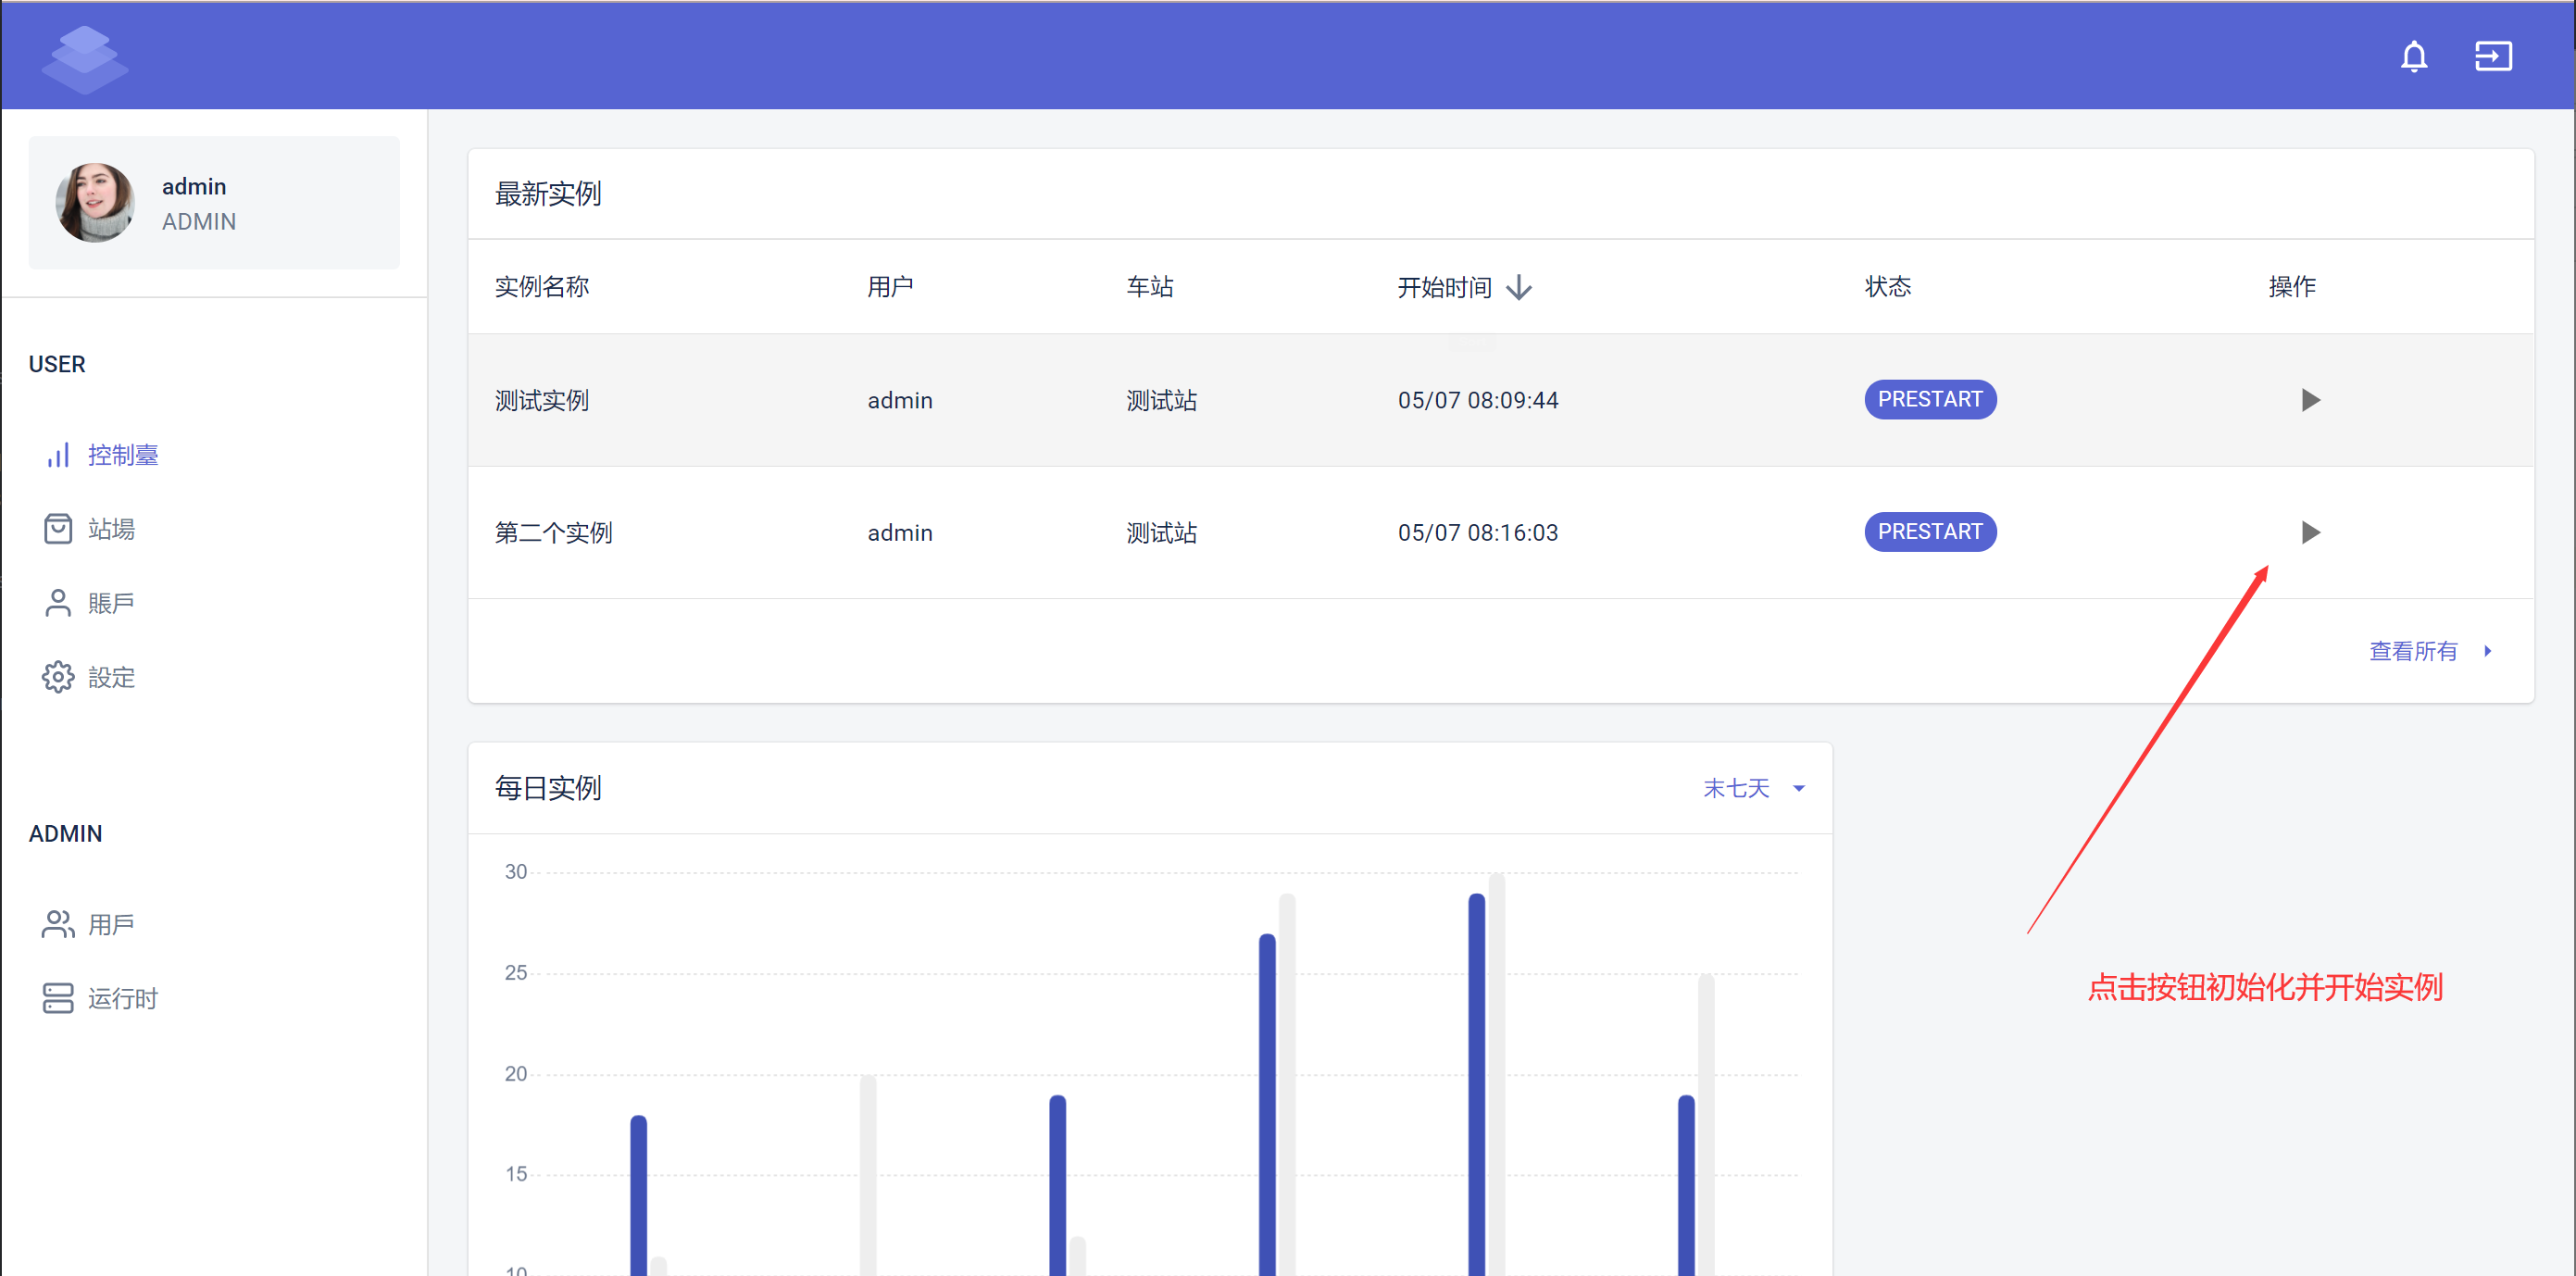
\includegraphics[width=\textwidth]{figures/png/after_create.png}
    \caption{\label{after_create}创建实例后运行实例前}
\end{figure}

\begin{figure}[htbp!]
    \centering
    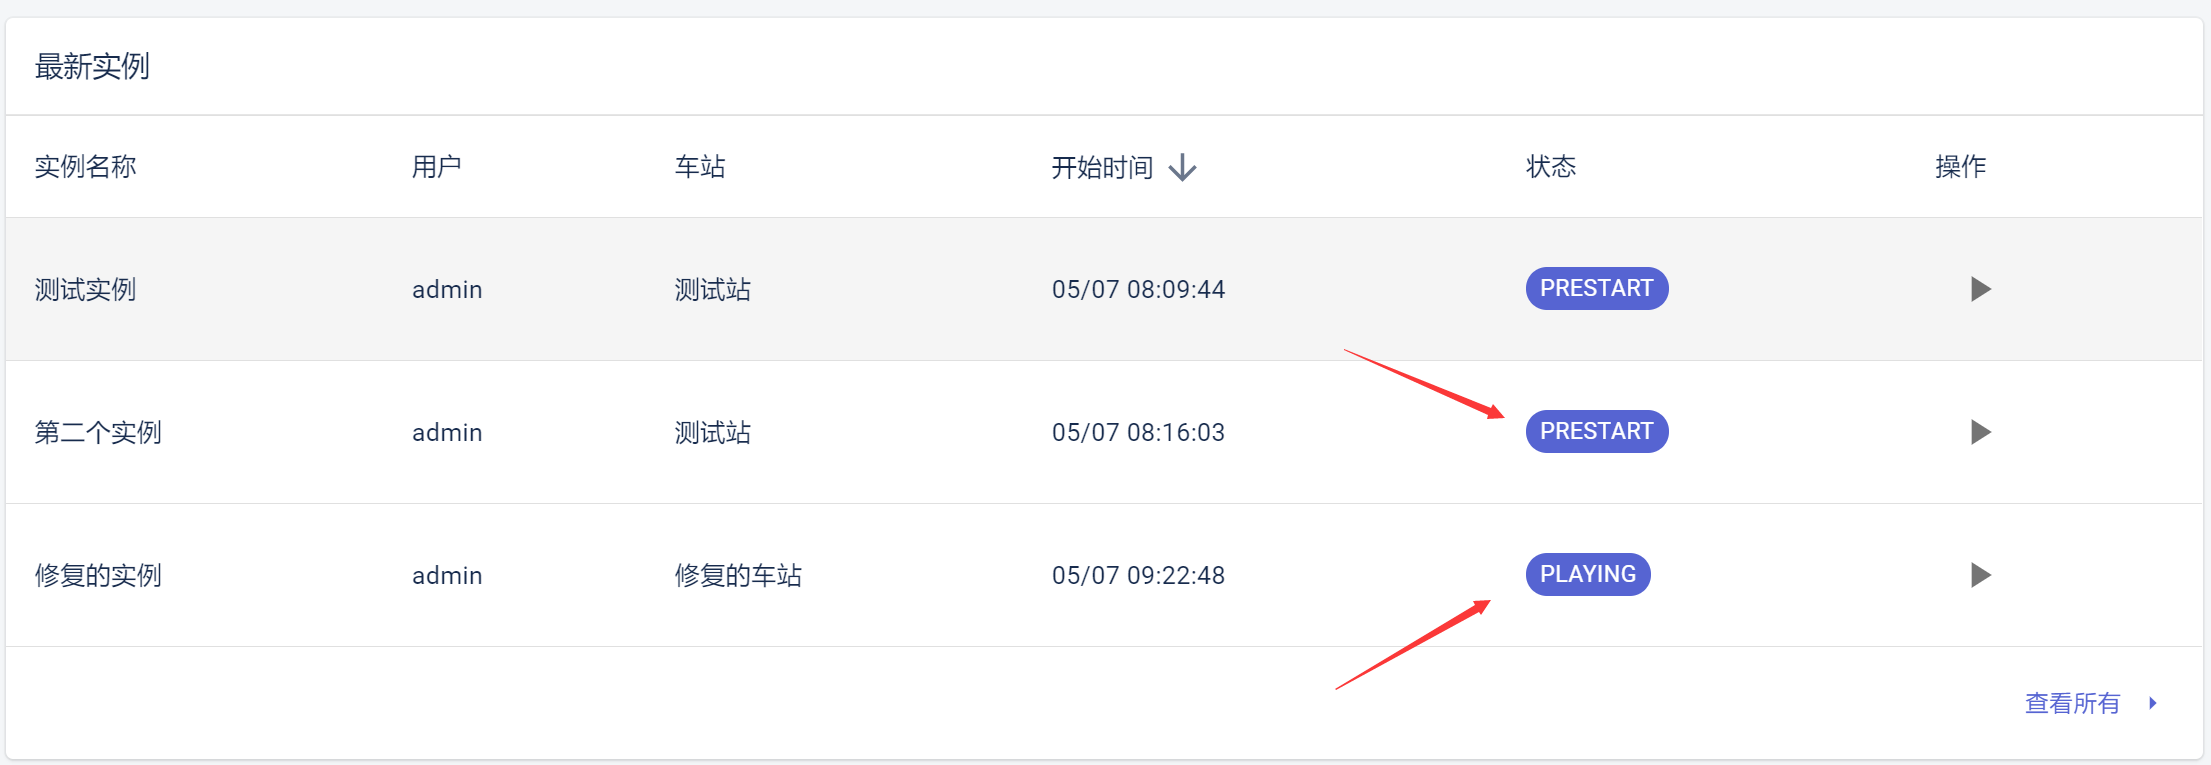
\includegraphics[width=\textwidth]{figures/png/3rd.png}
    \caption{\label{3rd}运行实例后}
\end{figure}

在图 \ref{after_create} 中,若当前时间未满开始时间,则开始的三角按钮不能被
按下,也就是前文所述的双重保证。在按下开始按钮后,实例在运行时中被
初始化、运行、实例状态从 PRESTART 变为 PLAYING。表现层的网页
则跳转至实例界面。

\subsection{实例界面}